\pagestyle{n-1}
\label{n-1}

\pagebreak


\begin{center}
\hspace*{.5cm}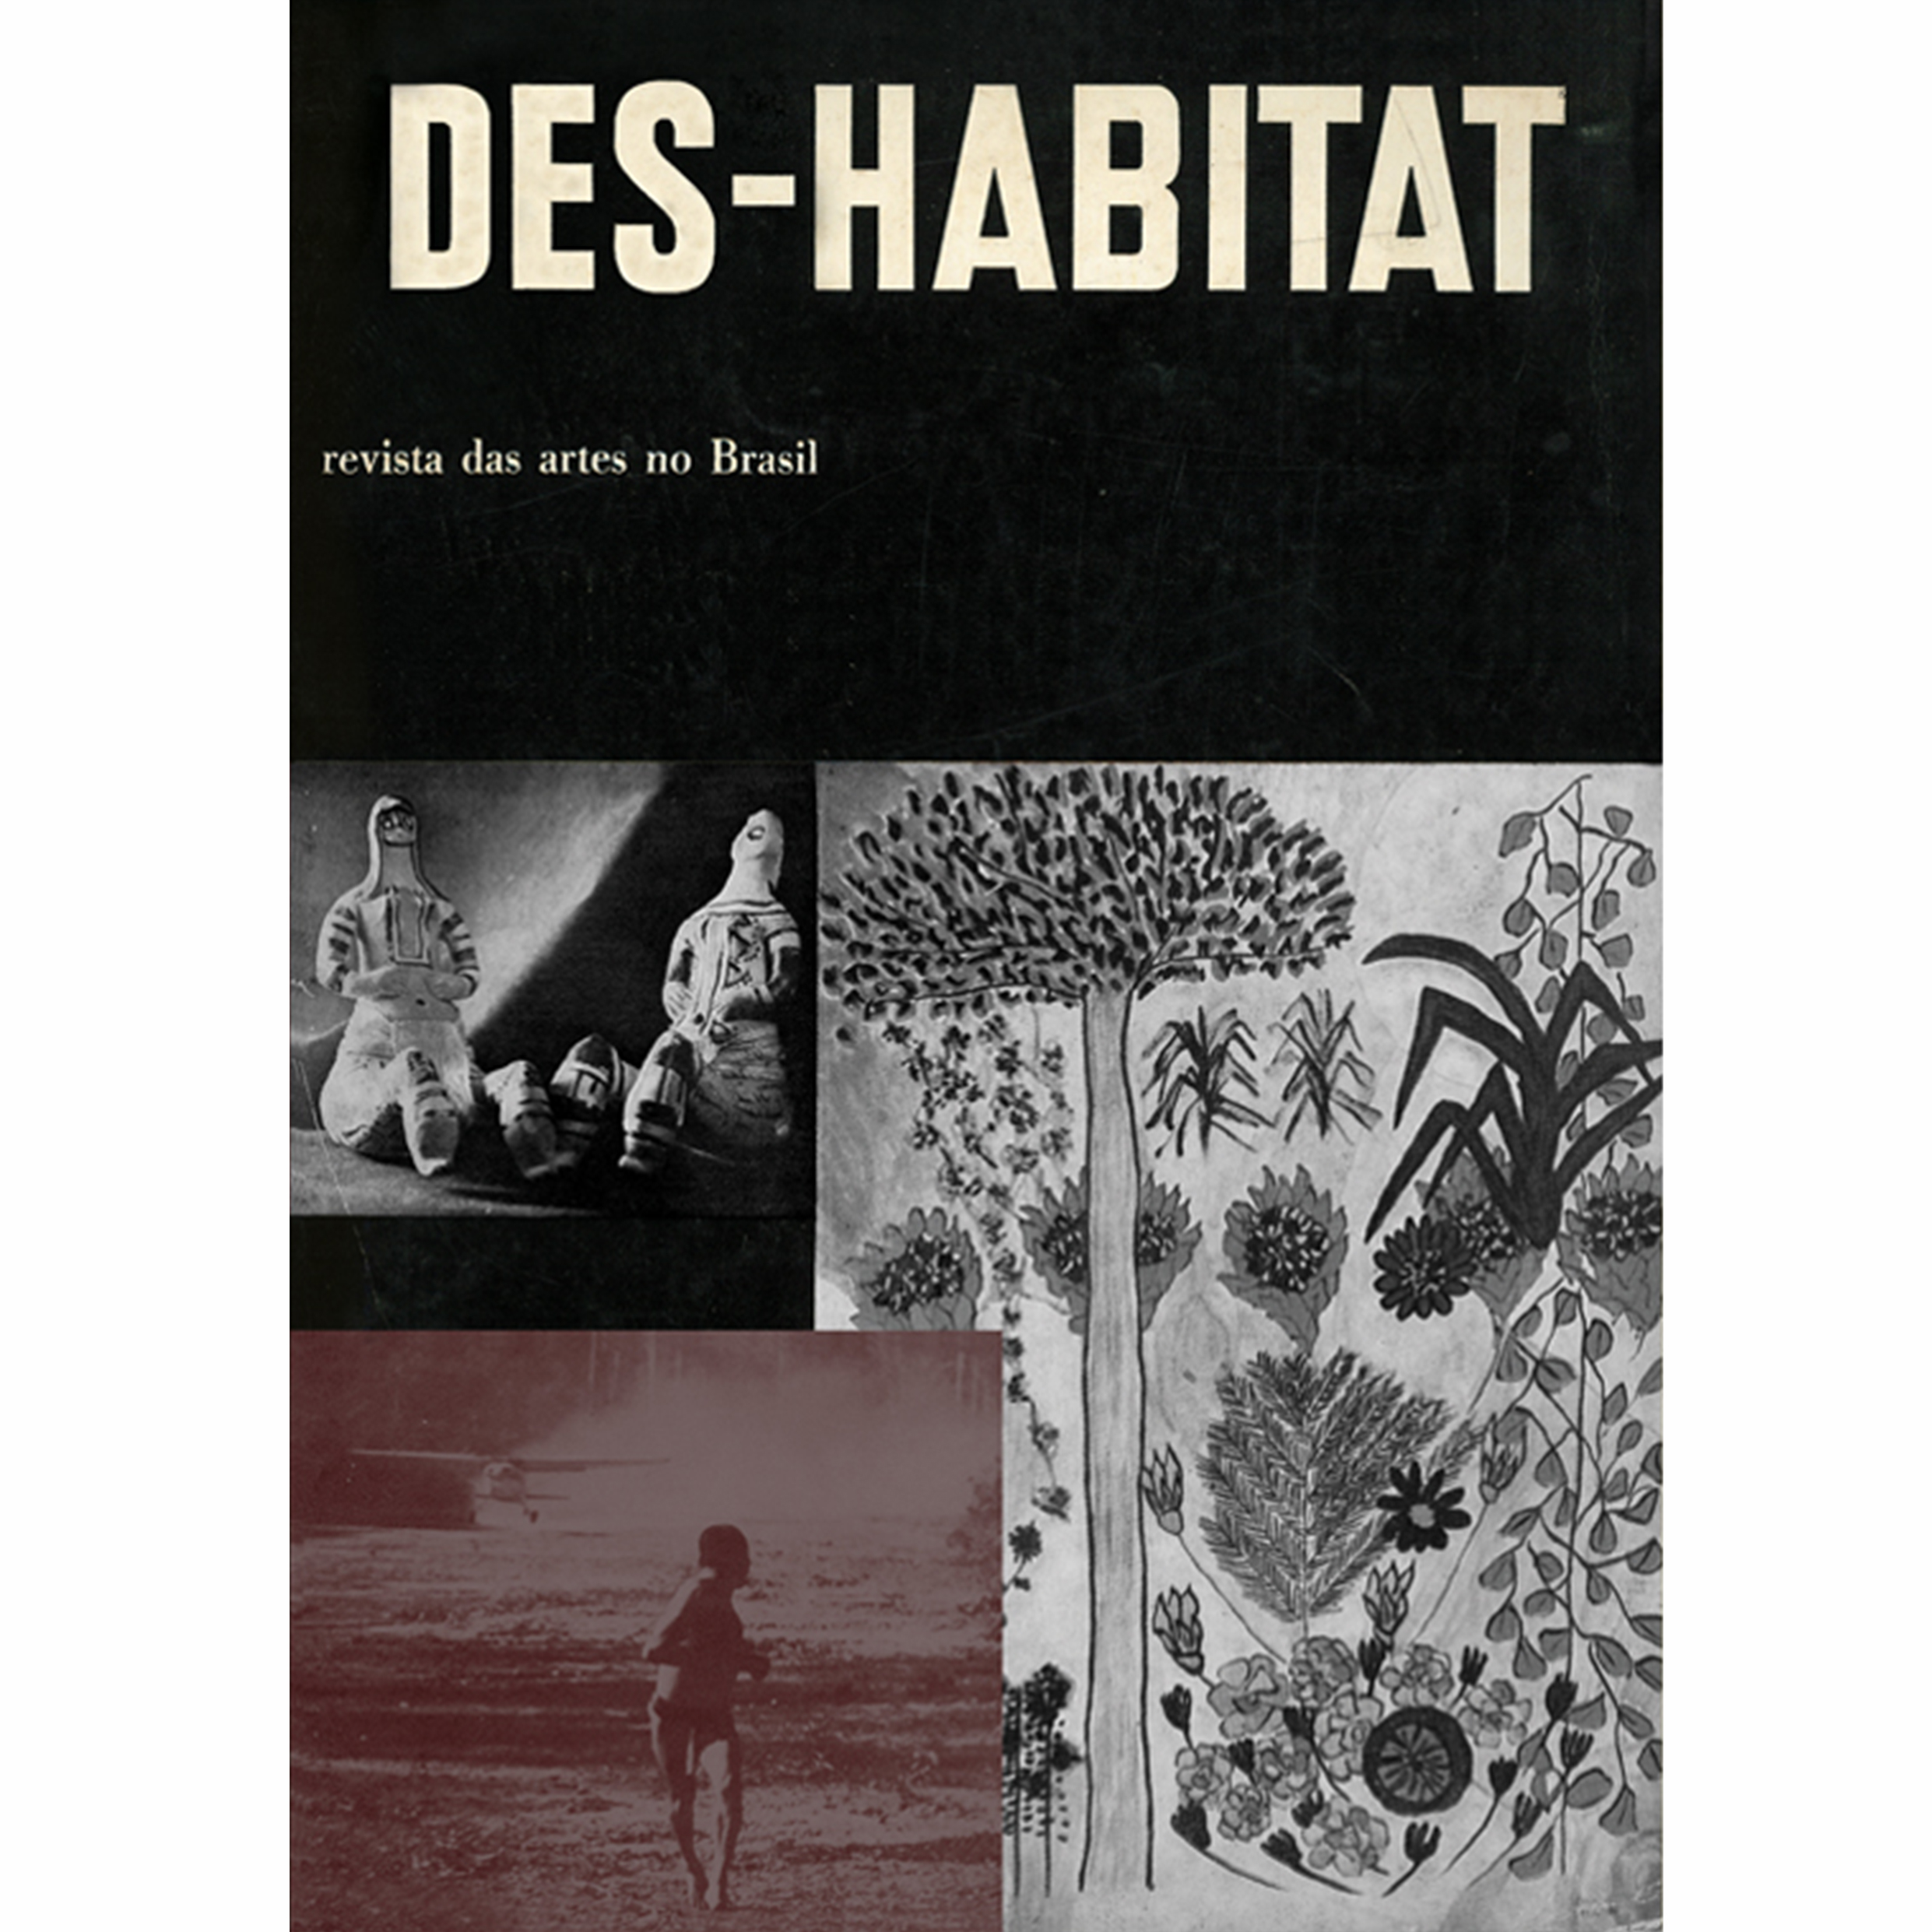
\includegraphics[width=74mm]{./CAPAS/N-1_HABITAT.jpg}
\end{center}

\hspace*{-7cm}\hrulefill\hspace*{-7cm}

\medskip

\noindent{}Neste ensaio visual, Paulo Tavares intervém em \textit{Habitat}, revista de artes e design editada pela arquiteta Lina Bo Bardi nos anos 1950. \hlc{Resignificando imagens e imaginários dominantes, \textit{Des-Habitat} nos carrega através de uma narrativa visual sobre a colonialidade da arquitetura moderna e suas mídias}, abrindo um horizonte para a potencial descolonização de seus legados. Com ensaio e design de Paulo Tavares, e prefácio da curadora Marion von Osten, em uma parceria entre agência autônoma e n-1 edições.

\vfill

\hspace*{-.4cm}\begin{minipage}[c]{1\linewidth}
\small\textbf{
\hspace*{-.1cm}Editora: n-1\\
Título: Des-Habitat\\
Autor: Paulo Tavares\\ 
ISBN: 978-65-86941-39-5\\
Páginas: 97\\
Formato: 23,5x33\,cm\\
Preço: R\$ 70,00\\
}
\end{minipage}

\pagebreak %PRAGMATISMO PULSIONAL


\begin{center}
\hspace*{-3.6cm}\raisebox{5cm}{\rotatebox[origin=t]{90}{\huge\textbf{Lançamento}}}
\hspace*{3.1cm}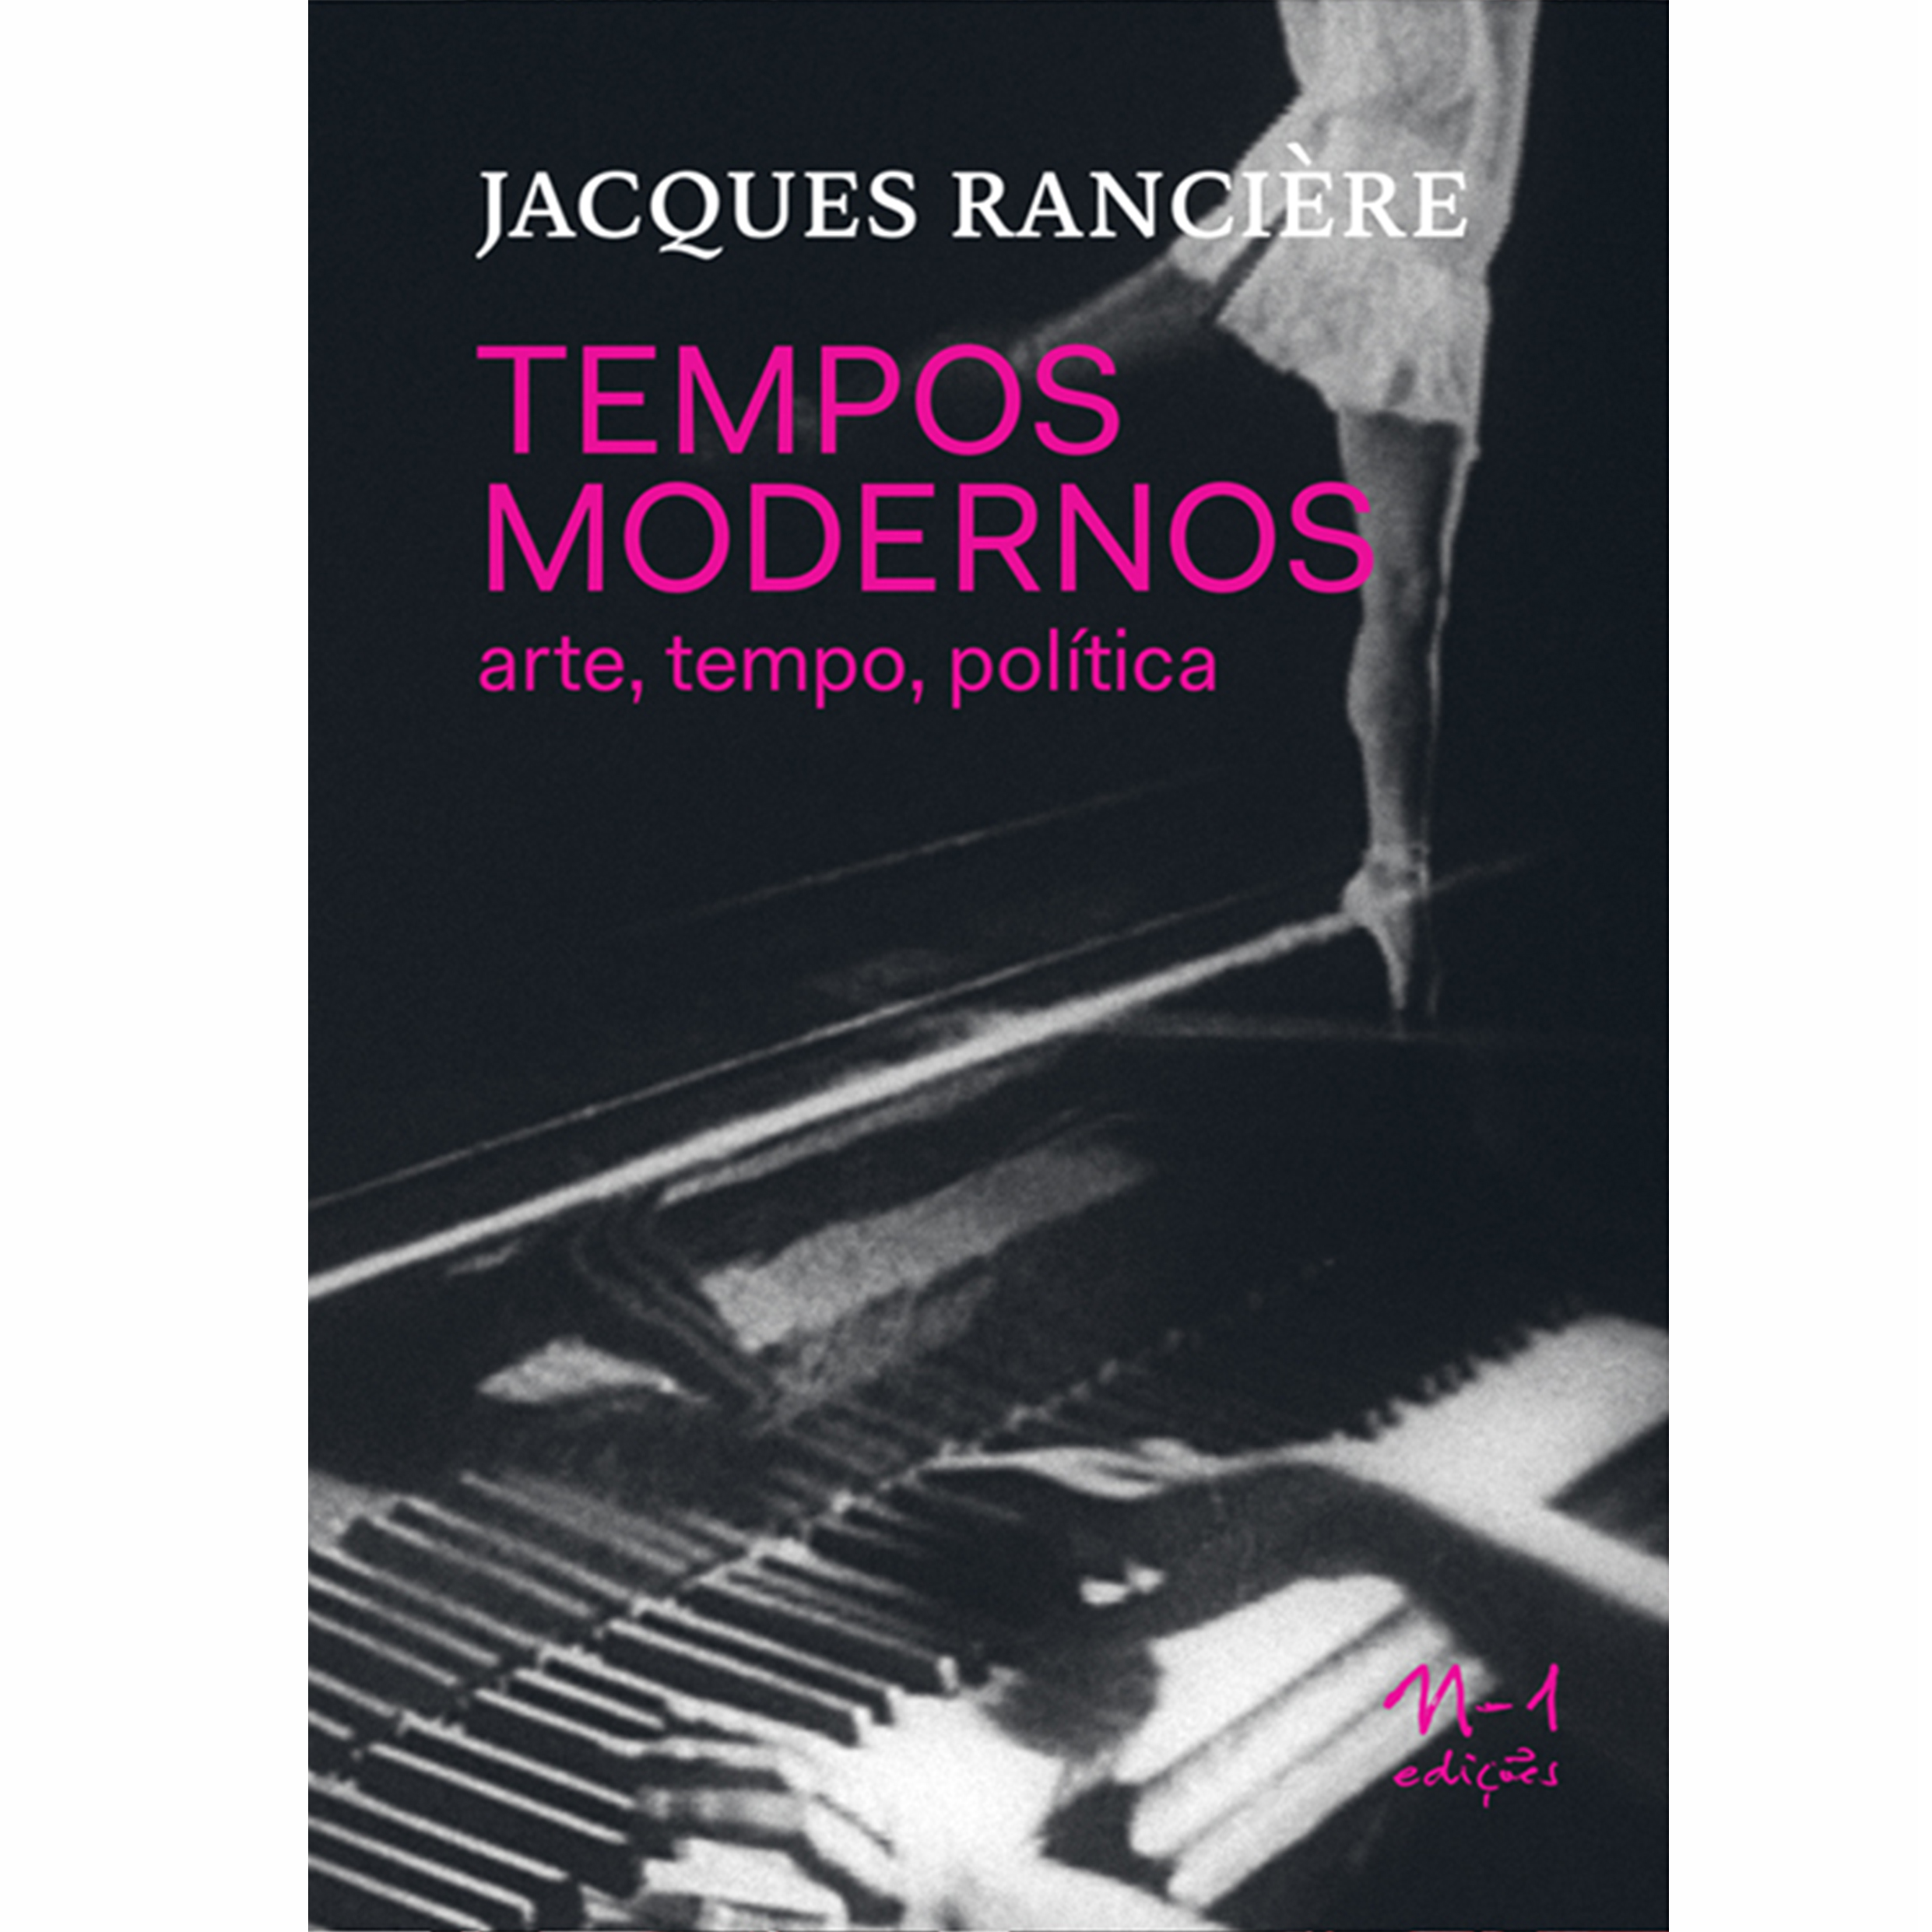
\includegraphics[width=74mm]{./CAPAS/N-1_JACQUES.jpg}
\end{center}

\hspace*{-7cm}\hrulefill\hspace*{-7cm}

\medskip

\noindent{}Não há tempo moderno, mas tempos modernos, \hlc{maneiras diferentes ou contraditórias de agenciar as temporalidades das artes do movimento}, suas continuidades, seus cortes, seus reajustes e suas retomadas, para produzir obras que respondam às condições do presente e às exigências do futuro.
\vfill

\hspace*{-.4cm}\begin{minipage}[c]{.8\linewidth}
\small\textbf{
\hspace*{-.1cm}Editora: n-1\\
Título: Tempos modernos: arte, tempo, política\\
Autor: Jacques Rancière\\ 
ISBN: 978-65-86941-40-1\\
Páginas: 160\\
Formato: 17x12\,cm\\
Preço: R\$ 65,00\\
}
\end{minipage}

\pagebreak

\begin{center}
\hspace*{.5cm}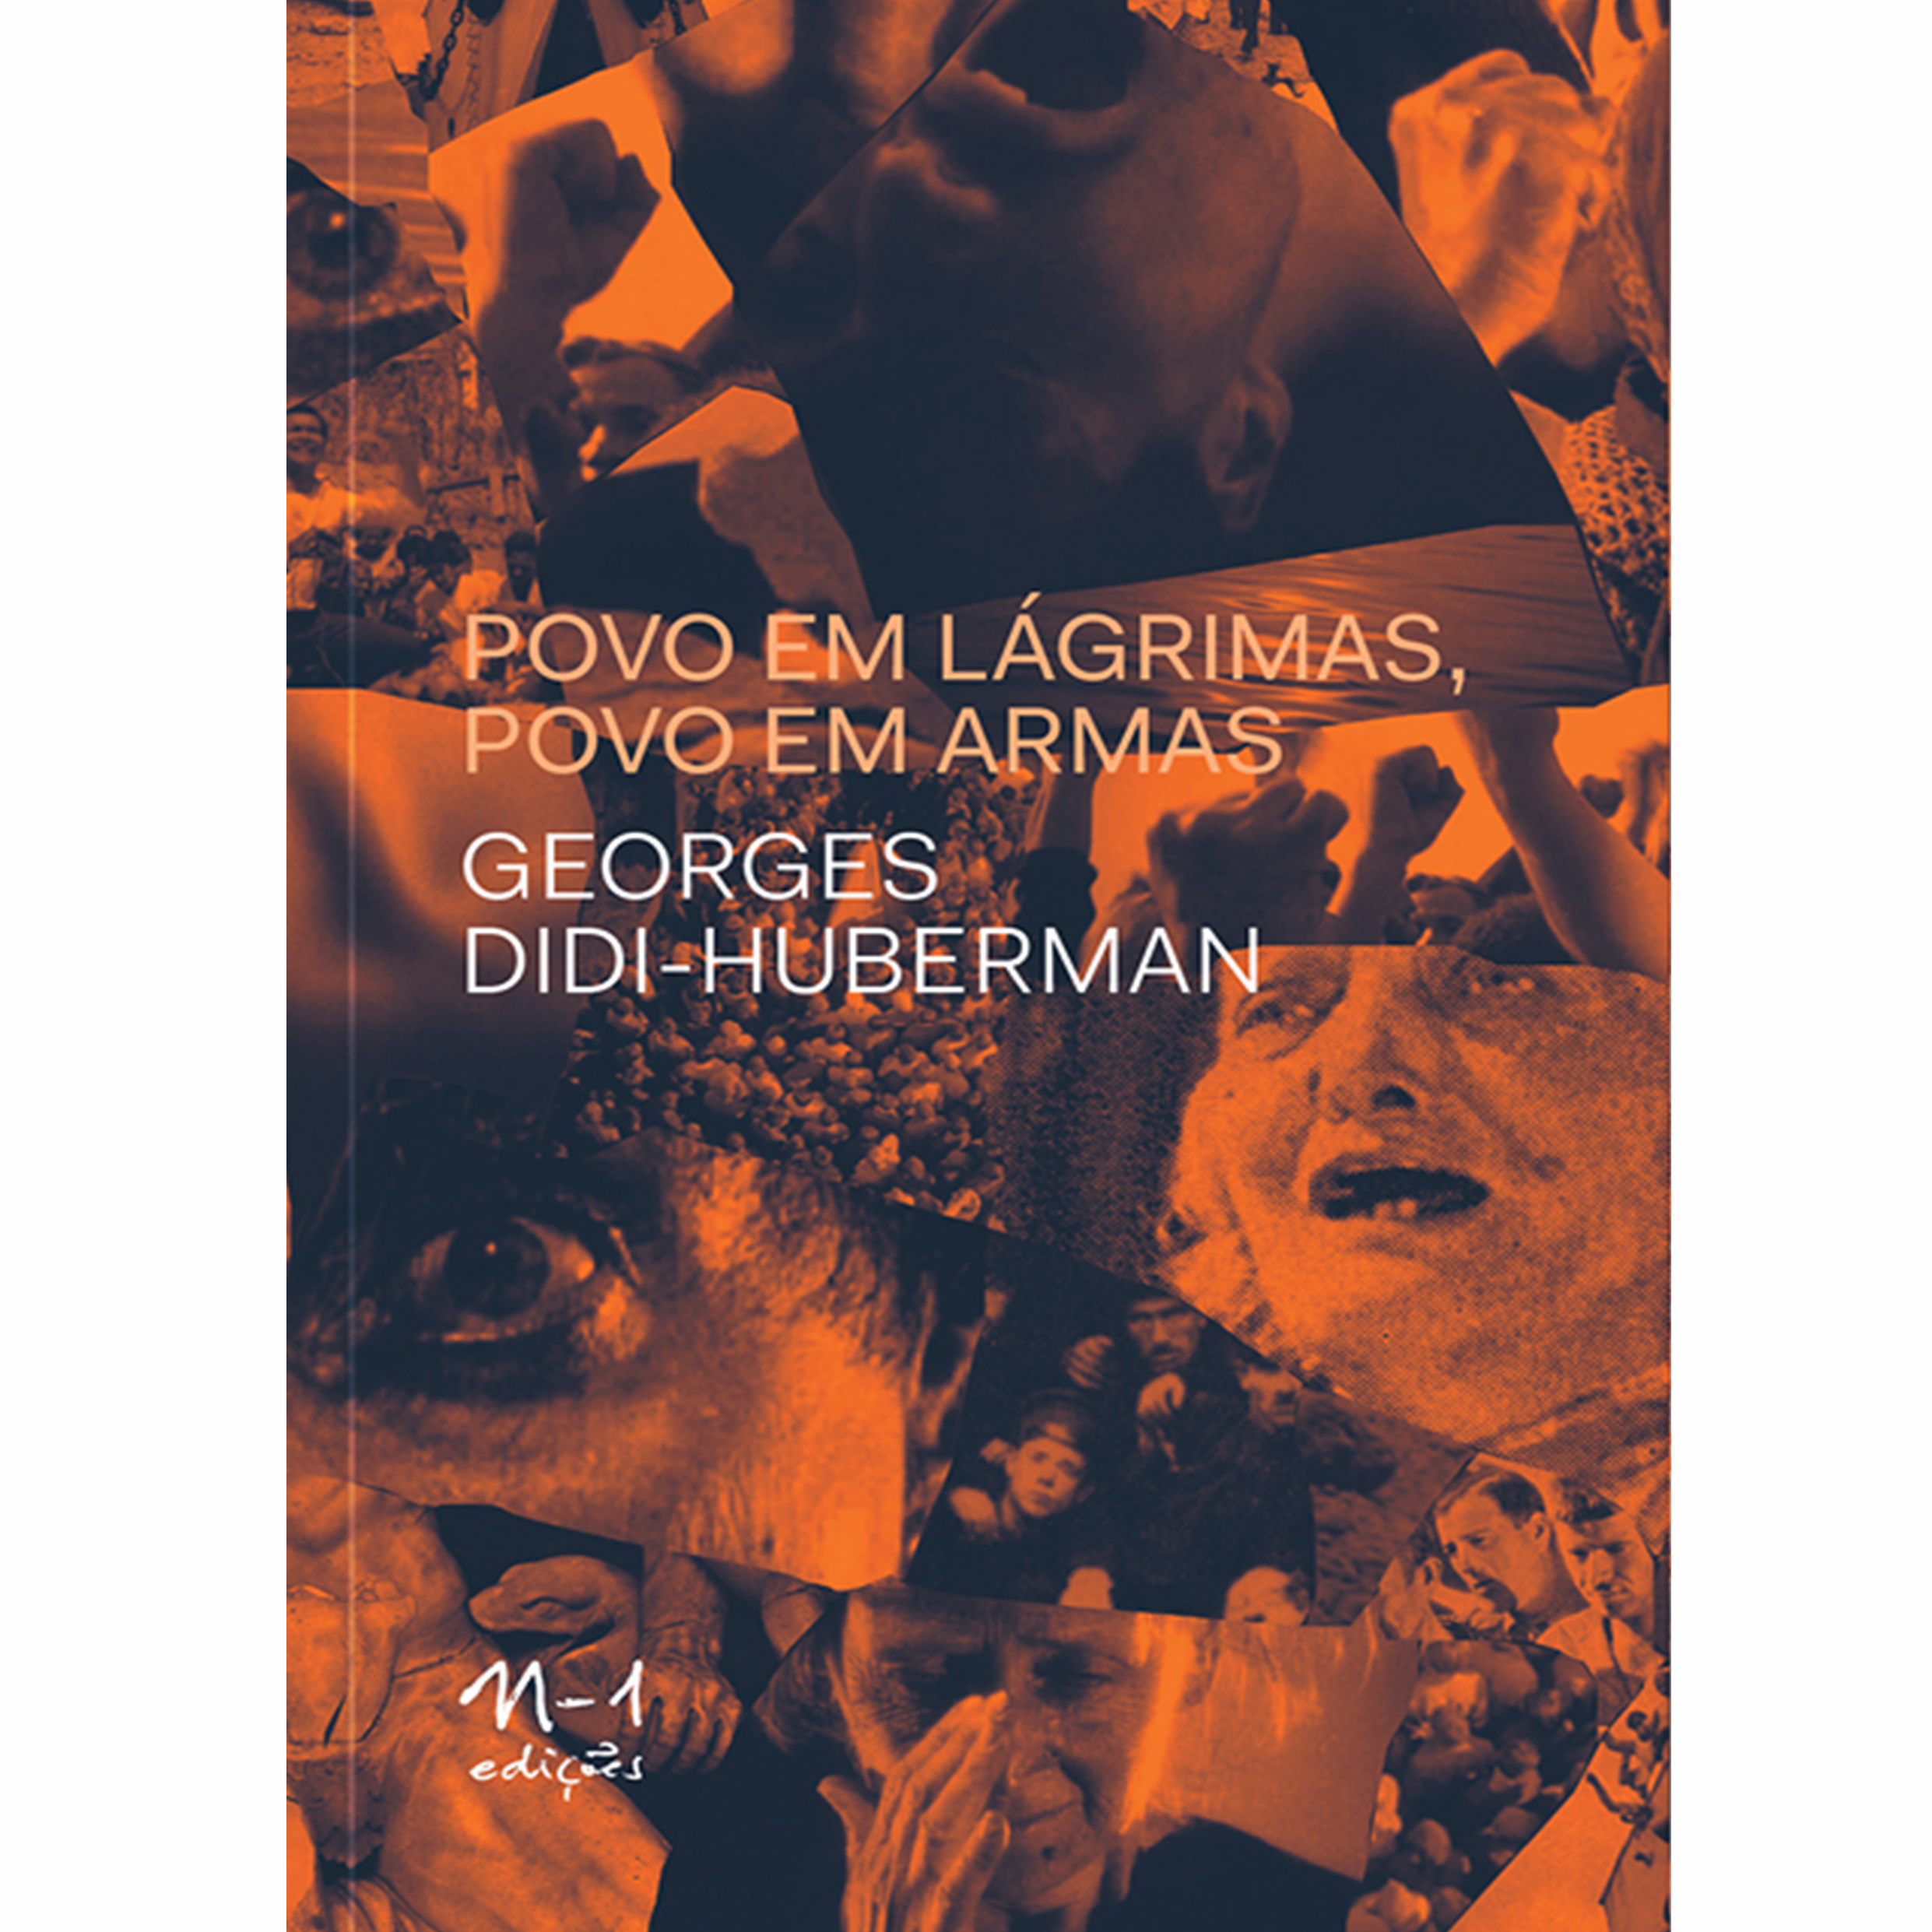
\includegraphics[width=74mm]{./CAPAS/N-1_POVO.jpg}
\end{center}

\hspace*{-7cm}\hrulefill\hspace*{-7cm}

\medskip

\noindent{}Este livro parte da análise de uma única situação, porém exemplar: um homem morre de morte injusta e violenta; mulheres se juntam para chorá-lo; logo mais é um povo em lágrimas que se reúne a elas. Ora, essa situação que se vê por toda parte foi esplendidamente retratada por Serguei Eisenstein em seu célebre filme \textit{O encouraçado Potemkin}. Mas como foi que Roland Barthes, uma das vozes mais influentes no domínio do discurso contemporâneo sobre as imagens, pôde considerar tal construção do \textit{pathos} ``vulgar'' e ``lamentável''?
A melhor resposta à crítica \textit{barthesiana} será fornecida pelo próprio Eisenstein na estrutura de sua sequência de imagens, assim como no discurso --- imenso, abundante, genial, tão importante quanto o dos maiores pensadores de seu tempo --- que ele sustenta sobre a questão das imagens patéticas. Descobre-se uma emoção que sabe dizer \textit{nós}, e não só \textit{eu}, um \textit{pathos} que não é apenas passivo, mas se constitui em \textit{práxis}: \hlc{quando as velhas carpideiras de Odessa, em volta do marinheiro morto, passam da lamentação à cólera, ``prestam queixa'' e exigem justiça, fazem nascer esse \textit{povo em armas} da revolução que vem.}

\vfill

\hspace*{-.4cm}\begin{minipage}[c]{.5\linewidth}
\small\textbf{
\hspace*{-.1cm}Editora: n-1\\
Título: Povo em lágrimas, povo em armas\\
Autor: Georges Didi-Huberman\\ 
ISBN: 978-65-86941-18-0\\
Páginas: 520\\
Formato: 14x21\,cm\\
Preço: R\$ 120,00\\
}
\end{minipage}

\pagebreak

\begin{center}
\hspace*{-3.6cm}\raisebox{5cm}{\rotatebox[origin=t]{90}{\huge\textbf{Lançamento}}}
\hspace*{3.1cm}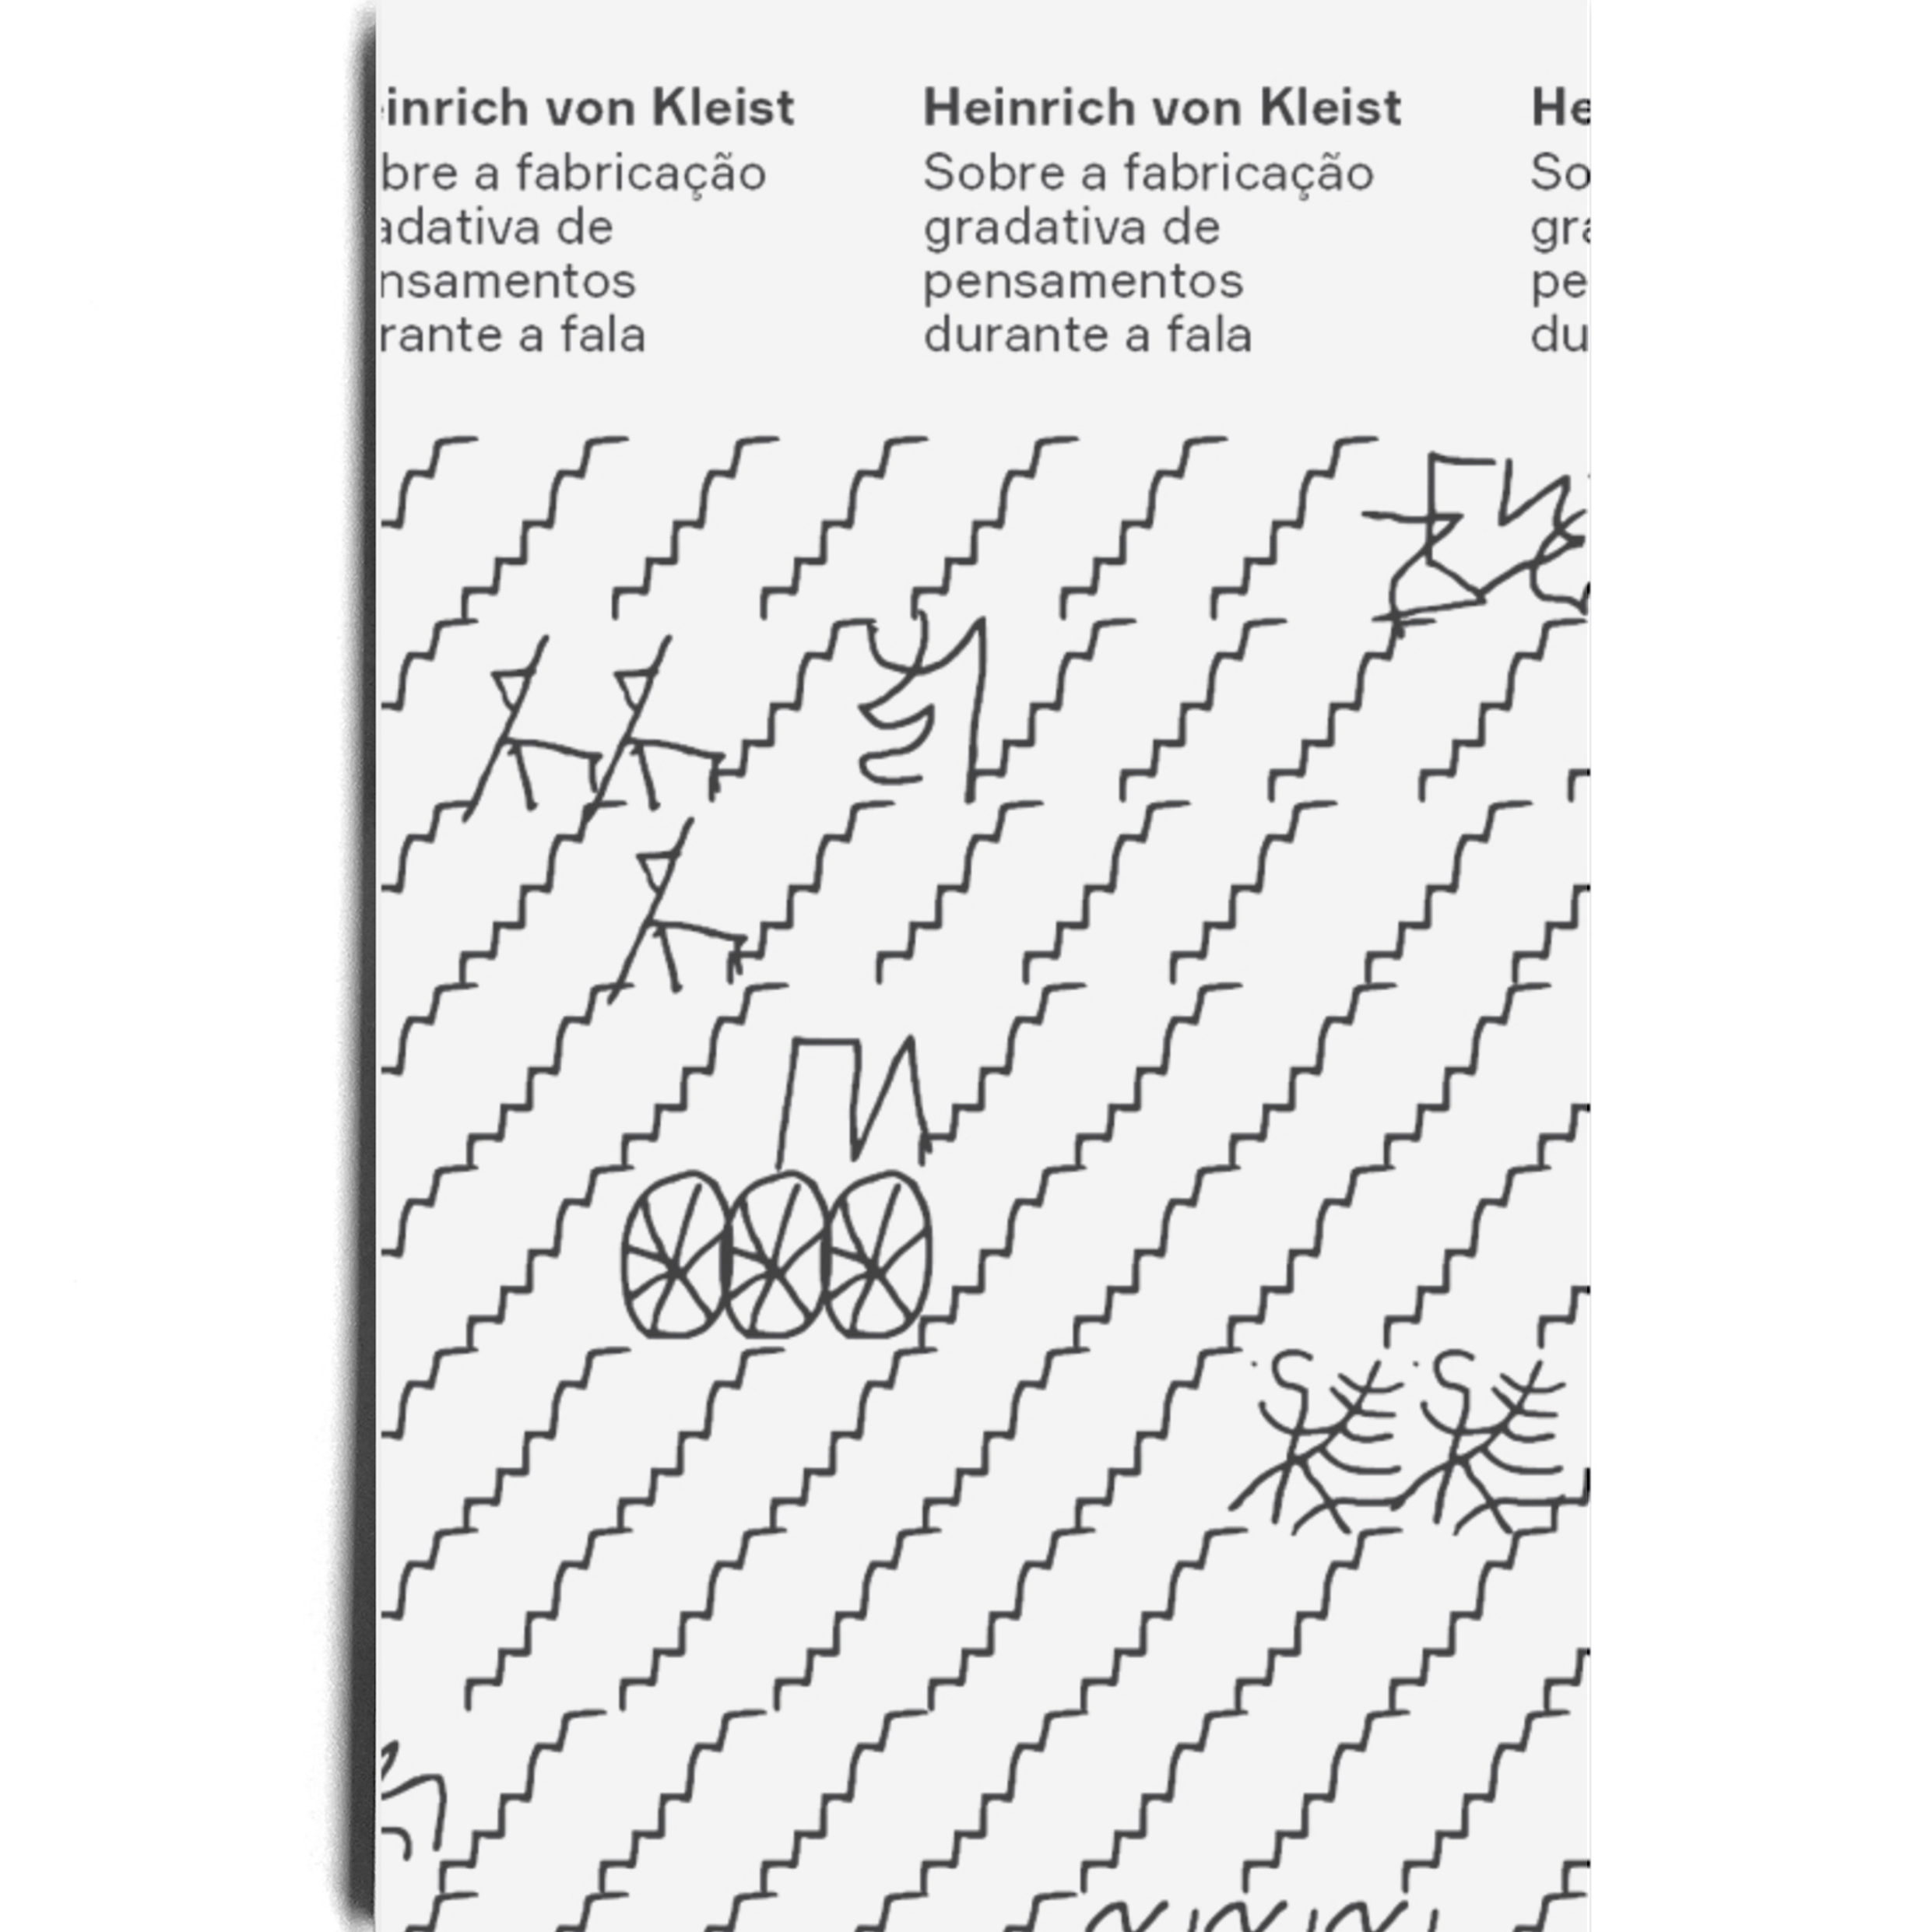
\includegraphics[width=74mm]{./CAPAS/N-1_FABRICACAO.jpg}
\end{center}

\hspace*{-7cm}\hrulefill\hspace*{-7cm}

\medskip

\noindent{}Ensaio publicado por Heinrich von Kleist em 1870, no qual \hlc{aborda a questão da construção do pensamento durante a fala}. Ensaio crítico introdutório de Maria Cristina Franco Ferraz, onde aponta as conexões deste texto com Nietzsche e a extemporaneidade do pensamento, além do pensamento como máquina de guerra proposto por Deleuze e Guattari. 

% Não se alcançam ideias claras isolando-se dos outros e do mundo, em um movimento introspectivo que favoreceria a inspeção da razão por ela mesma. Deleuze e Guattari ressaltam ainda o antiplatonismo dessa espécie de diálogo, que é de fato um anti-diálogo: o texto salienta que começamos a falar com alguém sobre uma ideia nebulosa não para que o interlocutor nos esclareça, mas para que o próprio movimento inicial da frase, infletindo-se em direção a seu desfecho, perfaça e clarifique a ideia. Portanto, nem pensamento interiorizado nem diálogo metódico; em Kleist, não perguntar, apostar na força viva do discurso e no acaso dos encontros faz parte da cena em que o pensamento pode ser fabricado. De fora, portanto, e em trocas presenciais com corpos alheios.


\vfill

\hspace*{-.4cm}\begin{minipage}[c]{.5\linewidth}
\small\textbf{
\hspace*{-.1cm}Editora: n-1 \& Hedra\\
Título: Sobre a fabricação gradativa de pensamentos durante a fala\\
Autor: Heinrich von Kleist\\ 
ISBN: 978-65-86941-44-9\\
Páginas: 80\\
Formato: 18x11\,cm\\
Preço: R\$ 36,00\\
}
\end{minipage}

\pagebreak

\begin{center}
\hspace*{.5cm}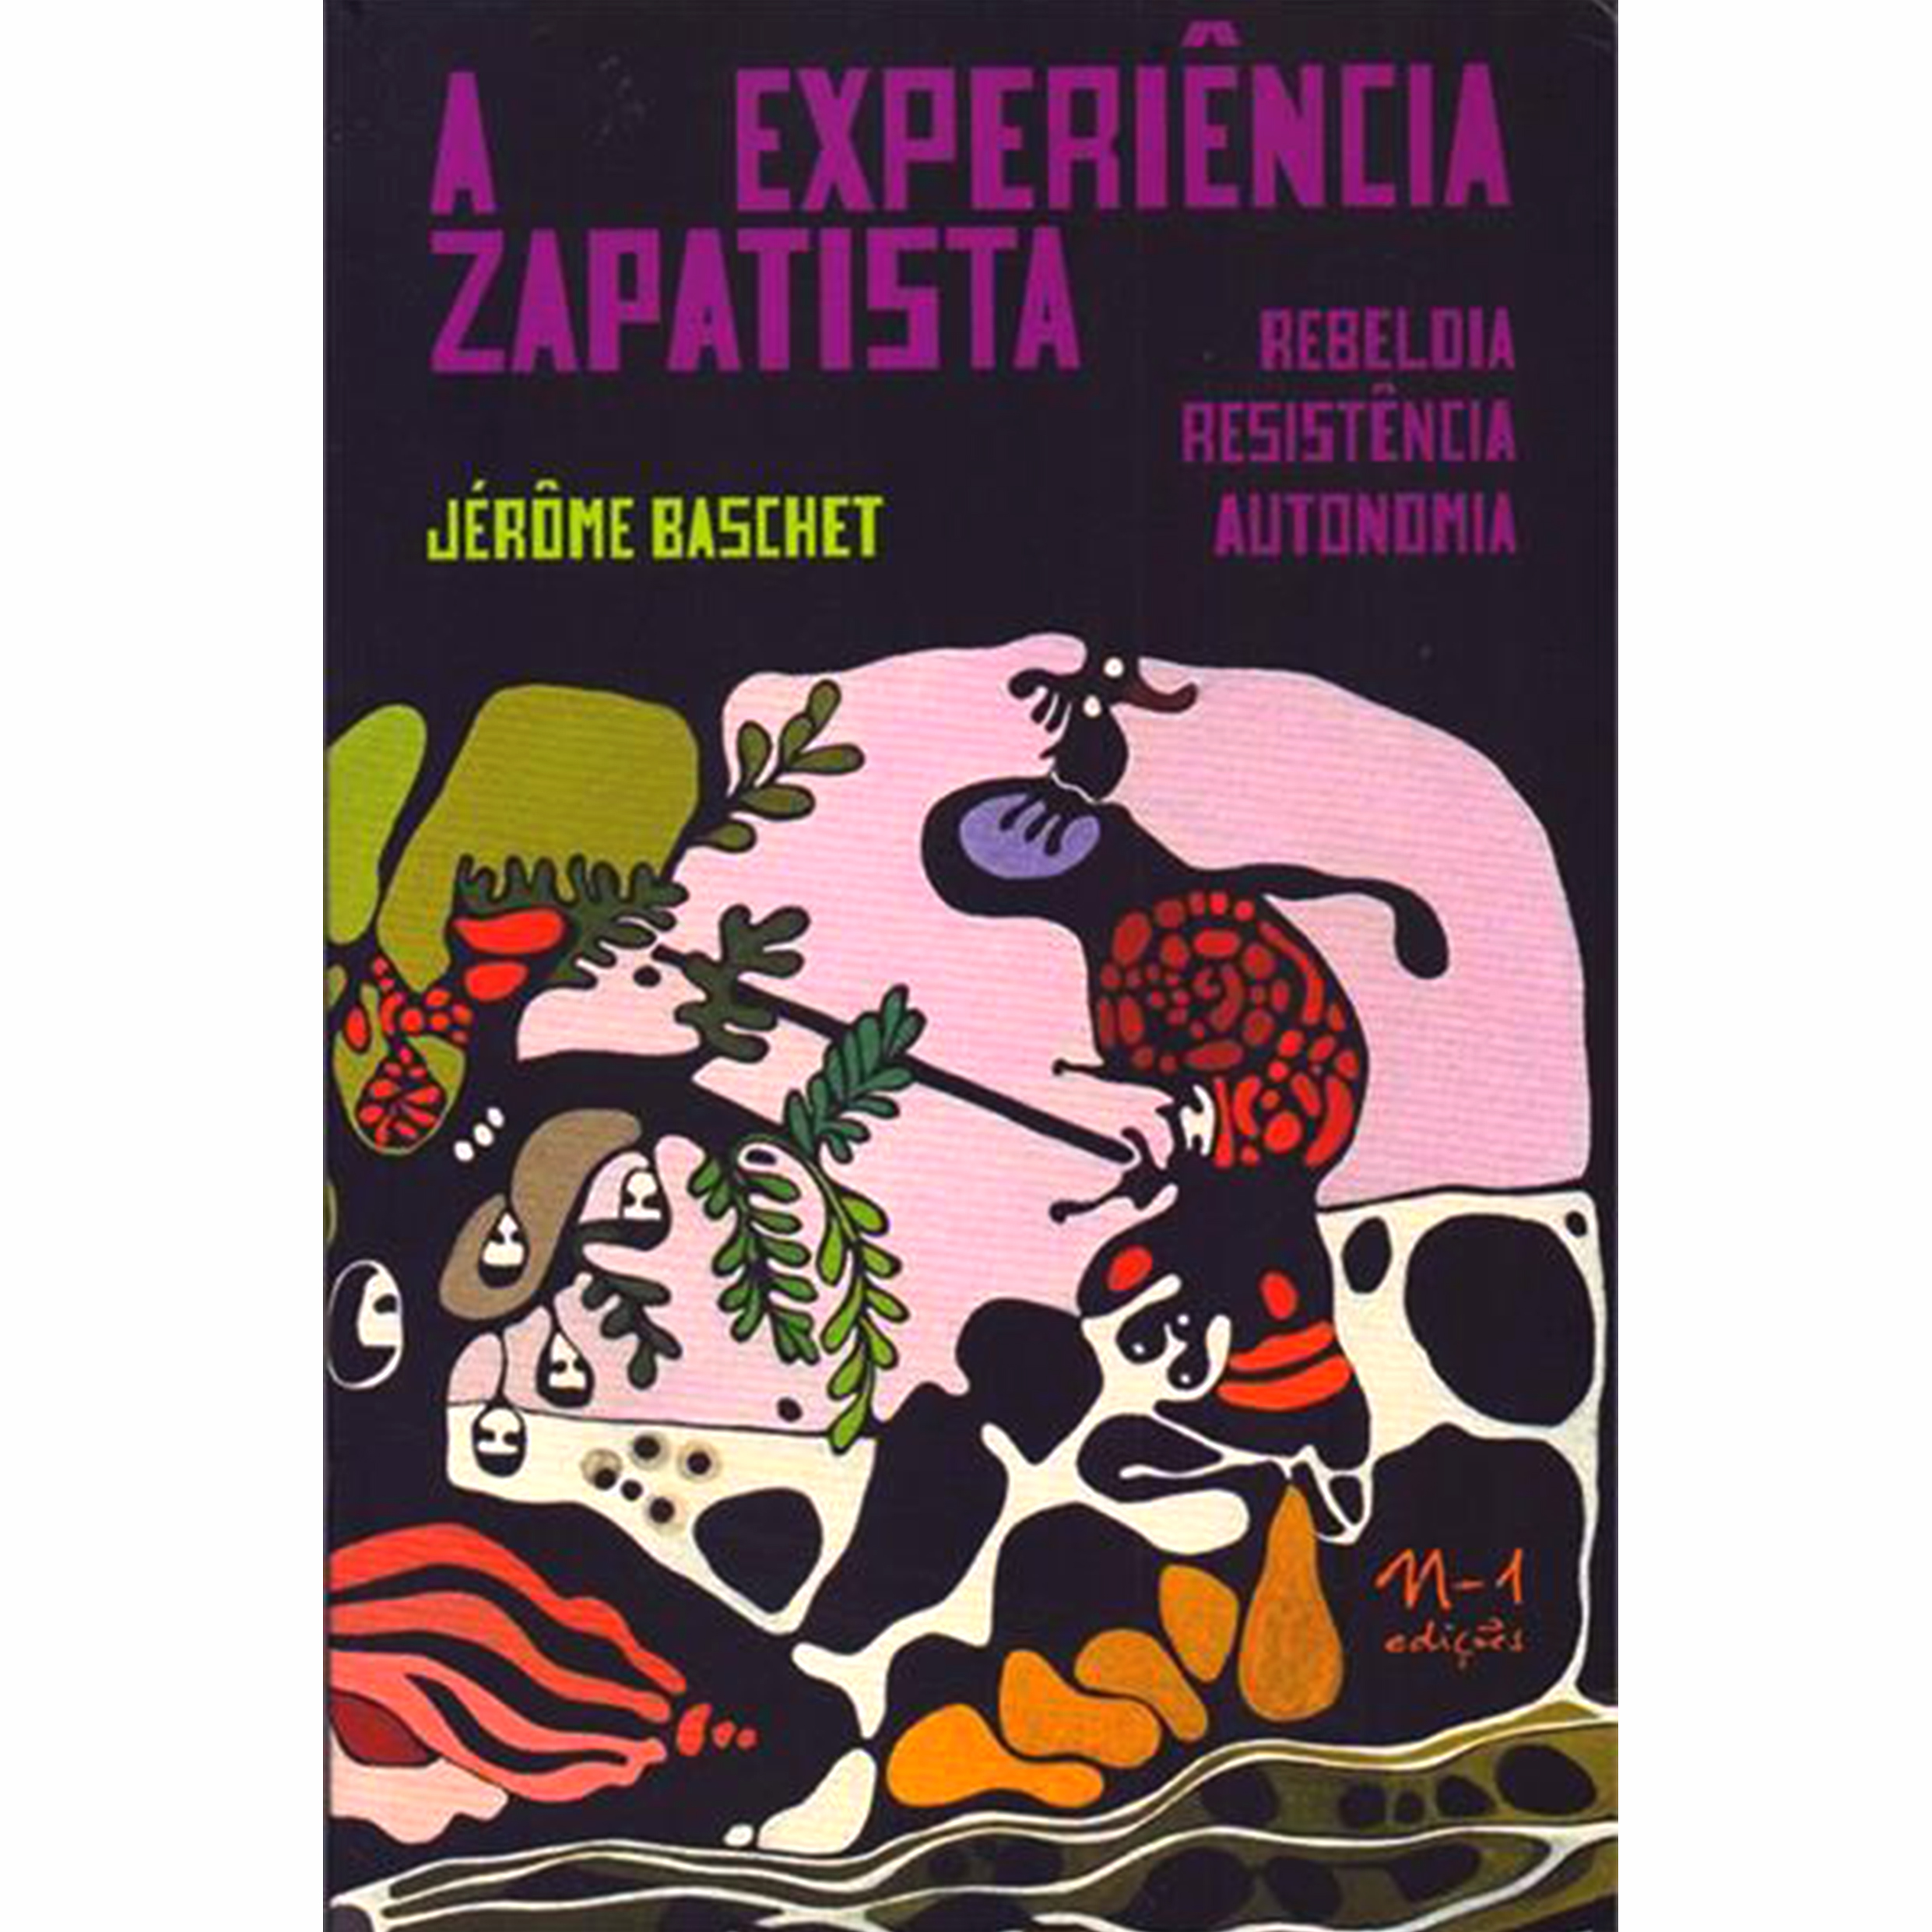
\includegraphics[width=74mm]{./CAPAS/N-1_EXPERIENCIA.jpg}
\end{center}

\hspace*{-7cm}\hrulefill\hspace*{-7cm}

\medskip

\noindent{}``É nossa convicção e nossa prática que para se rebelar e lutar não são necessários nem líderes, nem caudilhos, nem messias, nem salvadores. Para lutar é necessário apenas um pouco de vergonha, um tanto de dignidade e muita organização'', escreveu o Subcomandante Marcos, em 2014. Neste livro, \hlc{o historiador Jérôme Baschet retraça a gênese do movimento zapatista e reconstitui suas várias etapas, desde o levante armado até os dias de hoje}. Assim, temos acesso à lógica de sua organização, à capacidade de autotransformação e à originalidade de sua trajetória. O prefácio do autor acrescido à edição brasileira nos inspira a atravessar a noite tão escura no Brasil à luz da experiência zapatista, que é também indígena, feminina, e poética.

\vfill

\hspace*{-.4cm}\begin{minipage}[c]{.5\linewidth}
\small\textbf{
\hspace*{-.1cm}Editora: n-1\\
Título: A experiência zapatista\\
Autor: Jerôme Baschet\\
ISBN: 978-65-86941-41-8\\
Páginas: 400\\
Formato: 14x21\,cm\\
Preço: R\$ 100,00\\
}
\end{minipage}

\pagebreak

\pagebreak

\begin{center}
\hspace*{-3.6cm}\raisebox{5cm}{\rotatebox[origin=t]{90}{\huge\textbf{Lançamento}}}
\hspace*{3.1cm}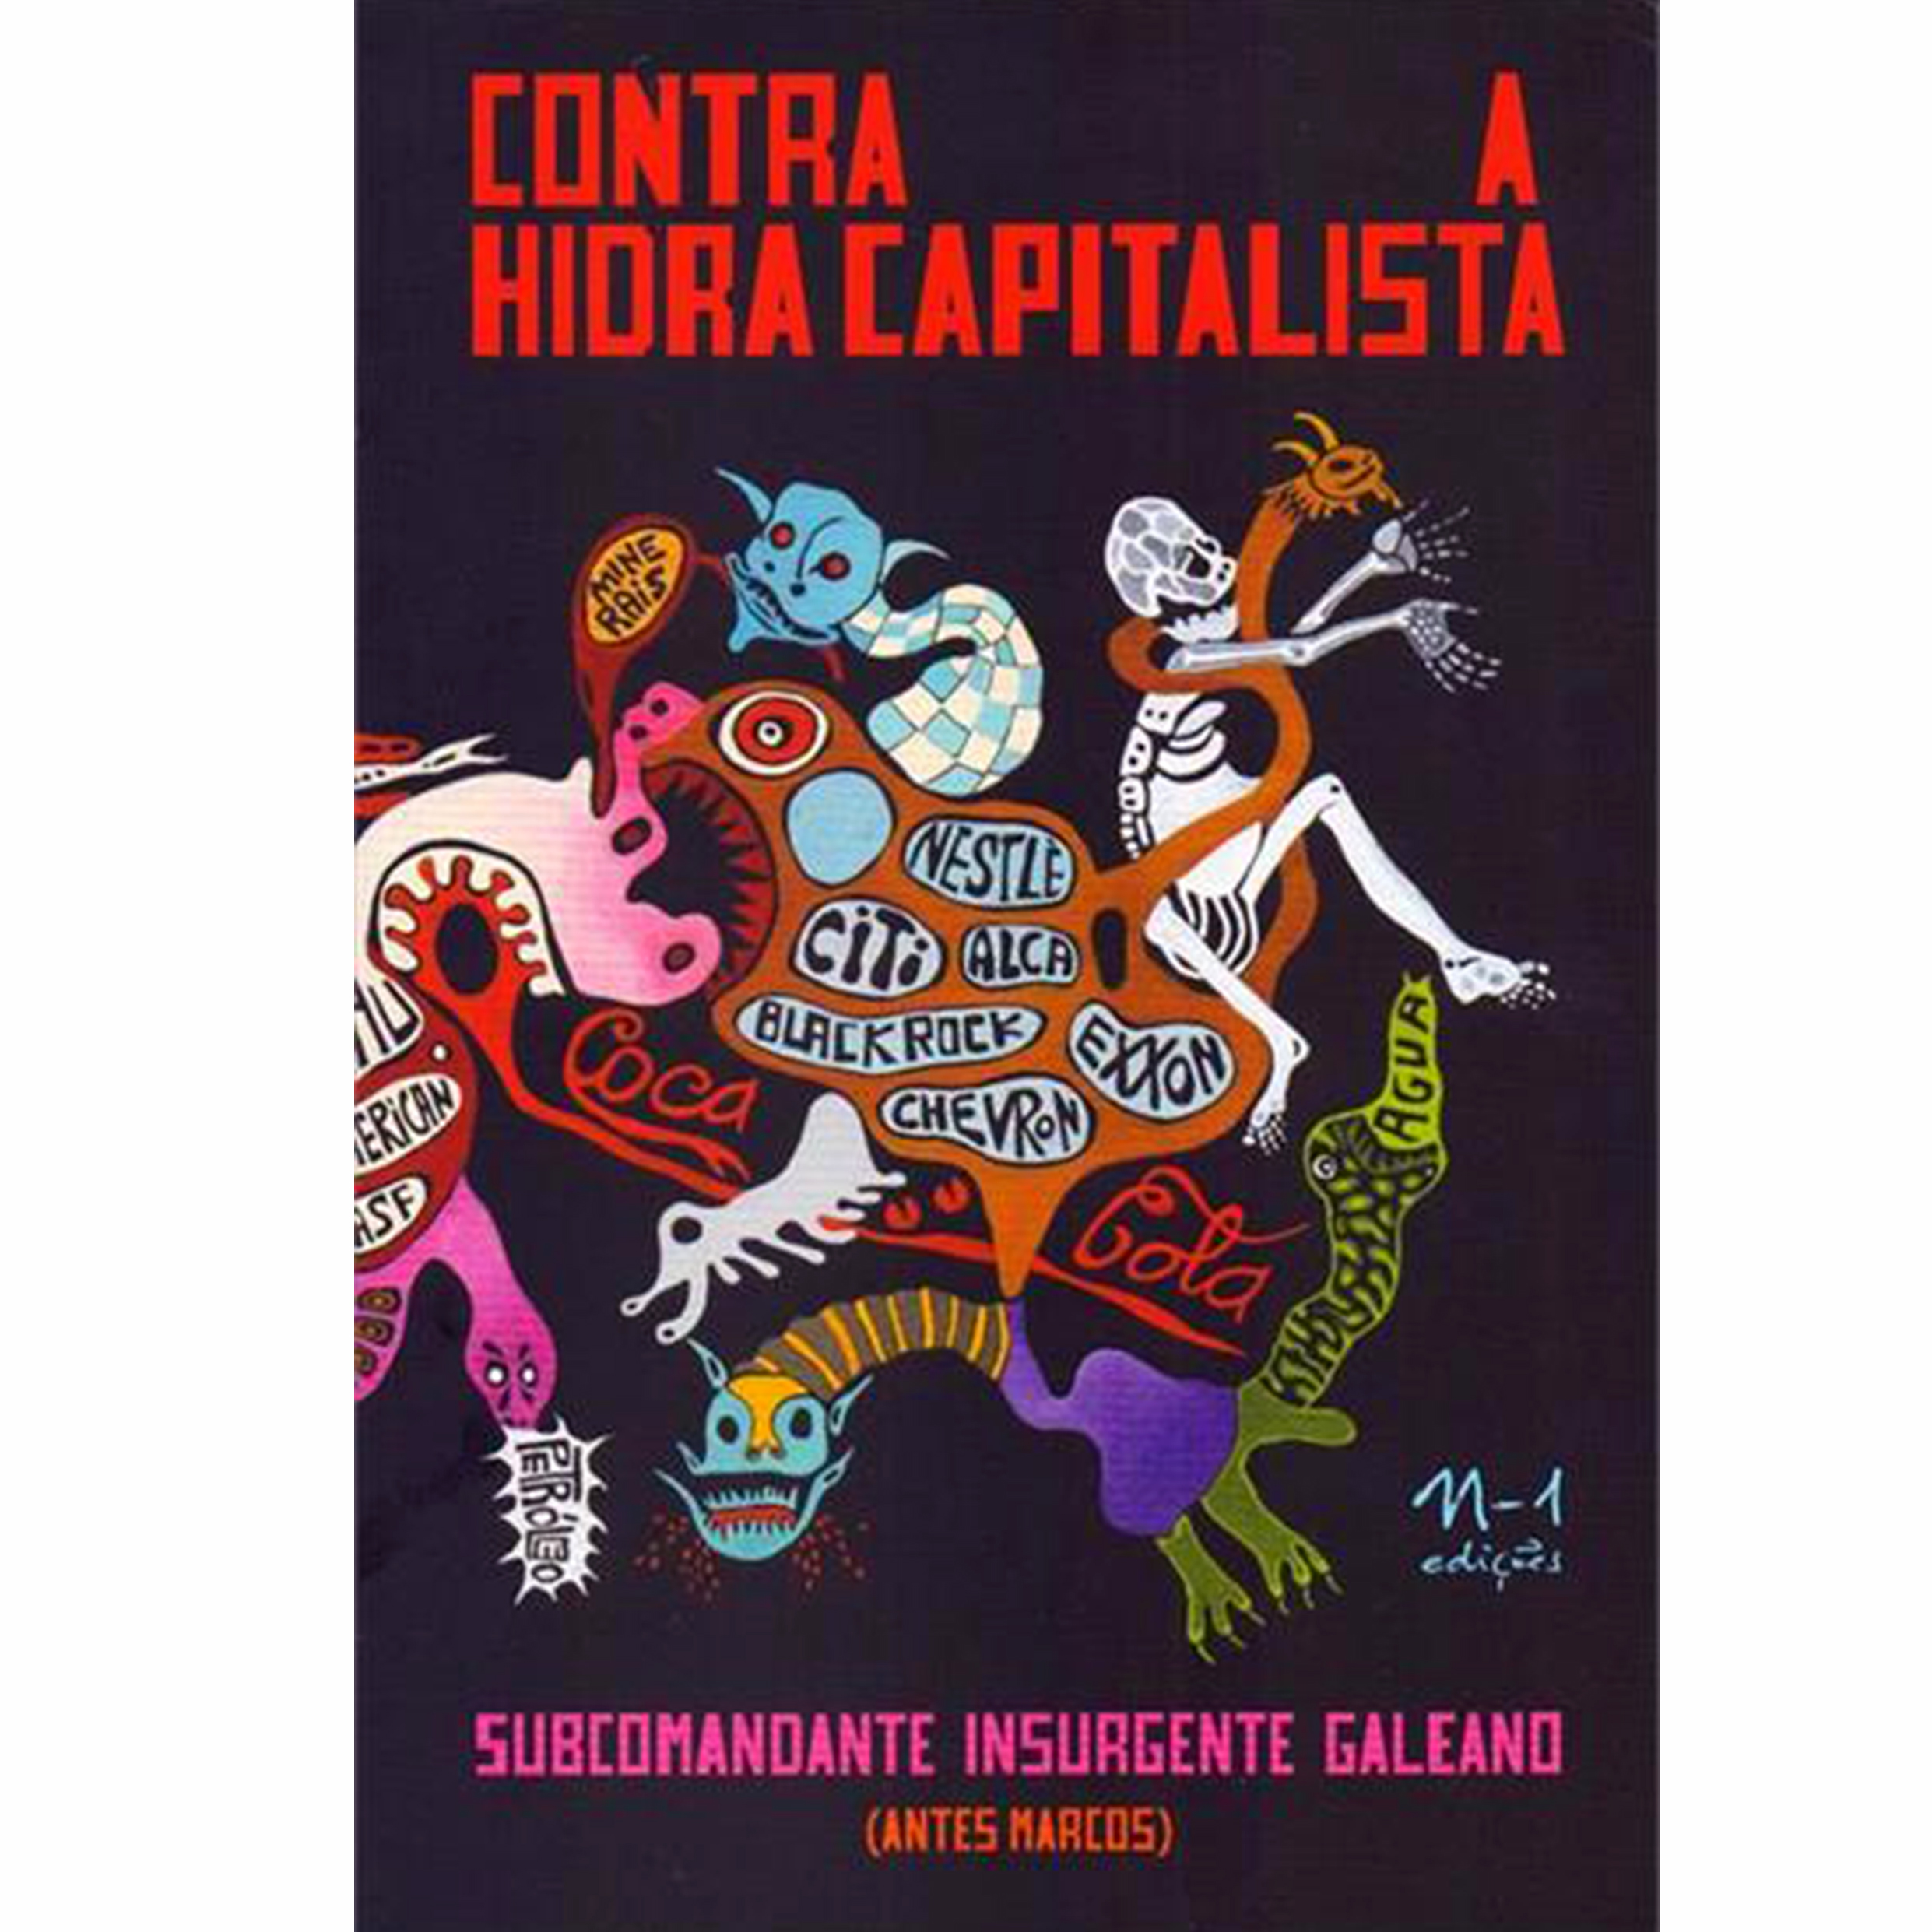
\includegraphics[width=74mm]{./CAPAS/N-1_HIDRA.jpg}
\end{center}

\hspace*{-7cm}\hrulefill\hspace*{-7cm}

\medskip

\noindent{}Para além da aura midiática do encapuzado Subcomandante Insurgente Marcos, rebatizado de Galeano em 2014, \hlc{quase nada sabemos das motivações, aspirações, estratégias e rumos dessa insurgência que desde 1994 ocupa parte do território mexicano. No entanto, ali surgiu um dos bolsões revolucionários mais originais deste século}. Liberados da obsessão estatista, da lógica capitalista, da propriedade privada da terra, da dominação de gênero, de etnia, de classe --- eis uma insurgência que reverteu a mercantilização da existência. Quem melhor do que aquele que a liderou, em seu estilo jocoso, elíptico, à beira da ficção, para dá-la a ver? \textit{Contra a Hidra Capitalista}, com falas do Subcomandante Insurgente Galeano, é um dos quatro livros desta coleção zapatista. Os outros são \textit{A experiência zapatista: rebeldia, resistência e autonomia}, por Jérôme Baschet, \textit{Uma baleia na montanha}, por Mariana Lacerda e Peter Pál Pelbart, e \textit{Mensagens revolucionárias}, por Antonin Artaud. As pinturas das capas dos livros são de Rivane Neuenschwander.

\vfill

\hspace*{-.4cm}\begin{minipage}[c]{.5\linewidth}
\small\textbf{
\hspace*{-.1cm}Editora: n-1\\
Título: Contra a hidra capitalista\\
Autor: Subcomandante Marcos Galeano\\ 
ISBN: 978-65-86941-42-5\\
Páginas: 192\\
Formato: 14x21\,cm\\
Preço: R\$ 70,00\\
}
\end{minipage}

\pagebreak

\begin{center}
\hspace*{.5cm}
\includegraphics[width=74mm]{./CAPAS/N-1_DEVIR.jpg}
\end{center}

\hspace*{-7cm}\hrulefill\hspace*{-7cm}

\medskip

\noindent{}Itziar Ziga conhece a cidade como quem sempre viveu fora. Anda pelas ruas como se pertencessem a ela. Sapatos de princesinha, mas com as solas desgastadas. Dá pra perceber que já fez todos os trajetos, tanto de noite quanto de dia, tanto alerta quanto doidona, com os olhos cheios de lágrimas ou de raiva, em grupo, casal, trisal, sozinha, mas sempre parte da matilha. Mulher da rua, garota de bar, rata de livrarias e corredora de manifestações. \hlc{Itziar Ziga é uma mistureba político-cultural: o campo e a cidade, sua mãe e suas colegas, Euskalerria e Catalunya, o melô e o feminismo iraquiano, Judith Butler e Manuela Trasobares, a teoria queer e as oficinas de pantojismo, a cultura trans e as avós putas, Alaska e Benedetti, santa Ágata e a Dulce Neus}. (Trecho do prefácio de Paul B. Preciado e Virginie Despentes.)

\vfill

\hspace*{-.4cm}\begin{minipage}[c]{.5\linewidth}
\small\textbf{
\hspace*{-.1cm}Editora: n-1\\
Título: Devir cachorra\\
Autor: Itziar Ziga\\
ISBN: 978-65-86941-47-0\\
Páginas: 176\\
Formato: 14x21\,cm\\
Preço: R\$ 54,00\\
}
\end{minipage}

\pagebreak

\begin{center}
\hspace*{-3.6cm}\raisebox{5cm}{\rotatebox[origin=t]{90}{\huge\textbf{Lançamento}}}
\hspace*{3.1cm}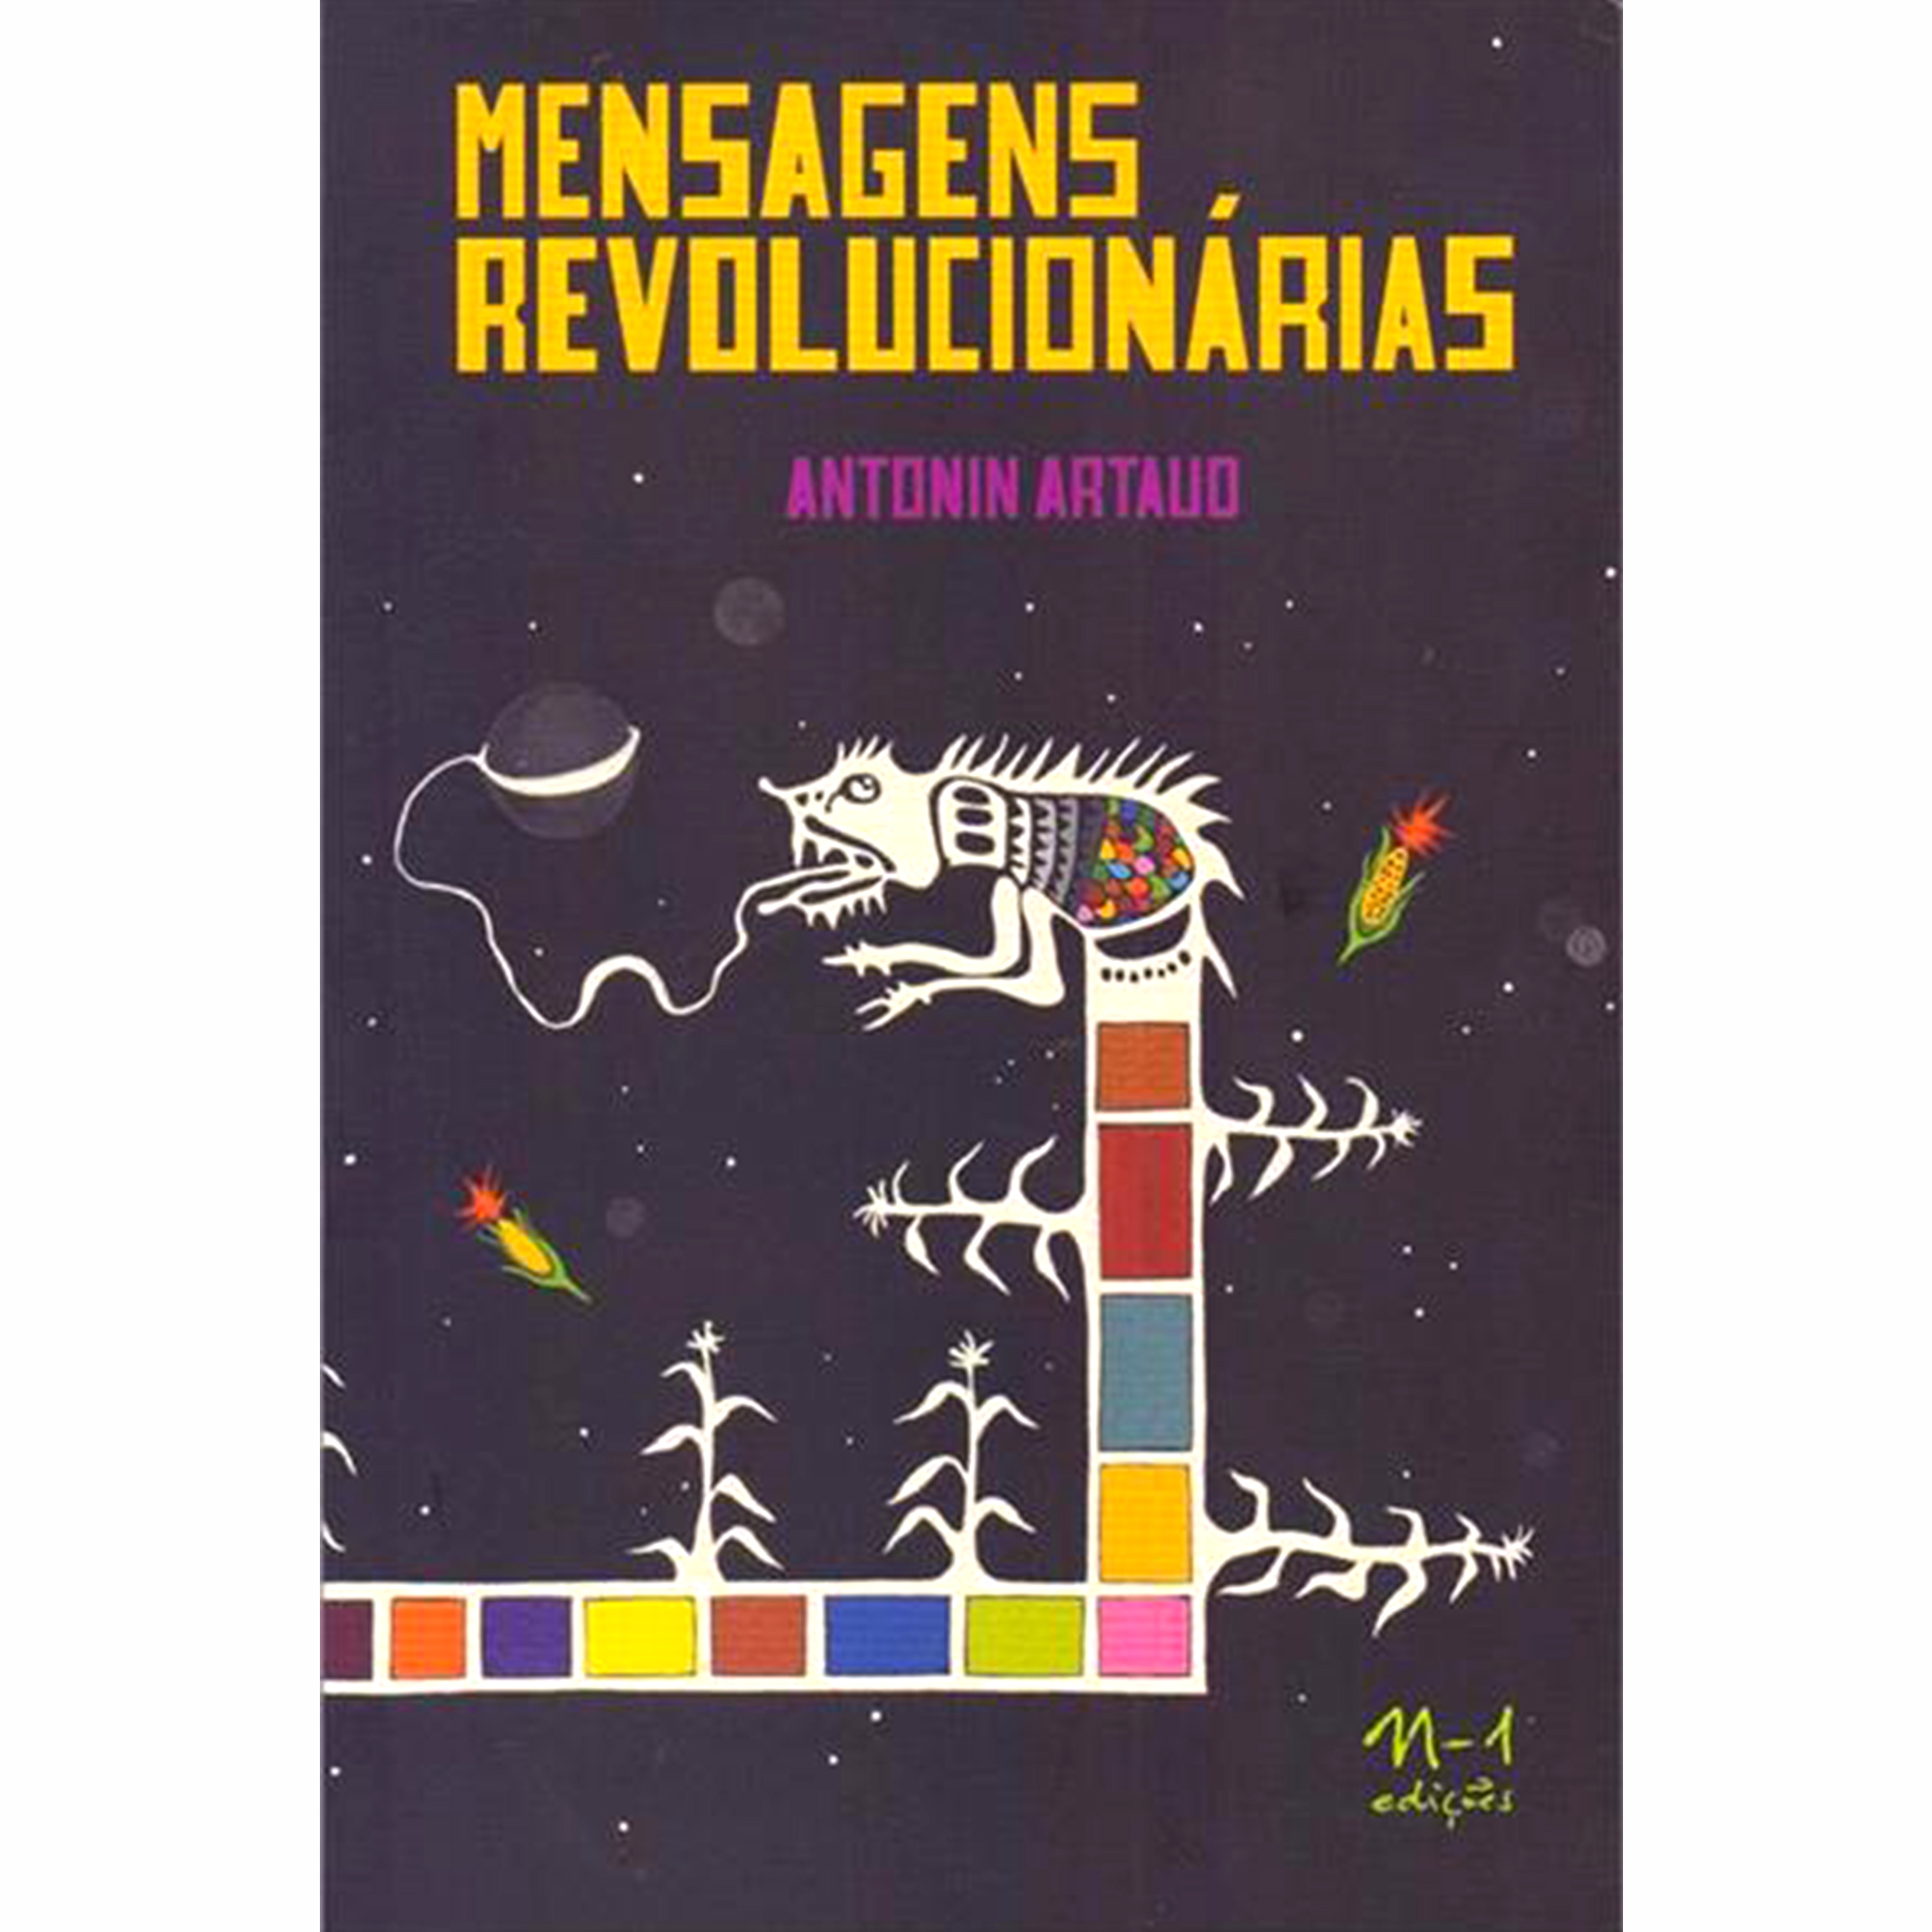
\includegraphics[width=74mm]{./CAPAS/N-1_MENSAGENS.jpg}
\end{center}

\hspace*{-7cm}\hrulefill\hspace*{-7cm}

\medskip

\noindent{}Os textos, conferências e artigos aqui reunidos são fruto da estadia de Antonin Artaud no México, ocorrida em 1936. Mas afinal, o que Artaud foi fazer no México? É esta pergunta que acompanha a mente de quem percorre esses \textit{manifestos} sulfurosos. Eis a resposta do autor: \hlc{``Junto à revolução social e econômica indispensável, esperamos todos uma revolução da consciência que nos permitirá curar a vida. Cabe ao México moderno empreender essa revolução} (...) Nós esperamos do México, em suma, um novo conceito de revolução (...) e também um novo conceito do Homem''. Nesta frase encontramos a semente que nos inspira a avizinhar textos deixados por Artaud ao Movimento Zapatista.

\vfill

\hspace*{-.4cm}\begin{minipage}[c]{.5\linewidth}
\small\textbf{
\hspace*{-.1cm}Editora: n-1\\
Título: Mensagens revolucionárias\\
Autor: Antonin Artaud\\ 
ISBN: 978-65-86941-53-1\\
Páginas: 112\\
Formato: 14x21cm\\
Preço: R\$ 60,00\\
}
\end{minipage}

\pagebreak

\begin{center}
\hspace*{.5cm}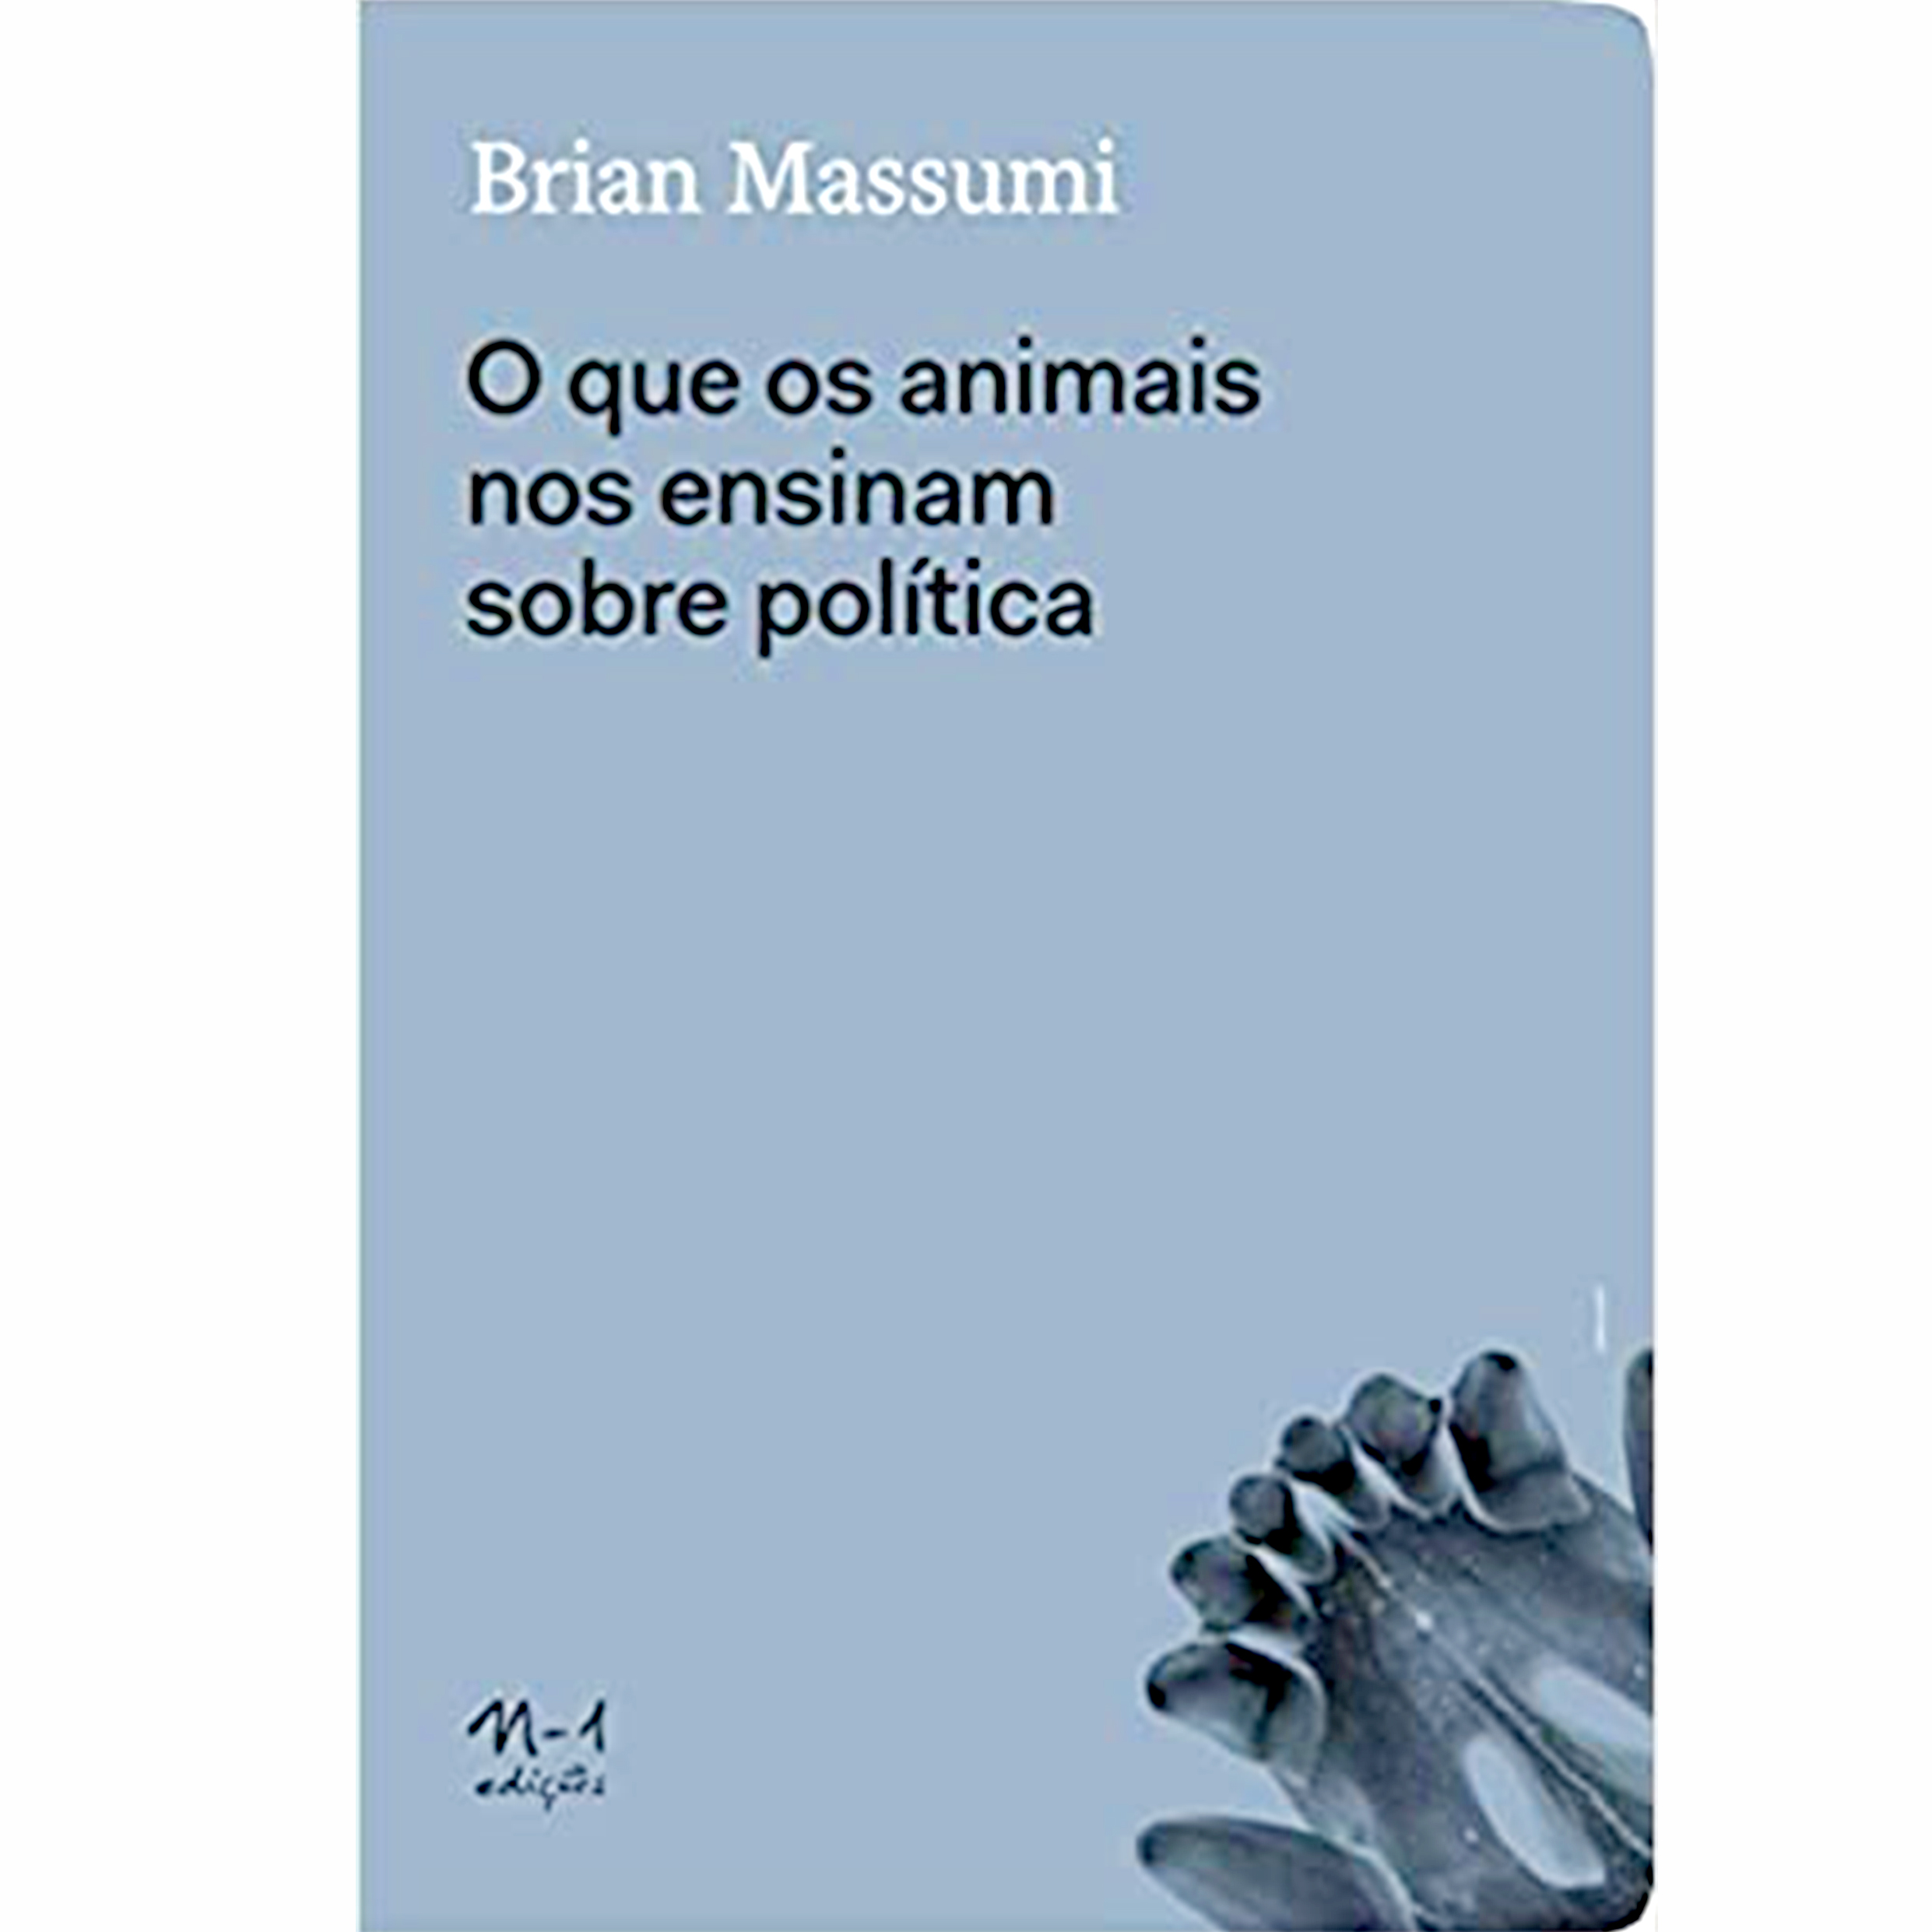
\includegraphics[width=74mm]{./CAPAS/N-1_ANIMAIS.jpg}
\end{center}

\hspace*{-7cm}\hrulefill\hspace*{-7cm}

\medskip

\noindent{} Em \textit{O que os animais nos ensinam sobre política}, \hlc{o filósofo canadense Brian Massumi discute a questão do animal sob uma ótica inusitada. Noções tais como jogo, simpatia e criatividade, menosprezadas pela biologia evolucionista}, pelas ciências do comportamento animal ou pela filosofia, aqui são diretamente incorporadas ao conceito de natureza.

\vfill

\hspace*{-.4cm}\begin{minipage}[c]{.5\linewidth}
\small\textbf{
\hspace*{-.1cm}Editora: n-1\\
Título: O que os animais nos ensinam\\sobre política\\
Autor: Brian Mussumi\\
ISBN: 978-85-66943-47-4\\
Páginas: 192\\
Formato: 14x21\,cm\\
Preço: R\$ 55,00\\
}
\end{minipage}

\pagebreak

\begin{center}
\hspace*{-3.6cm}\raisebox{5cm}{\rotatebox[origin=t]{90}{\huge\textbf{Lançamento}}}
\hspace*{3.1cm}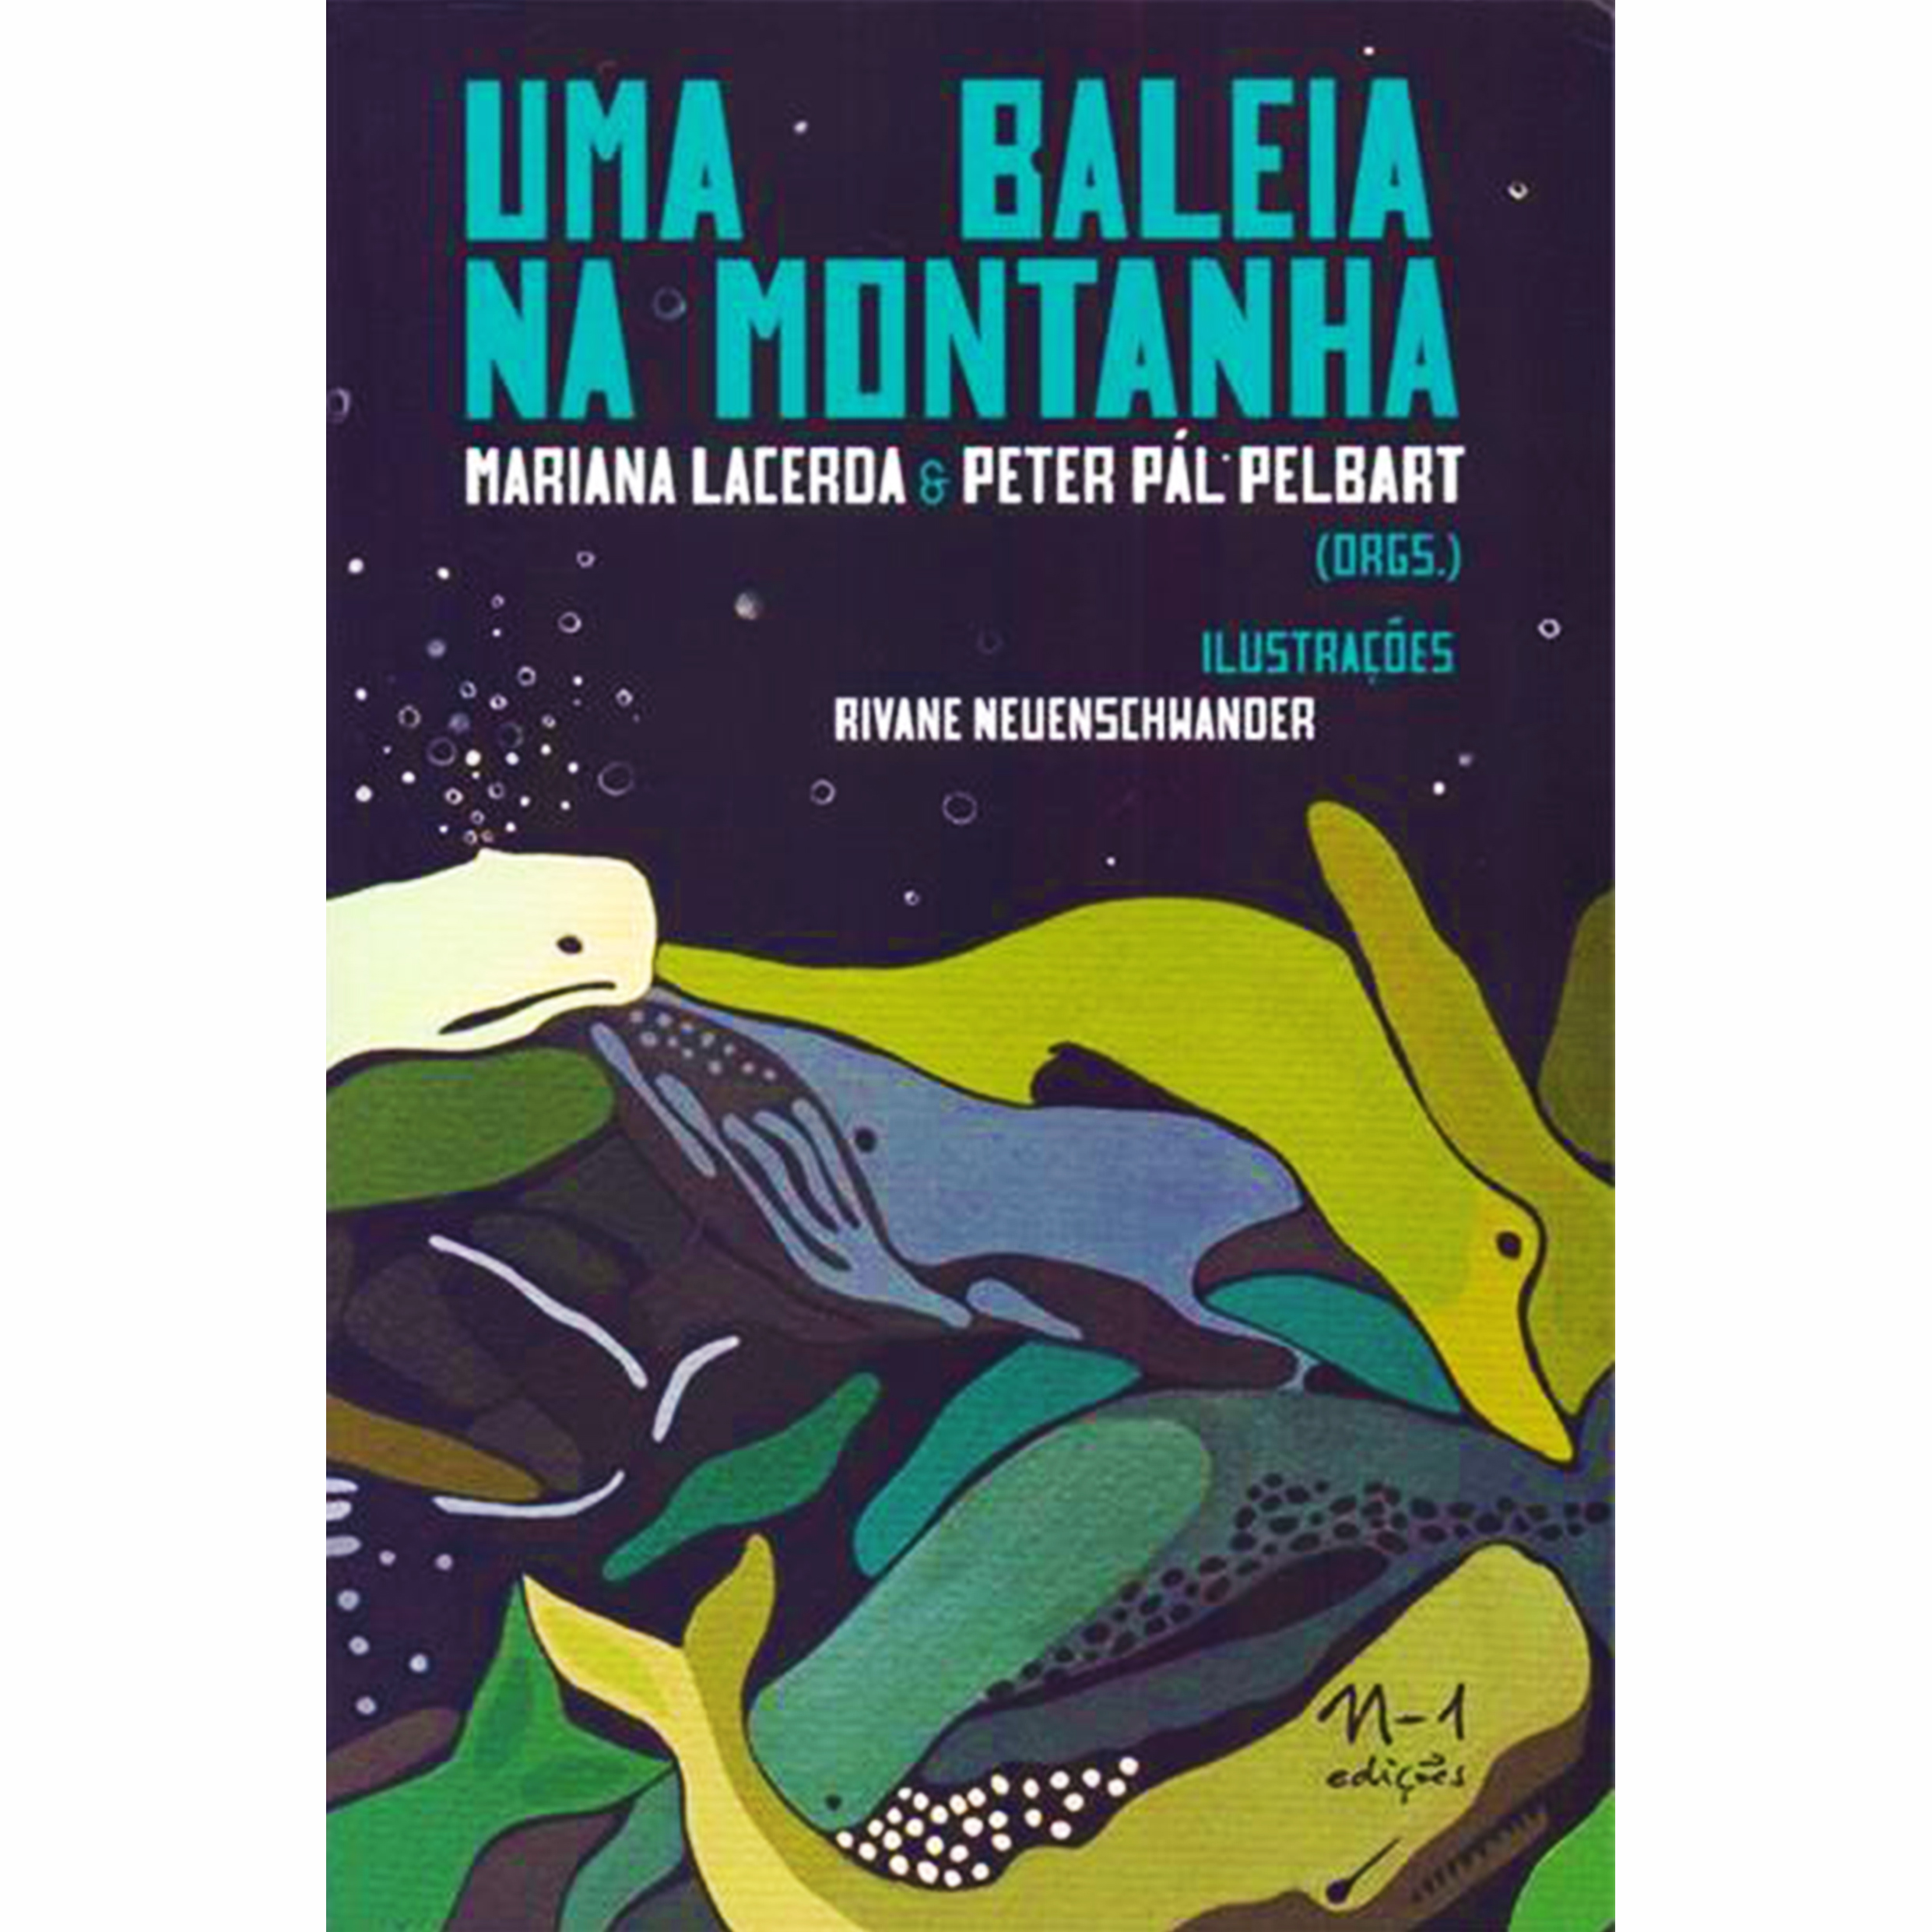
\includegraphics[width=74mm]{./CAPAS/N-1_BALEIA.jpg}
\end{center}

\hspace*{-7cm}\hrulefill\hspace*{-7cm}

\medskip

\noindent{}Para além de certos clichês, \hlc{pouco se sabe sobre o zapatismo no Brasil. Um movimento que parece ter surgido do nada, e às portas do terceiro milênio pega em armas, não para ensejar a militarização da luta, mas ao contrário, para chegar ao ponto em que se possa prescindir delas}. Um movimento que desmonetariza as trocas, rejeita a subserviência ao Estado e ao Capital, e a partir da herança maia reinventa as práticas comuns e as faz colocando a natureza, as mulheres, gays, trans e crianças no centro de seu mundo, sustentando o que os gregos chamavam de parrhesia, a palavra franca, o dizer-verdadeiro; para os maia: a \textit{palavra-espelho}. Um conto infantil do Subcomandante Marcos, com pinturas de Rivane Neuenschwander, é um convite especial às nossas crianças cujas almas parecem tão cansadas de telas.

\vfill

\hspace*{-.4cm}\begin{minipage}[c]{.5\linewidth}
\small\textbf{
\hspace*{-.1cm}Editora: n-1\\
Título: Uma baleia na montanha\\
Autor: Subcomandante Marcos\\ 
ISBN: 978-65-86941-32-6\\
Páginas: 288\\
Formato: 14x21cm\\
Preço: R\$ 87,00\\
}
\end{minipage}

\pagebreak

\begin{center}
\hspace*{.5cm}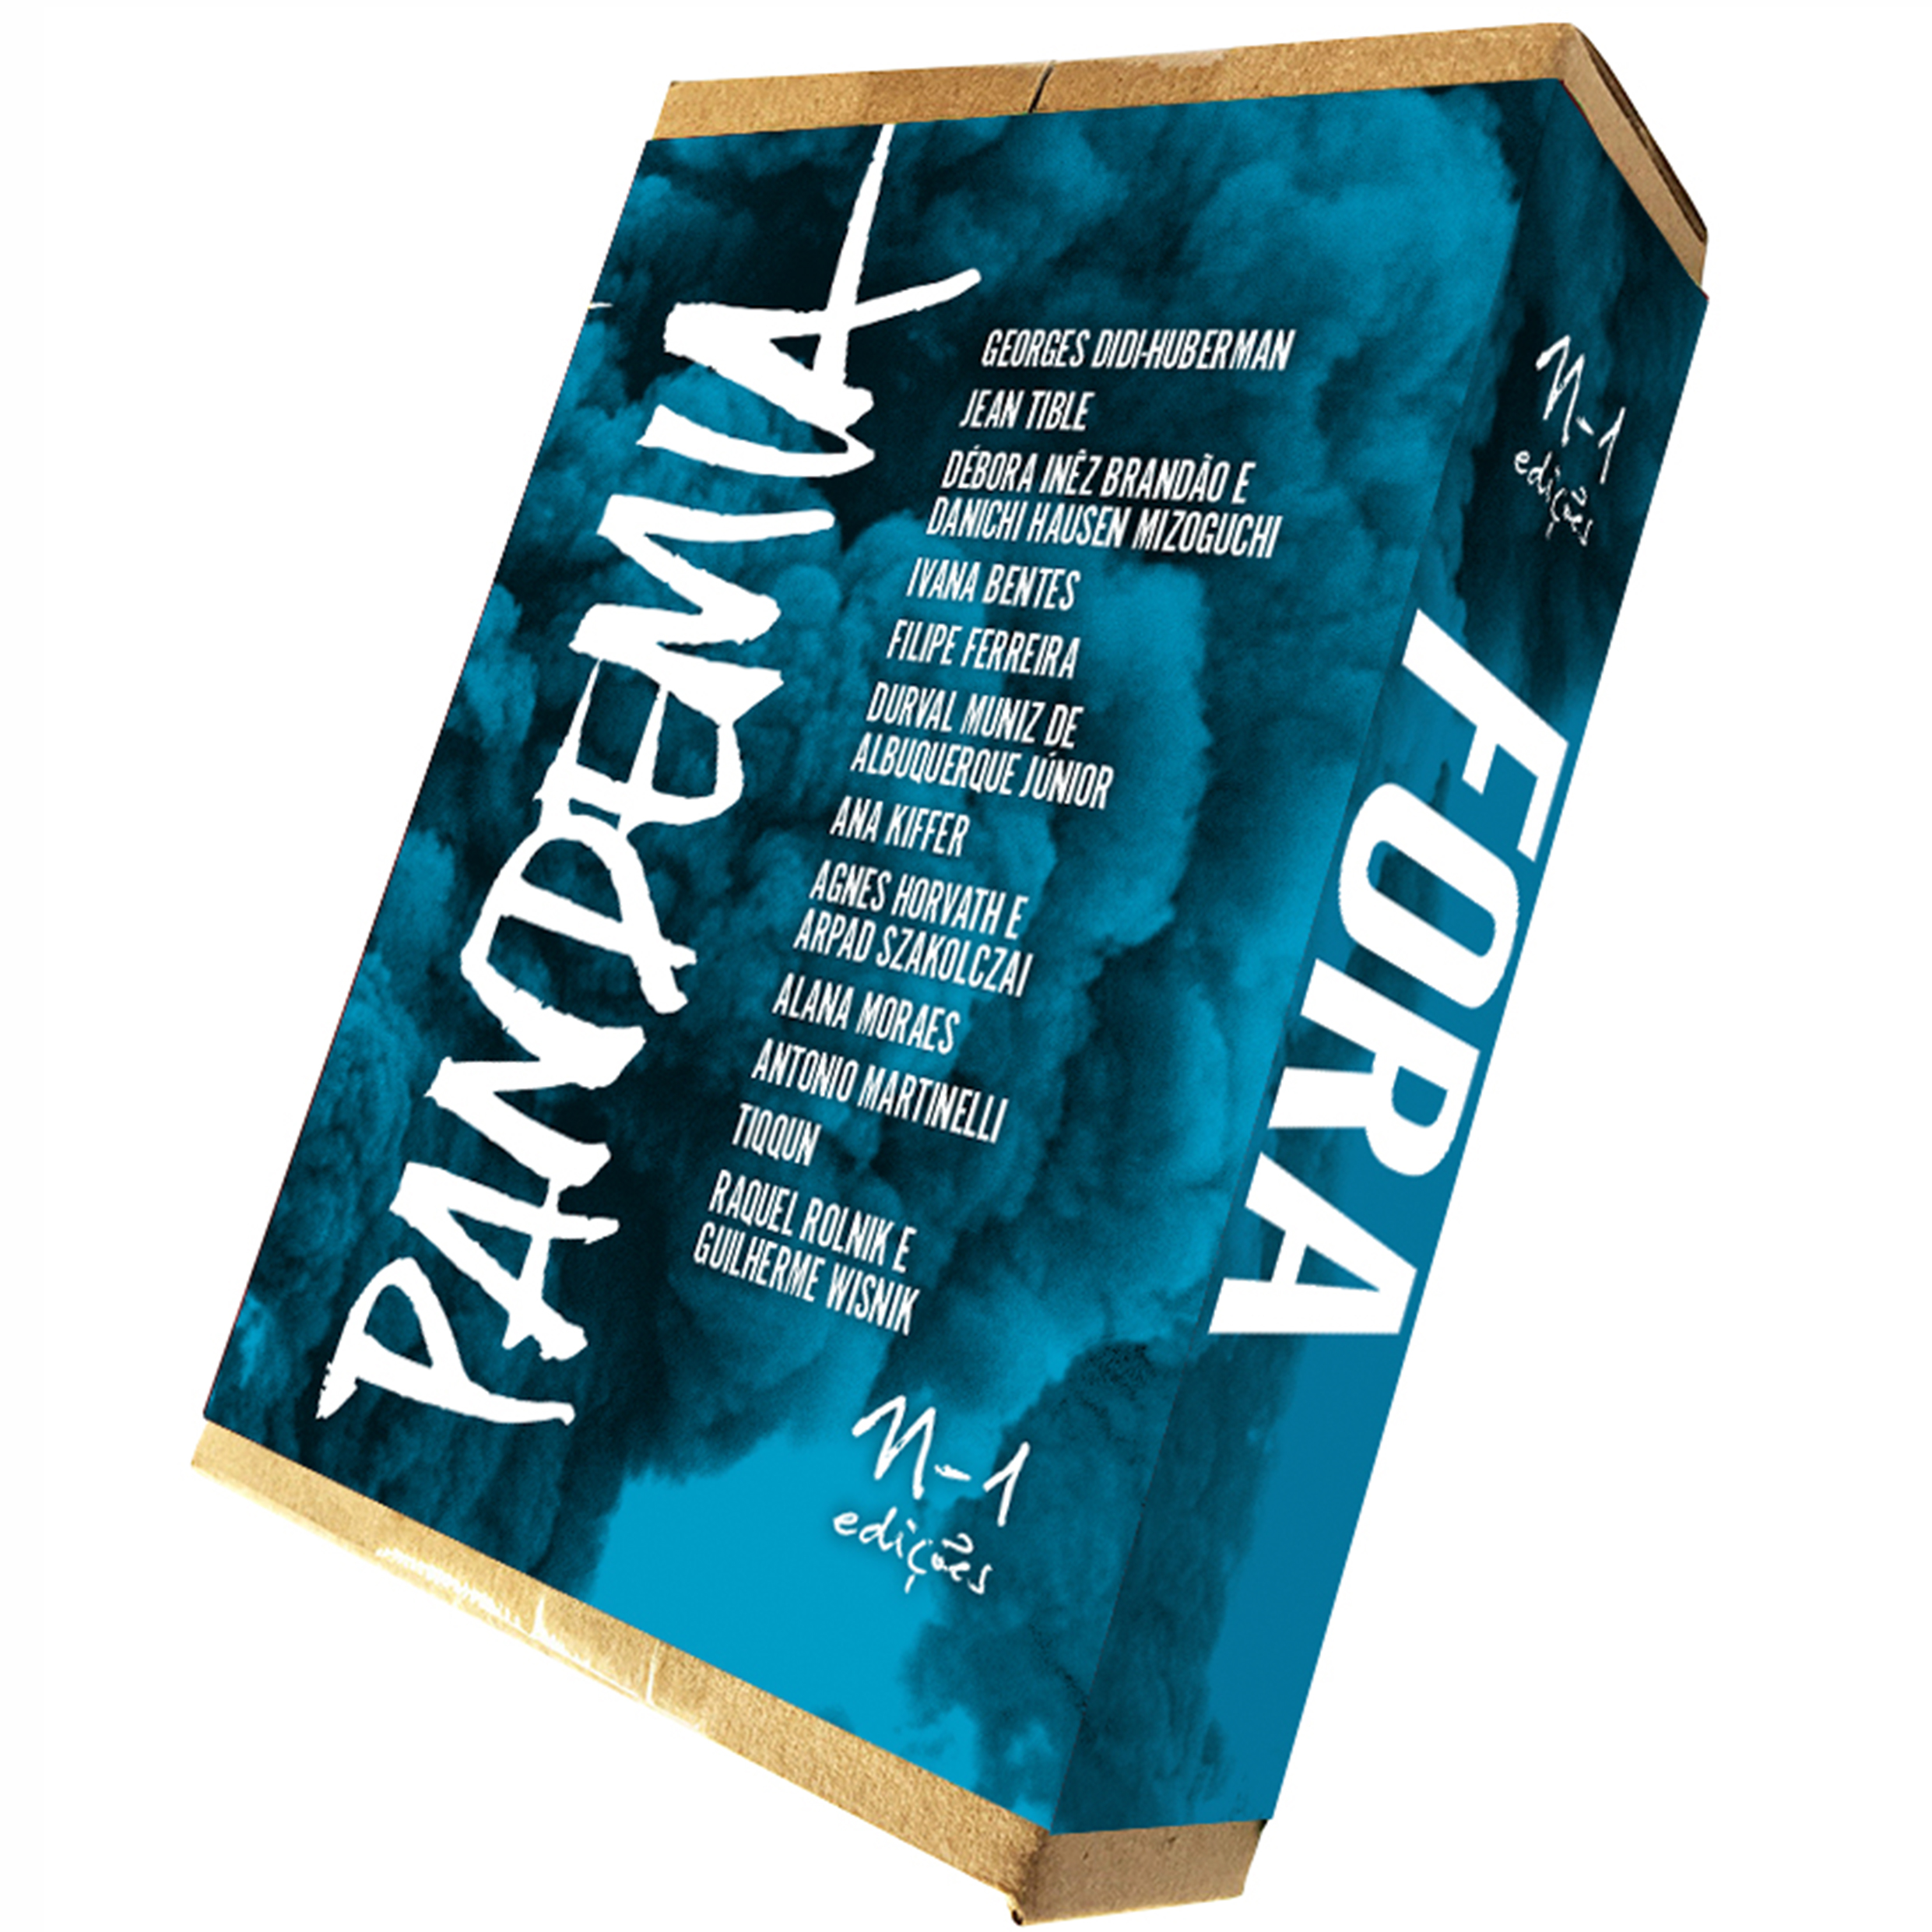
\includegraphics[width=74mm]{./CAPAS/N-1_CAIXA.jpg}
\end{center}

\hspace*{-7cm}\hrulefill\hspace*{-7cm}

\medskip

\noindent{} Caixa \hlc{composta por 12 textos dos seguintes autores}: Georges Didi-Huberman, Débora Inêz Brandão, Danich Hausen Mizoguchi, Durval Muniz de Albuquerque Júnior, Tiqqun, Ivana Bentes, Filipe Ferreira, Ana Kiffer, Agnes Horvath, Arpad Szakolczai, Alana Moraes, Antonio Martinelli, Jean Tible, Raquel Rolnik e Guilherme Wisnik.

\vfill

\hspace*{-.4cm}\begin{minipage}[c]{.5\linewidth}
\small\textbf{
\hspace*{-.1cm}Editora: n-1\\
Título: Caixa Fora\\
Autor: Vários\\
ISBN: 978-65-86941-48-7\\
Páginas: 355\\
Formato: 19x11\,cm\\
Preço: R\$ 85,00\\
}
\end{minipage}

\pagebreak

\begin{center}
\hspace*{-3.6cm}\raisebox{5cm}{\rotatebox[origin=t]{90}{\huge\textbf{Lançamento}}}
\hspace*{3.1cm}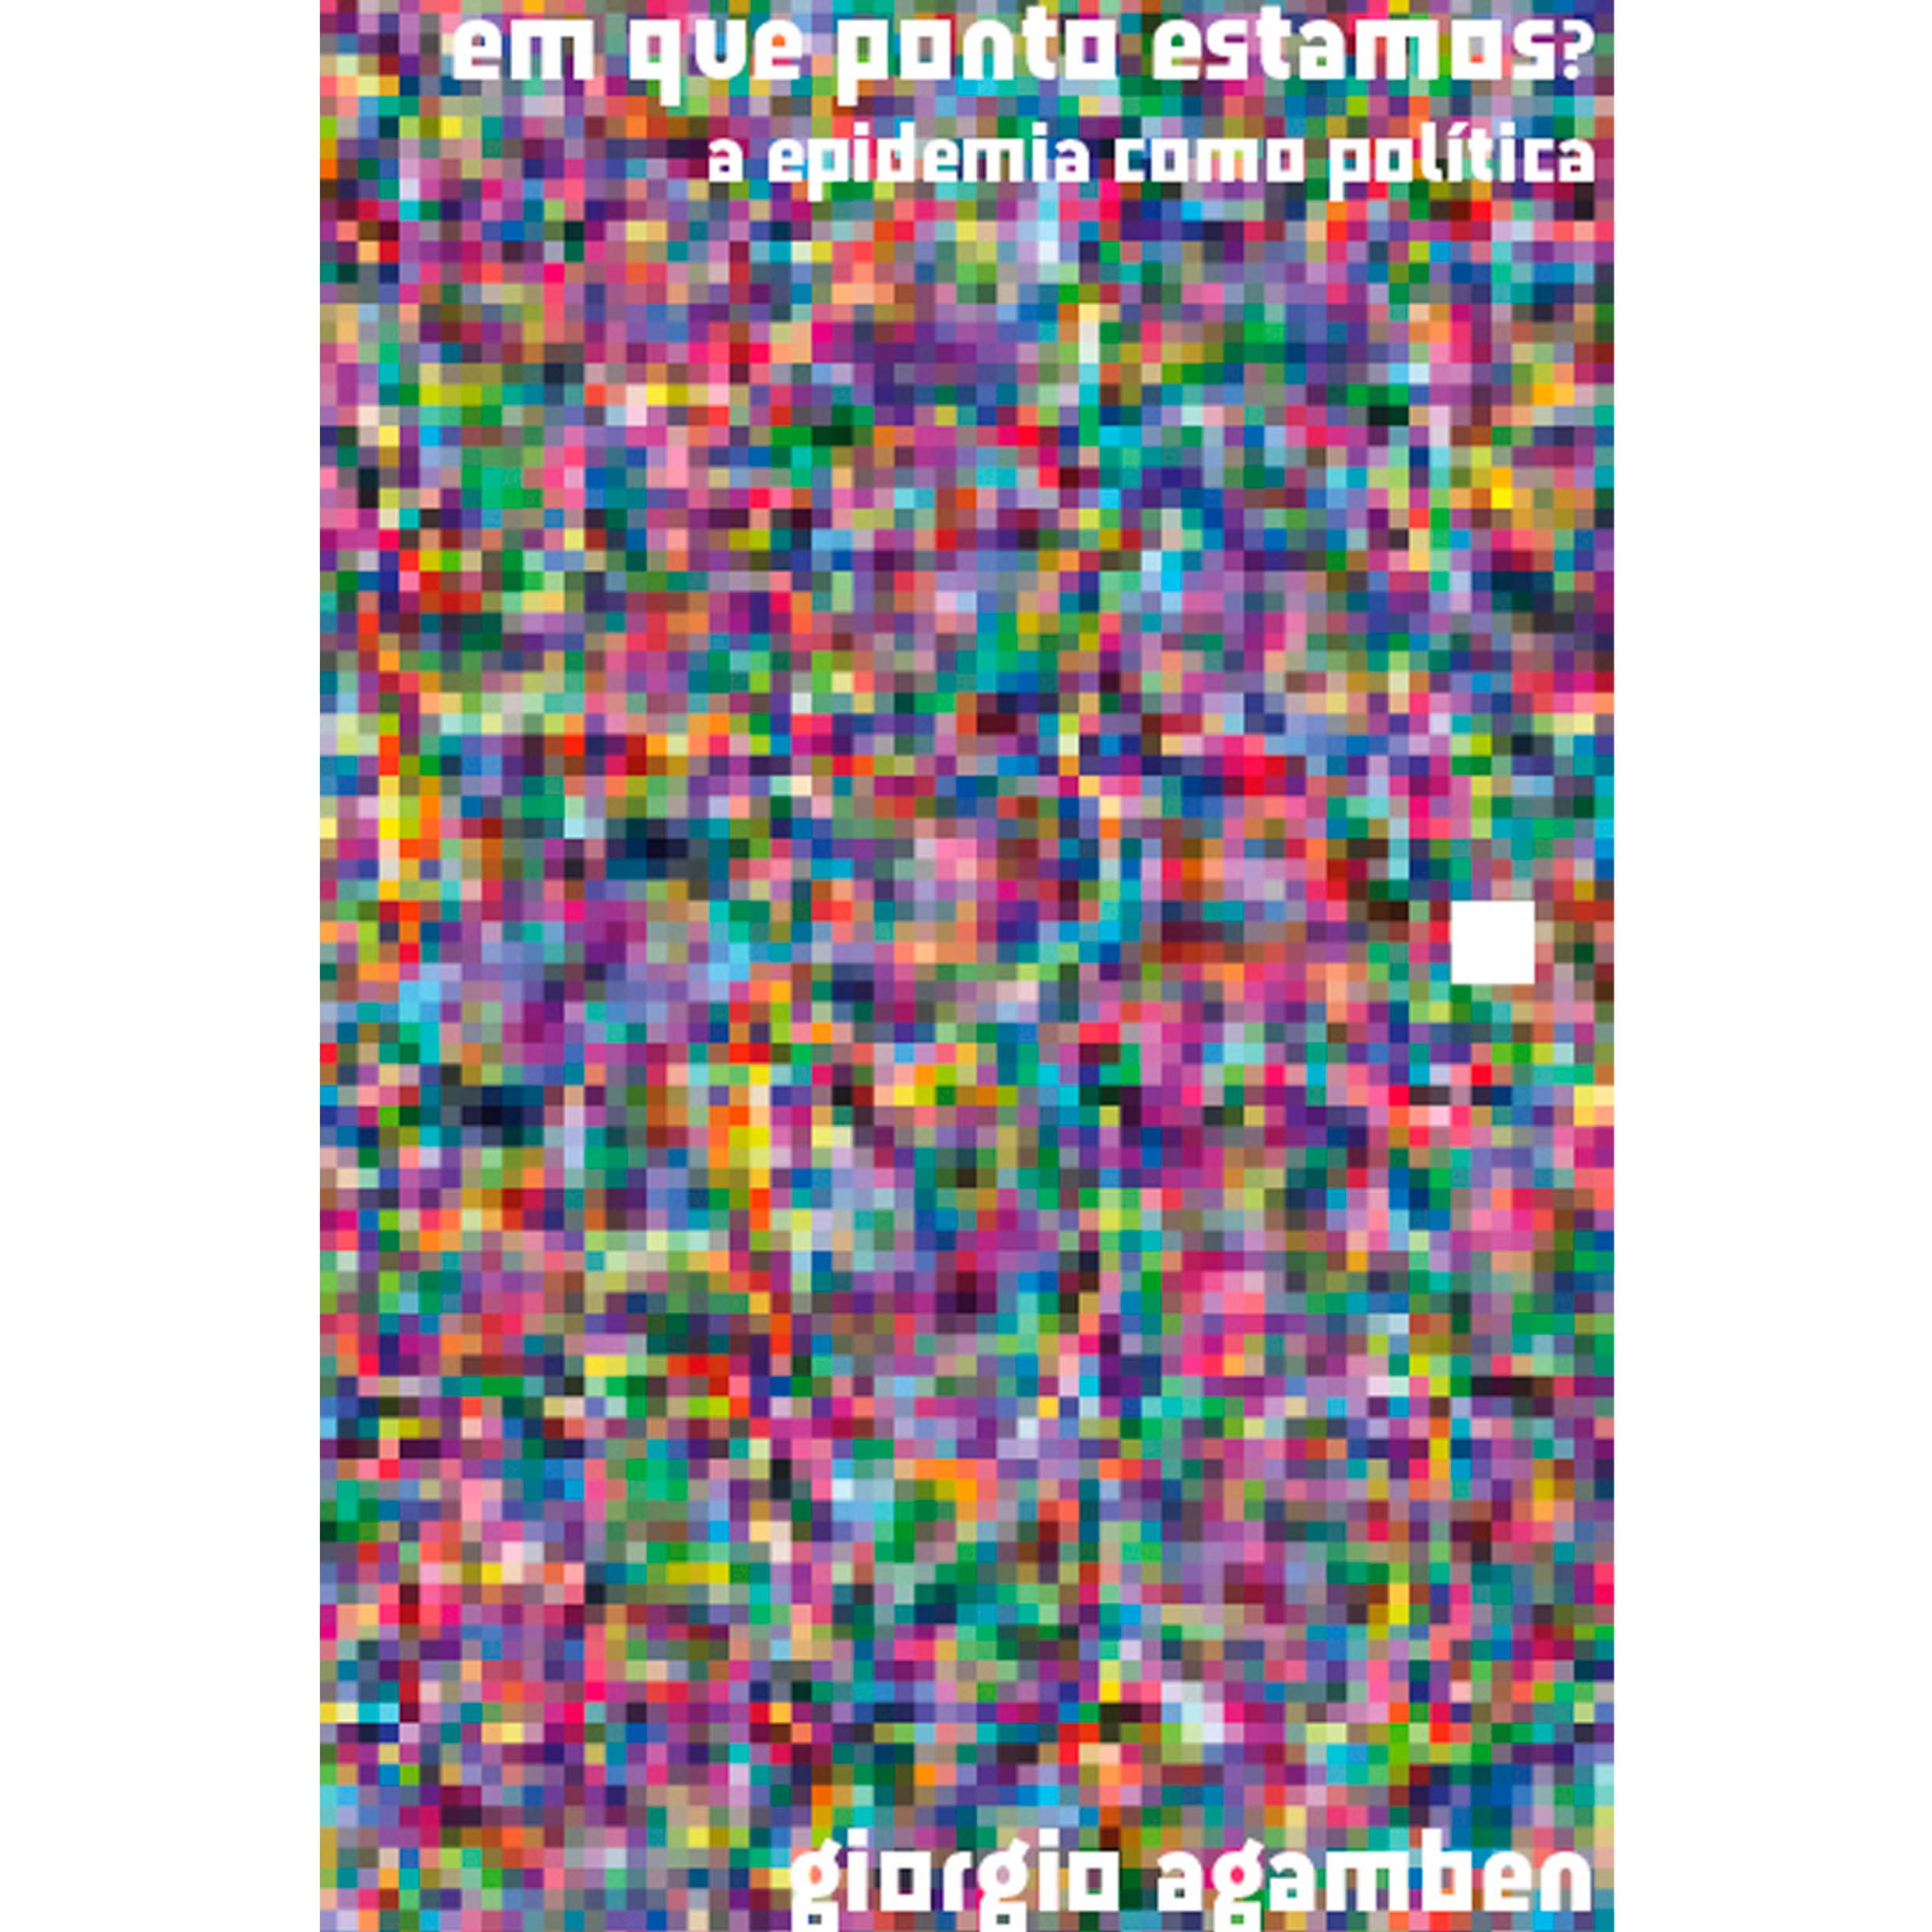
\includegraphics[width=74mm]{./CAPAS/N-1_AGAMBEN.jpg}
\end{center}

\hspace*{-7cm}\hrulefill\hspace*{-7cm}

\medskip

\noindent{}Teremos, em uma palavra, que nos colocar seriamente \hlc{a única pergunta que conta, que não é, como repetem há séculos os falsos filósofos, \textit{de onde viemos} ou \textit{para onde vamos?}, mas, simplesmente, \textit{em que ponto estamos?}.} Esta é a pergunta à qual deveremos tentar responder, do modo que pudermos e onde quer que estejamos, mas, em todo caso, com a nossa vida e não apenas com as palavras.

\vfill

\hspace*{-.4cm}\begin{minipage}[c]{1\linewidth}
\small\textbf{
\hspace*{-.1cm}Editora: n-1\\
Título: Em que ponto estamos?\\
Autor: Giorgio Agamben\\
ISBN: 978-65-86941-55-5\\
Páginas: 128\\
Formato: 21x14\,cm\\
Preço: R\$ 68,00\\
}
\end{minipage}

\pagebreak


\begin{center}
\hspace*{.5cm}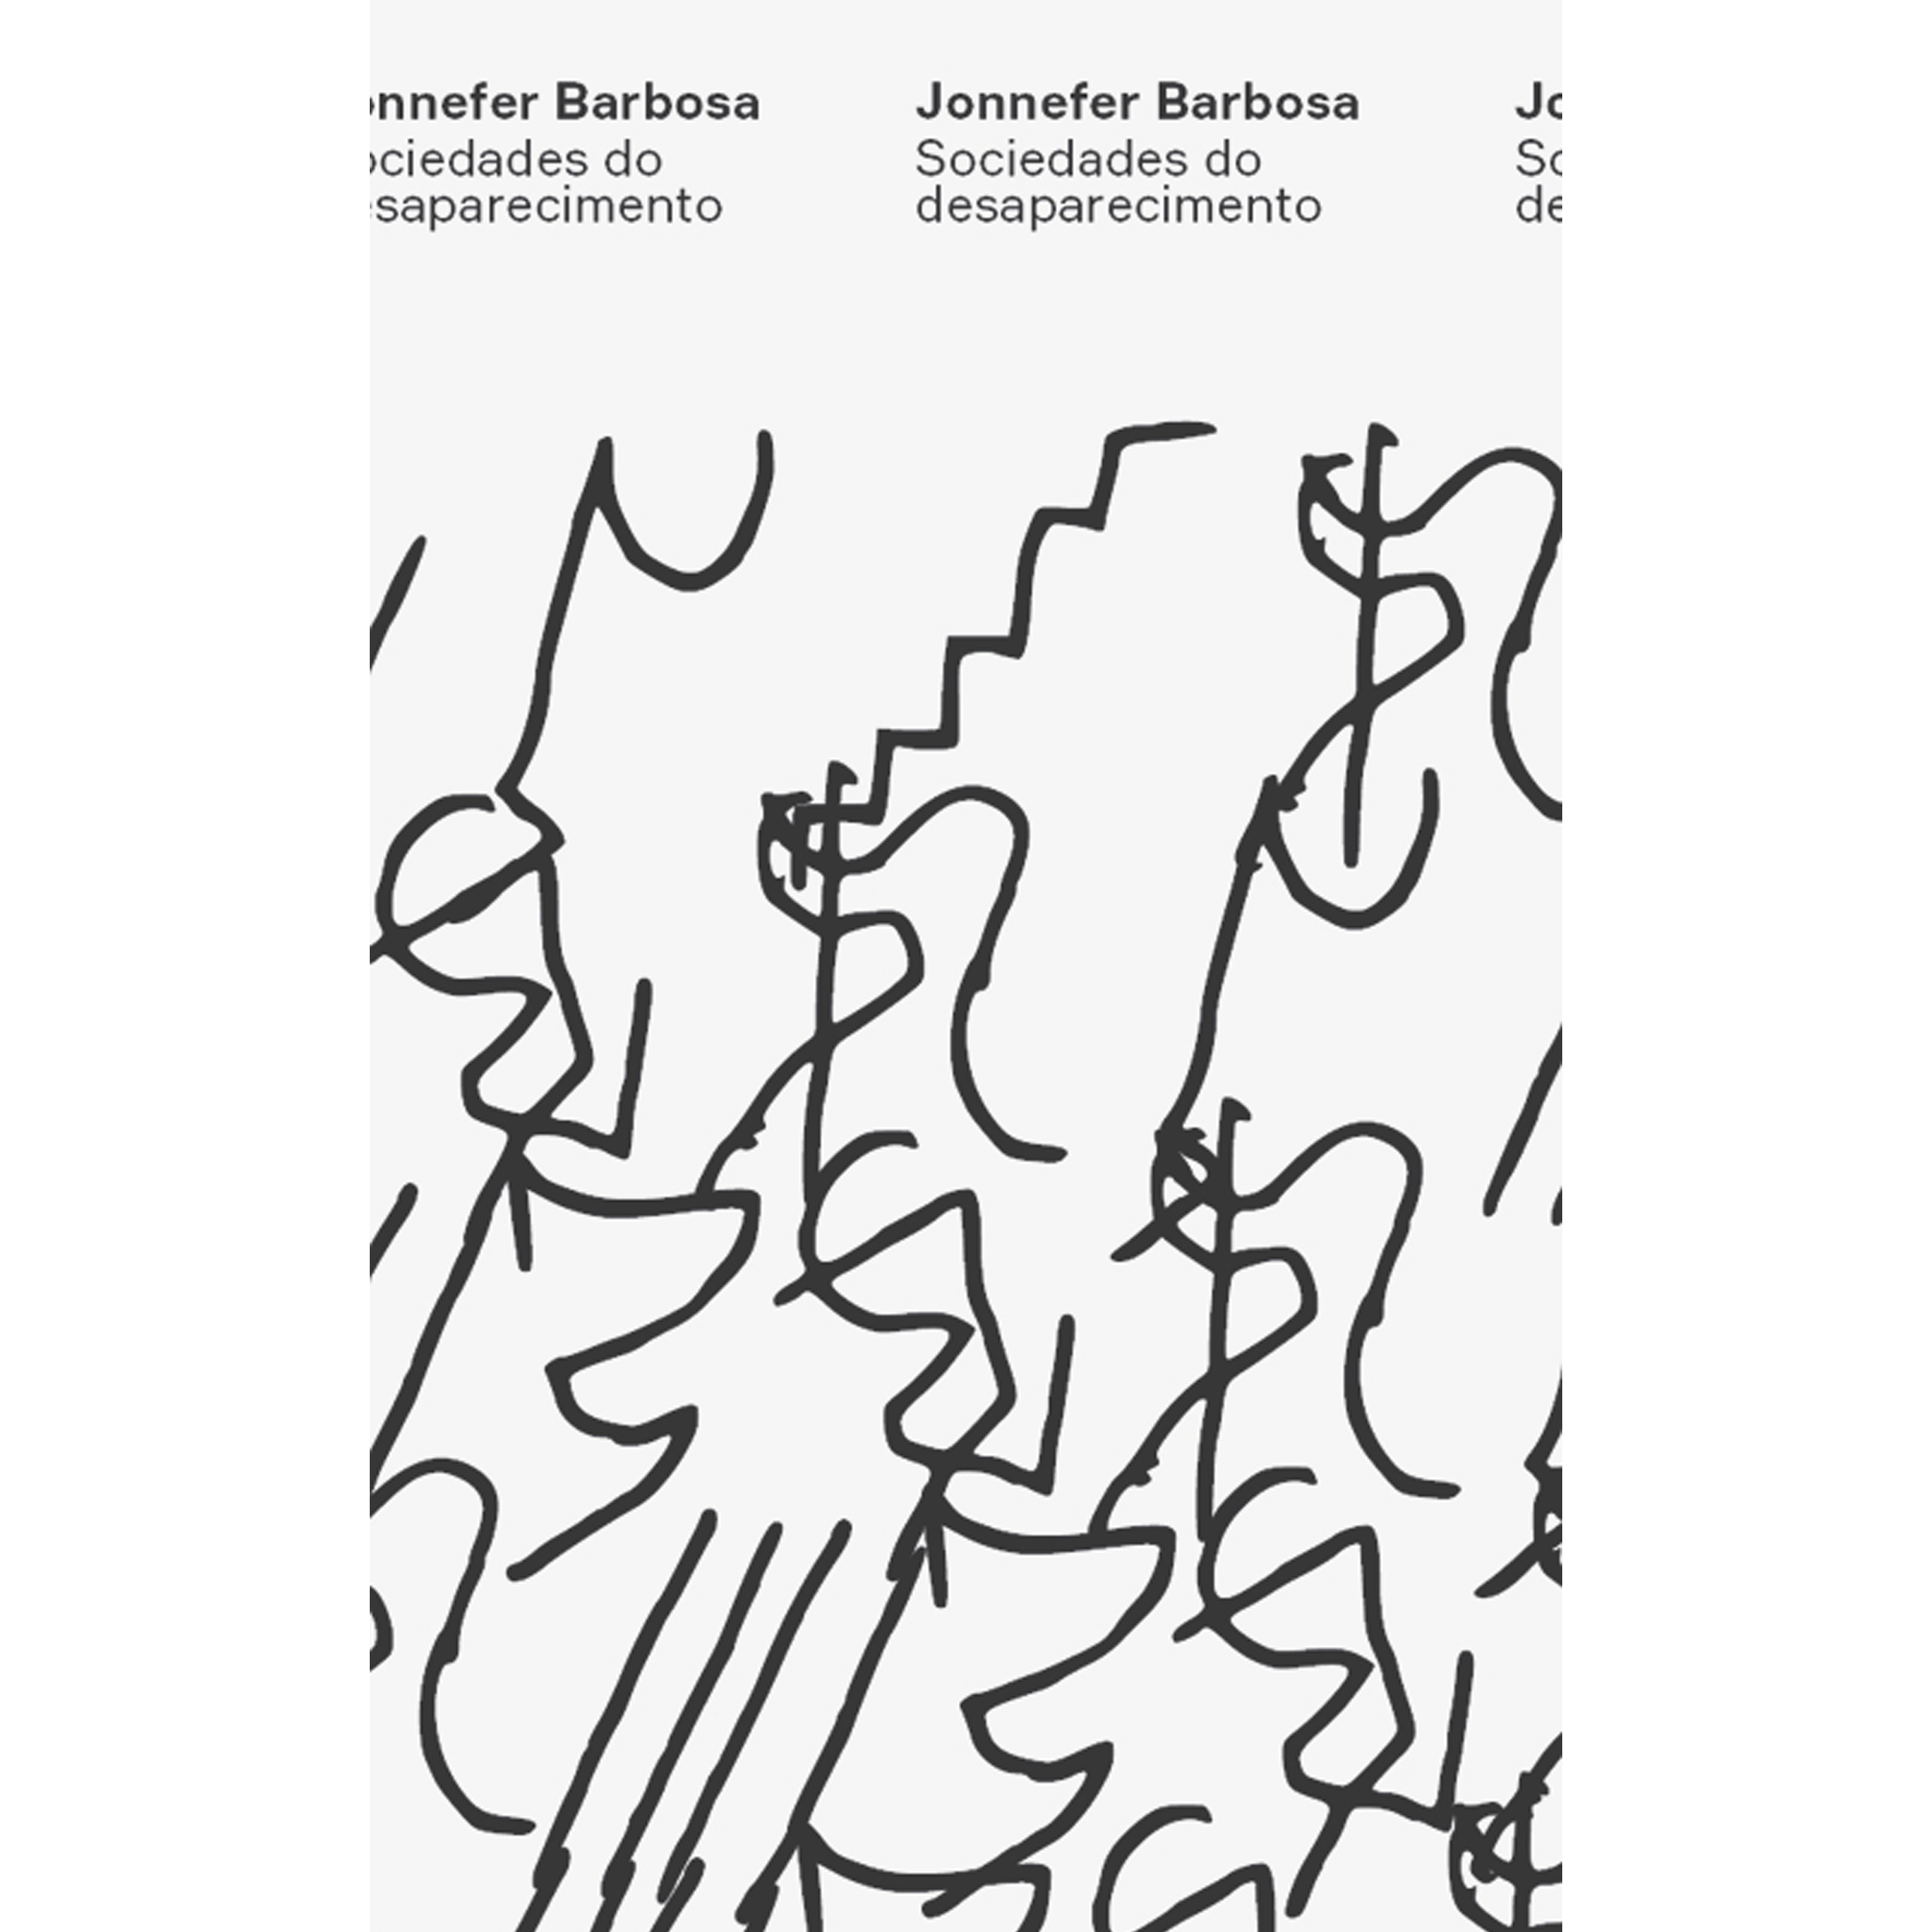
\includegraphics[width=74mm]{./CAPAS/N-1_BARBOSA.jpg}
\end{center}

\hspace*{-7cm}\hrulefill\hspace*{-7cm}

\medskip

\noindent{}O desaparecimento enquanto técnica governamental expõe uma desterritorialização da gestão biopolítica de populações. Tratava-se nesta de governar a impessoalidade da vida biológica. \hlc{A multiplicidade das novas modalidades do poder nas sociedades do desaparecimento expressa-se em diversos e singulares dispositivos, com caracteres e intensidades variáveis.} Do algoritmo criptocibernético à normalização do aniquilamento e da execução sumária como práticas de governo, protagonizadas pelos aparatos policiais ou paraestatais.  Formas de violência gestadas em territórios como a América Latina, que hoje se disseminam como modelo paradigmático e explicativo de uma diagrama governamental mundial.

\vfill

\hspace*{-.4cm}\begin{minipage}[c]{1\linewidth}
\small\textbf{
\hspace*{-.1cm}Editora: n-1\\
Título: Sociedades do desaparecimento\\
Autor: Jonnefer Barbosa\\
ISBN: 978-65-86941-43-2\\
Páginas: 80\\
Formato: 18x11\,cm\\
Preço: R\$ 44,00\\
}
\end{minipage}

\pagebreak

\begin{center}
\hspace*{-3.6cm}\raisebox{5cm}{\rotatebox[origin=t]{90}{\huge\textbf{Lançamento}}}
\hspace*{3.1cm}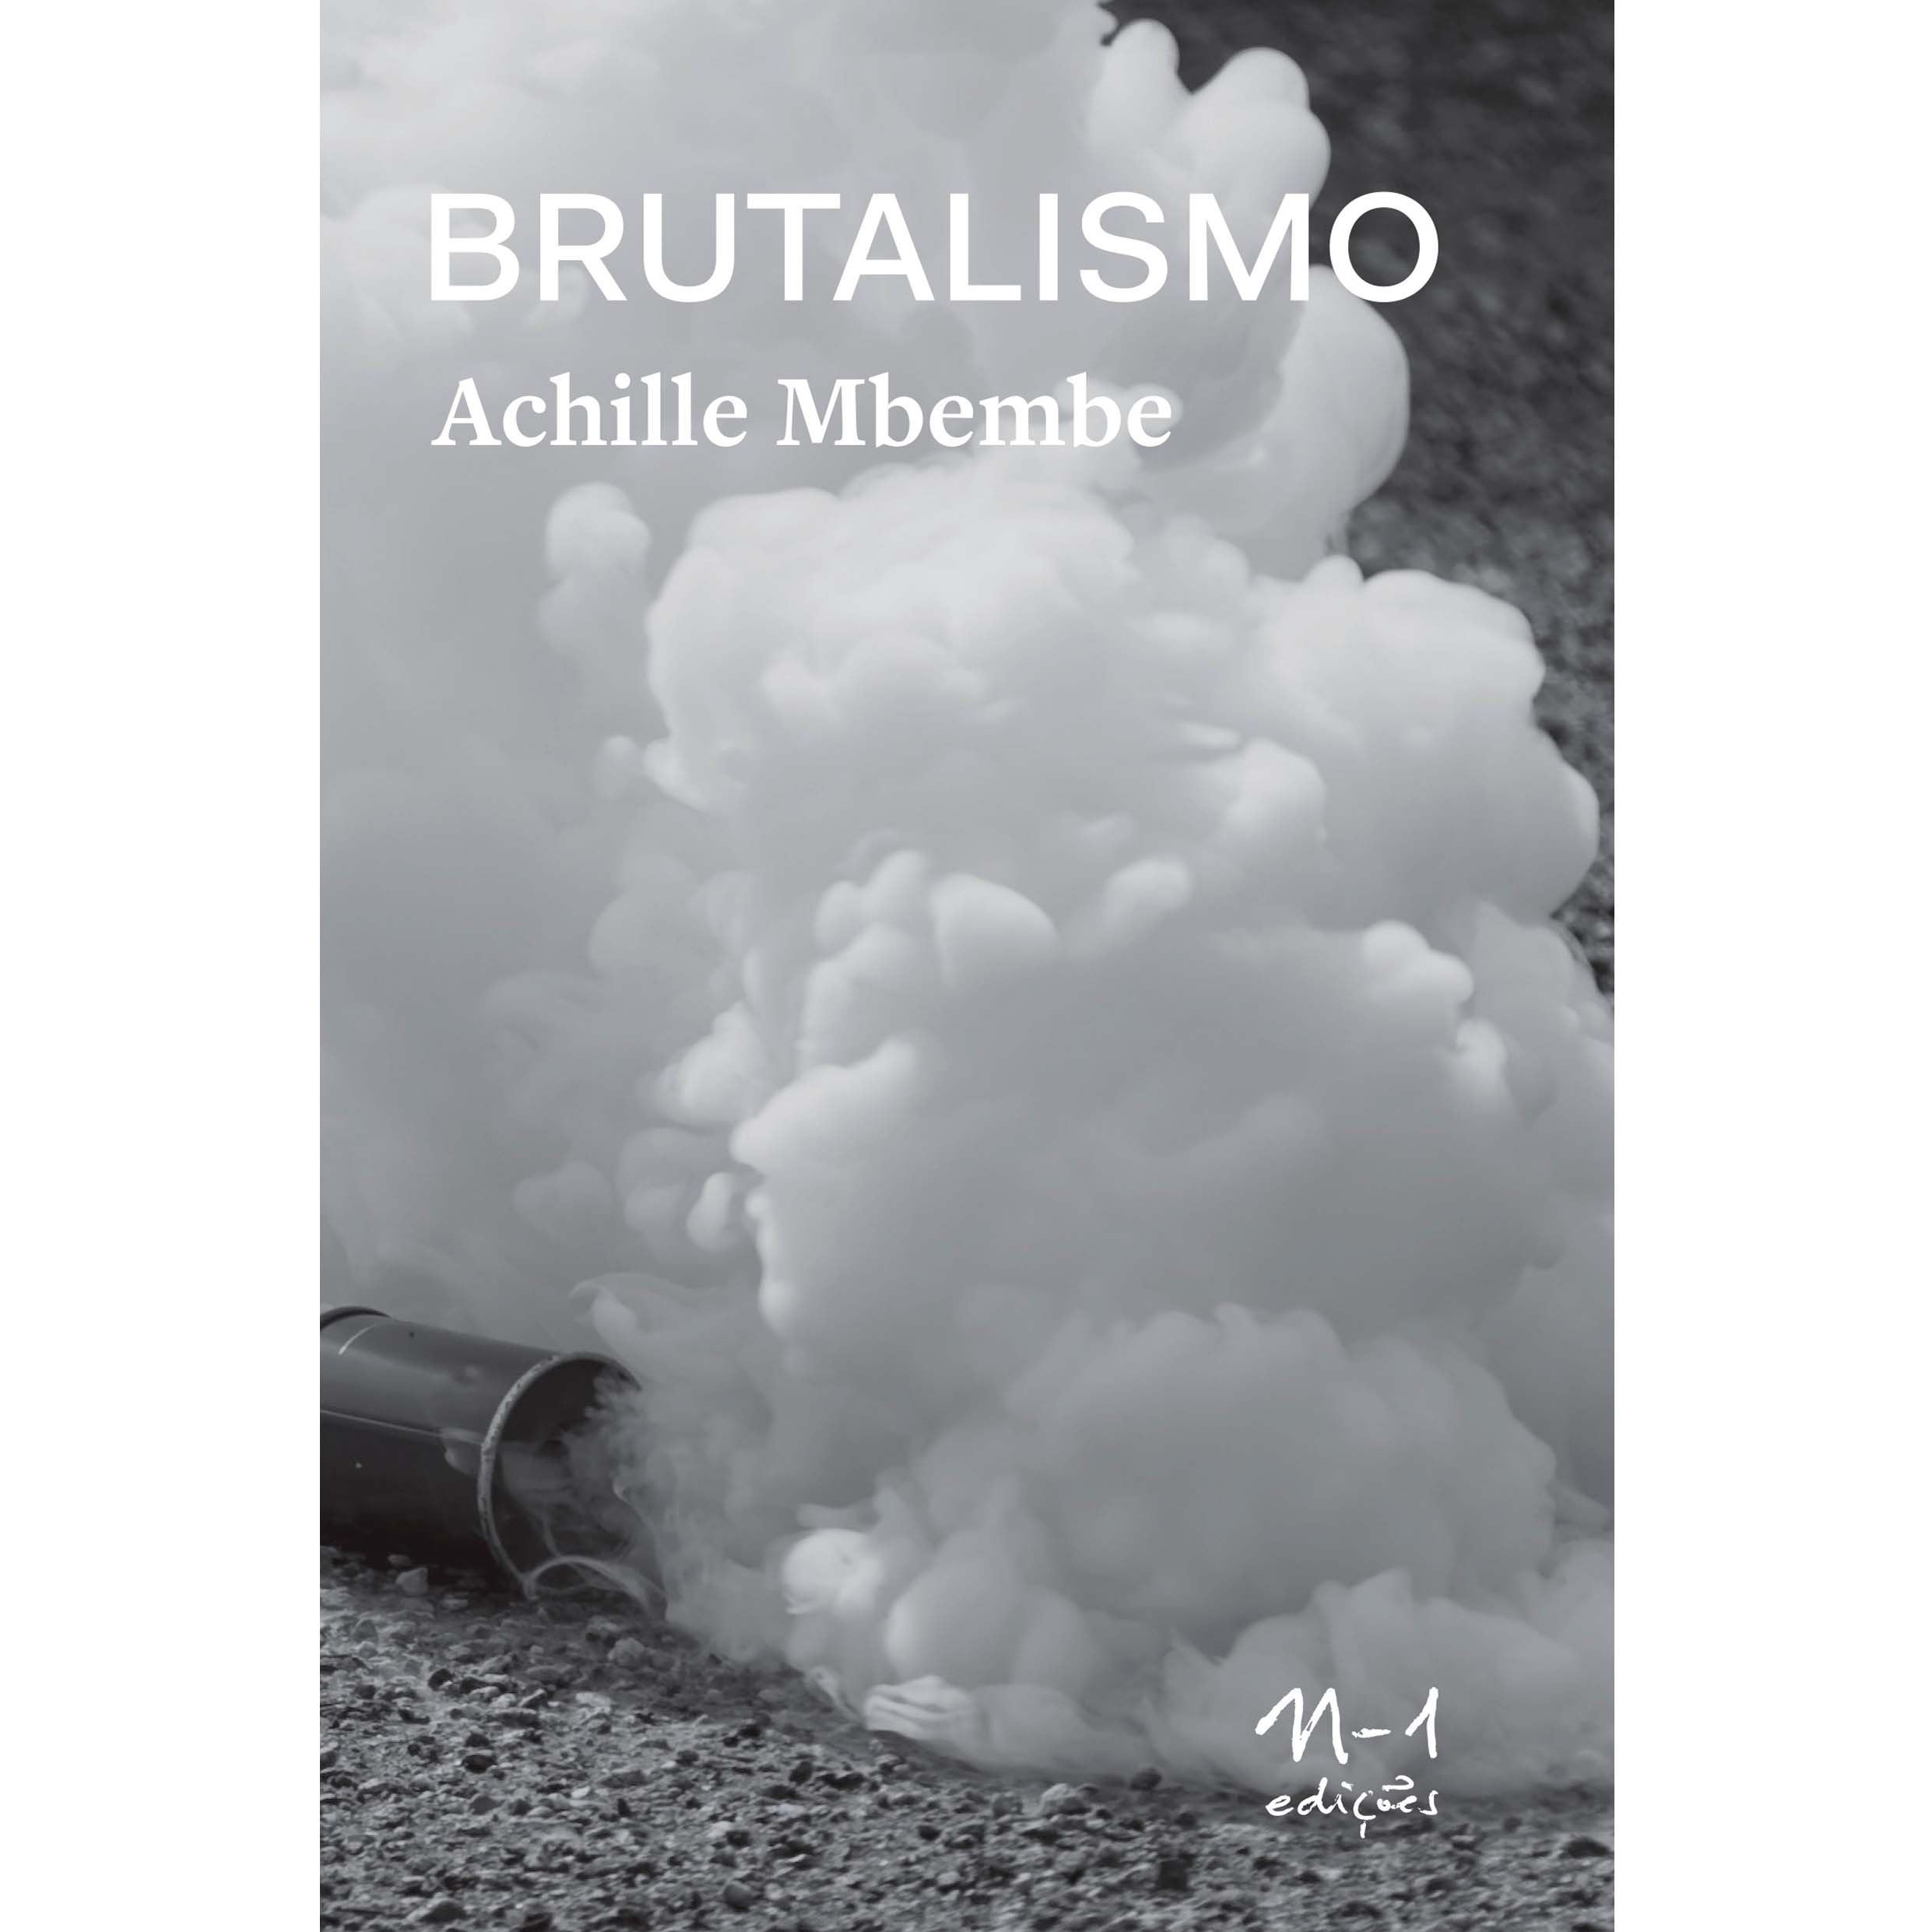
\includegraphics[width=74mm]{./CAPAS/N-1_MBEMBE.jpg}
\end{center}

\hspace*{-7cm}\hrulefill\hspace*{-7cm}

\medskip

\noindent{} Um vasto empreendimento de ocupação territorial, de domínio sobre os corpos e os imaginários, de desmontagem, dissociação e demolição está em curso. Ele conduz, praticamente em toda parte, a \textit{estados de emergência} ou \textit{exceção}, que logo se estendem a permanentes. \hlc{As modalidades contemporâneas de demolição se cristalizam, enquanto as clássicas dicotomias forma/\,matéria, matéria/\,material, material/\,imaterial, natural/\,artificial e fim/\,meio são profundamente questionadas.} A lógica das oposições foi substituída pela das permutações, convergências e conversões múltiplas. Não há mais nenhuma matéria intrinsecamente disponível e dócil. Ela existe apenas coconstituída a partir de uma heterogeneidade de matrizes e conexões.

\vfill

\hspace*{-.4cm}\begin{minipage}[c]{1\linewidth}
\small\textbf{
\hspace*{-.1cm}Editora: n-1\\
Título: Brutalismo\\
Autor: Achille Mbembe\\
ISBN: 978-65-86941-62-3\\
Páginas: 256\\
Formato: 21x14\,cm\\
Preço: R\$ 90,00\\
}
\end{minipage}

\pagebreak

\begin{center}
\hspace*{.5cm}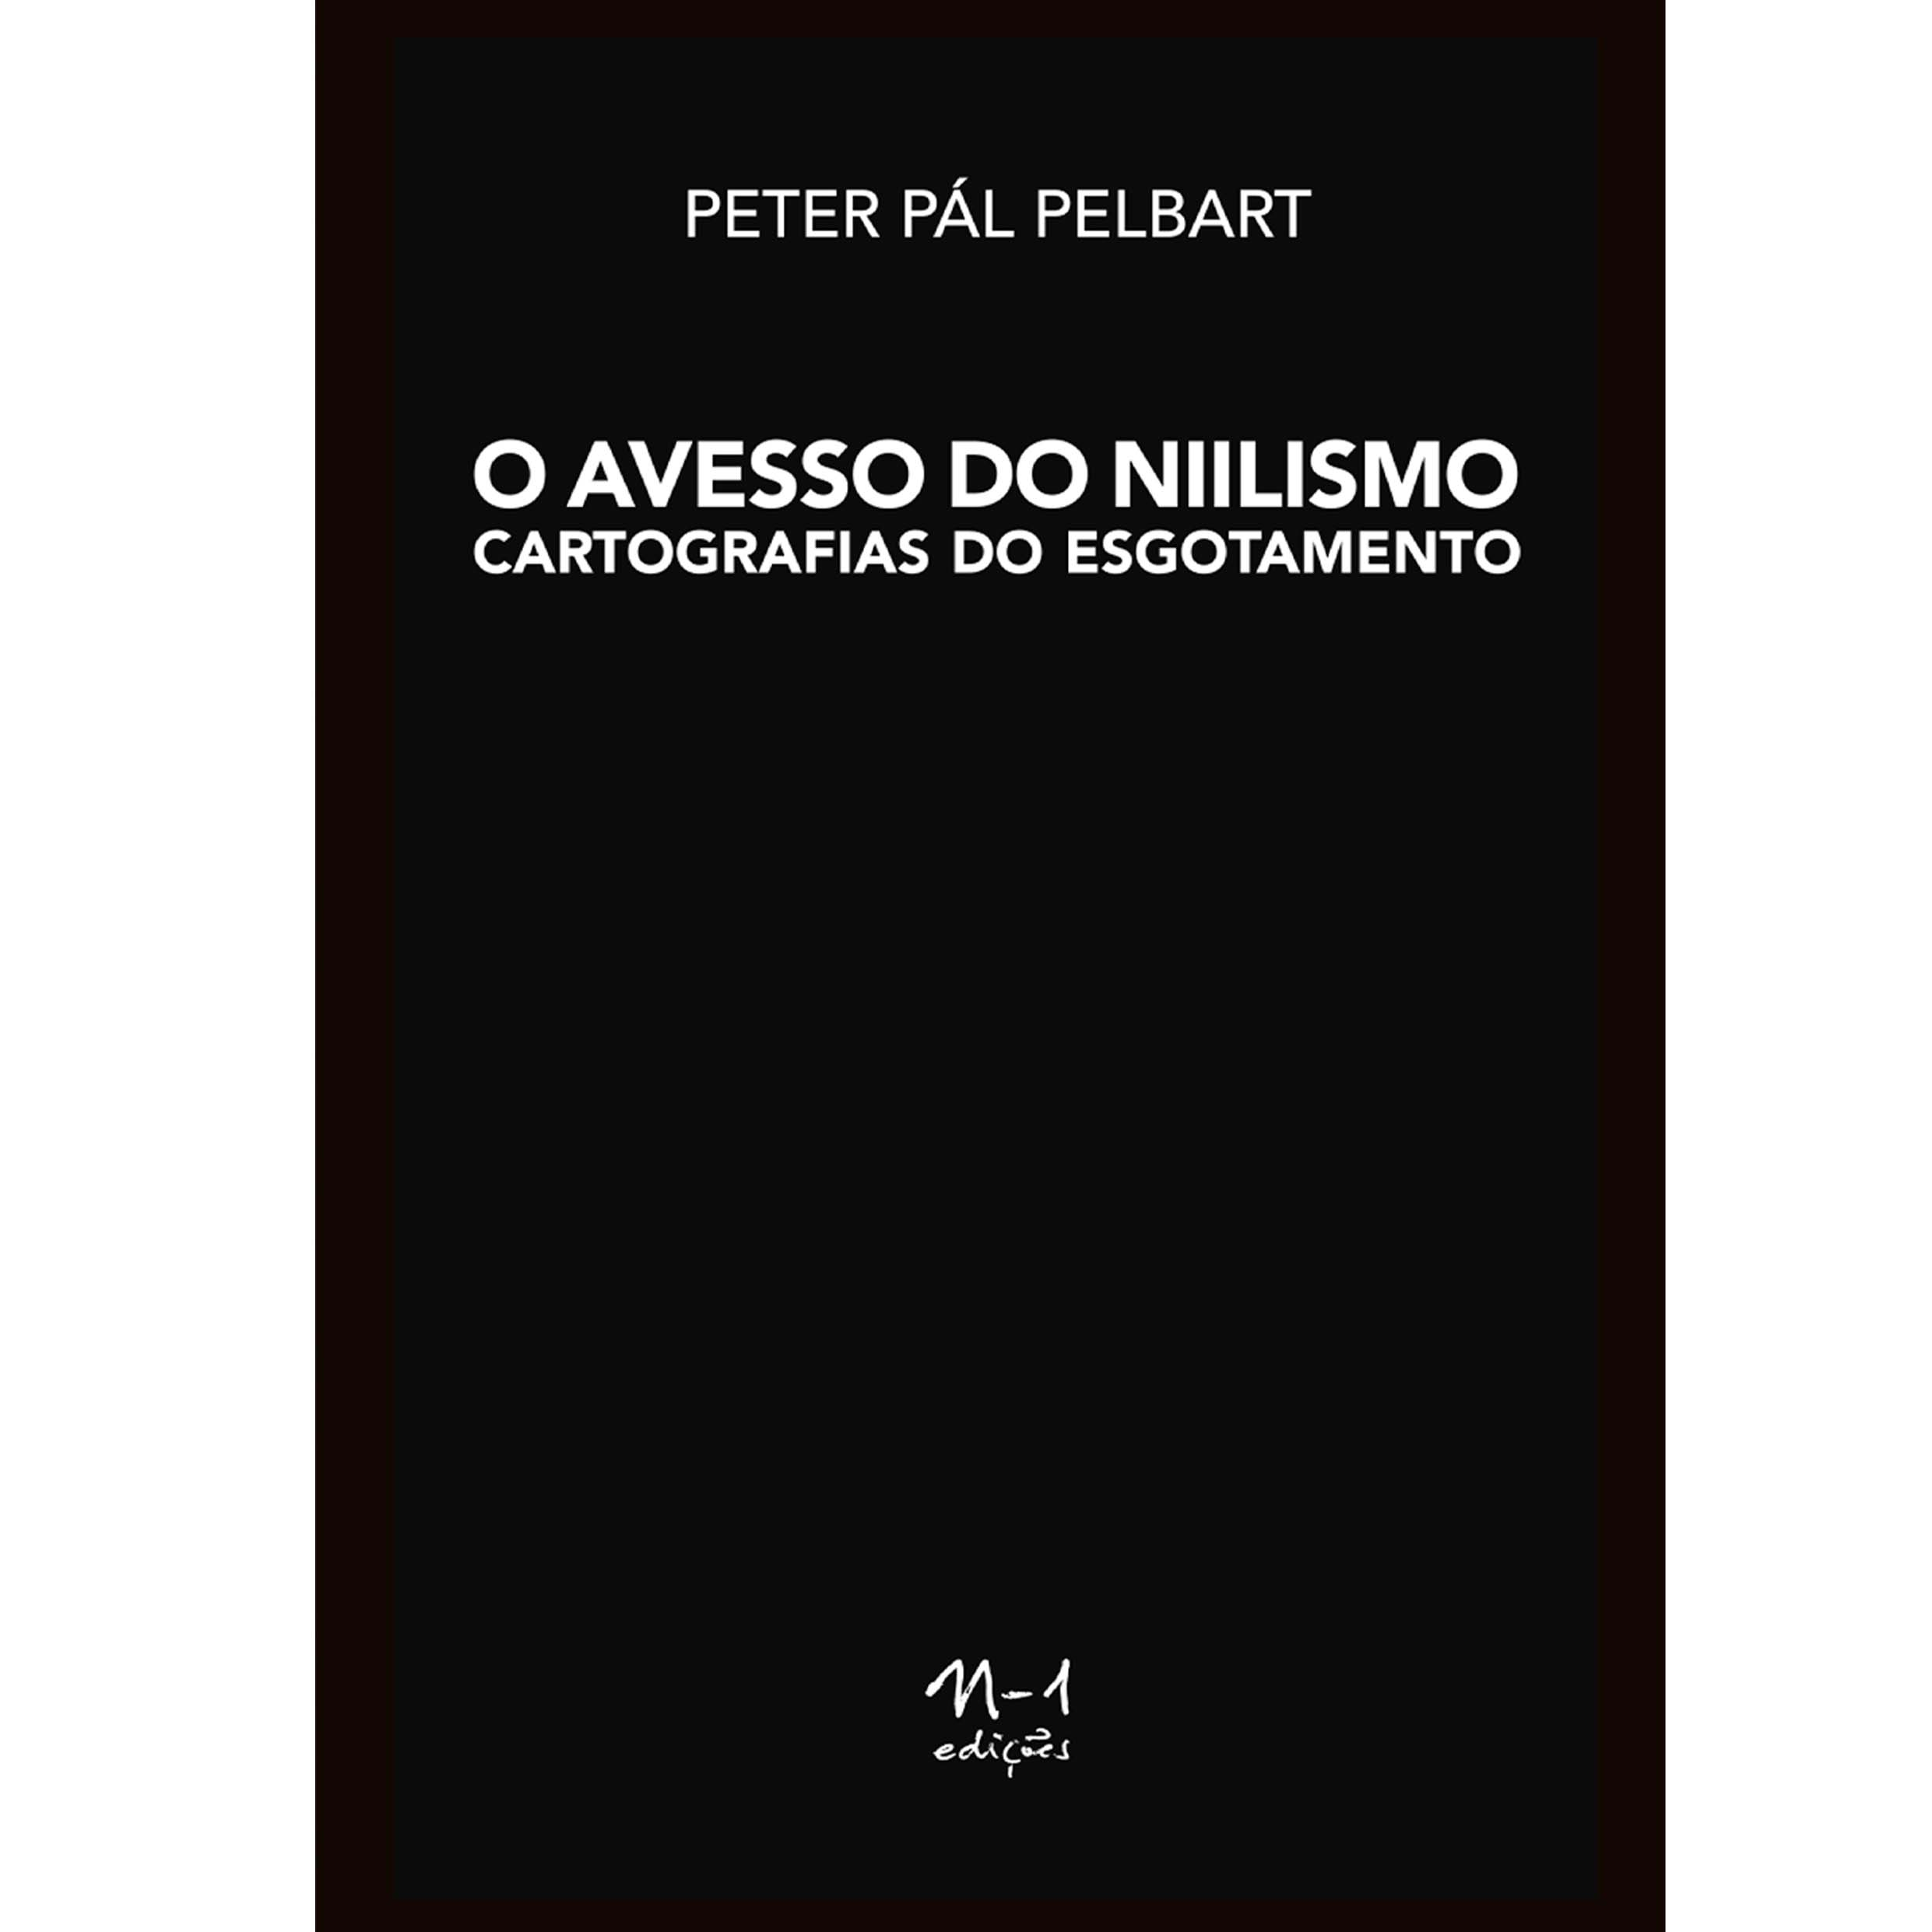
\includegraphics[width=74mm]{./CAPAS/N-1_PELBART.jpg}
\end{center}

\hspace*{-7cm}\hrulefill\hspace*{-7cm}

\medskip

\noindent{}Afinal, do que é que estamos tão esgotados? Inspirado em um vasto leque de autores --- de Musil a Blanchot, Deleuze, Agamben, Jünger, Sloterdijk ---, mas também apoiado em experiências"-limite de Deligny ou trabalhos esquizo"-cênicos, \textit{O avesso do niilismo} apresenta indícios de um deslocamento em curso. De quem? Do quê? Em qual direção? Não sabemos ao certo. 

É uma cartografia coletiva, inacabada, movente, que indica pontos de estrangulamento através dos quais, nos \textit{avessos do niilismo} biopolítico, se liberam outras energias, visões, noções. \hlc{Não se trata de saber \textit{quem fala}, nem \textit{de qual lugar se fala}, mas, como o sugeriu Guattari, \textit{o que fala através de nós}}: uma cartografia do esgotamento, espécie de sintomatologia molecular de Beckett.

\vfill

\hspace*{-.4cm}\begin{minipage}[c]{1\linewidth}
\small\textbf{
\hspace*{-.1cm}Editora: n-1\\
Título: O avesso do niilismo\\
Autor: Peter Pál Pelbart\\
ISBN: 978-65-86941-64-7\\
Páginas: 448\\
Formato: 21x14\,cm\\
Preço: R\$ 68,00\\
}
\end{minipage}

\pagebreak

\begin{center}
\hspace*{-3.6cm}\raisebox{5cm}{\rotatebox[origin=t]{90}{\huge\textbf{Lançamento}}}
\hspace*{3.1cm}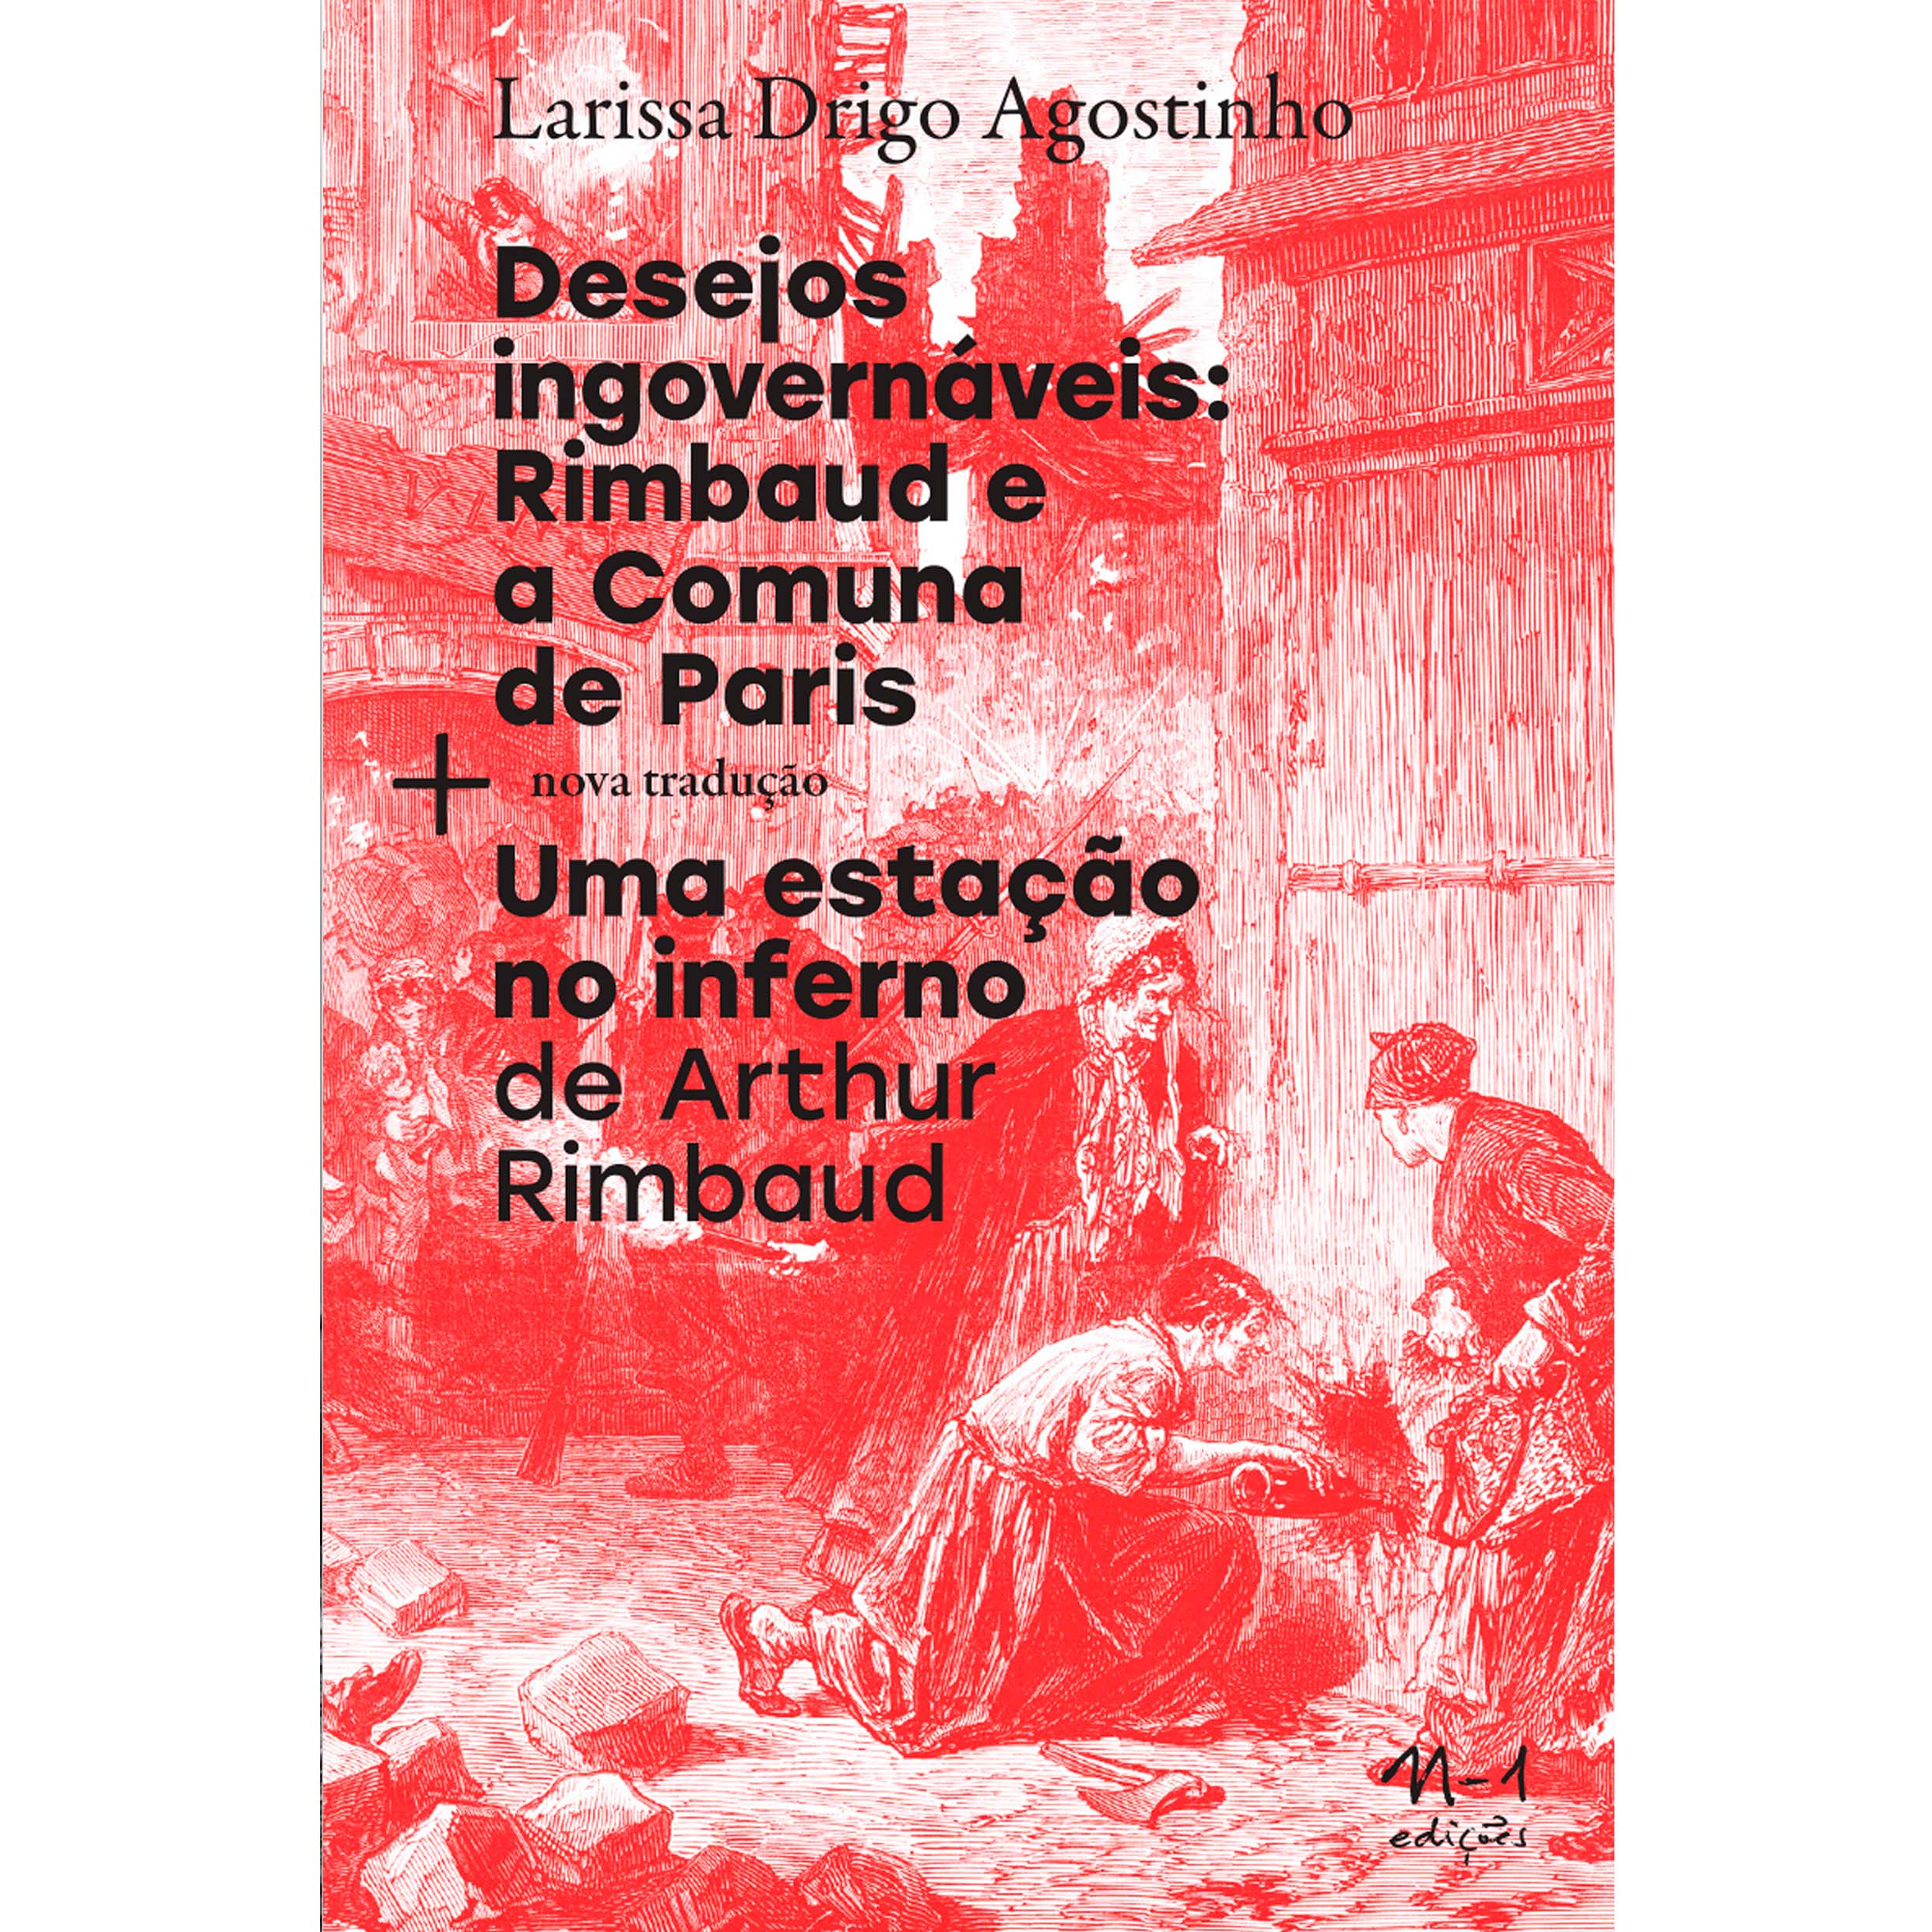
\includegraphics[width=74mm]{./CAPAS/N-1_RIMBAUD.jpg}
\end{center}

\hspace*{-7cm}\hrulefill\hspace*{-7cm}

\medskip

\noindent{}Visões poéticas, assim como as verdadeiras transformações políticas, são resultado de um lento e racionado esforço quase monstruoso que vem, ao mesmo tempo, do corpo e da imaginação. Como as estações, as visões e as revoluções vão e vêm.

\hlc{Não estamos, portanto, diante de um poema descritivo, mas de um poema crítico. Uma crítica da história da França que, às vezes, extravasa e pretende abarcar todo o Ocidente.} Rimbaud não descreve, ele delira as raças e os continentes contra a história demasiado real de uma raça de cérebro estreito que tirava o coro de bestas ferozes, pregava o batismo e fazia os outros trabalharem. Uma raça imperialista de colonizadores, de homens que se tomam por fortes, mas são brutais; uma raça branca que faz o narrador declarar pertencer a outra raça, inferior para toda a eternidade.
\vfill

\hspace*{-.4cm}\begin{minipage}[c]{1\linewidth}
\small\textbf{
\hspace*{-.1cm}Editora: n-1\\
Título: Desejos ingovernáveis: Rimbaud e a\\comuna de Paris + Uma estação no inferno\\
Autor: Larissa Drigo Agostinho e\\Arthur Rimbaud\\
ISBN: 978-65-86941-52-4\\
Páginas: 196\\
Formato: 19x11\,cm\\
Preço: R\$ 68,00\\
}
\end{minipage}

\pagebreak

\begin{center}
\hspace*{.5cm}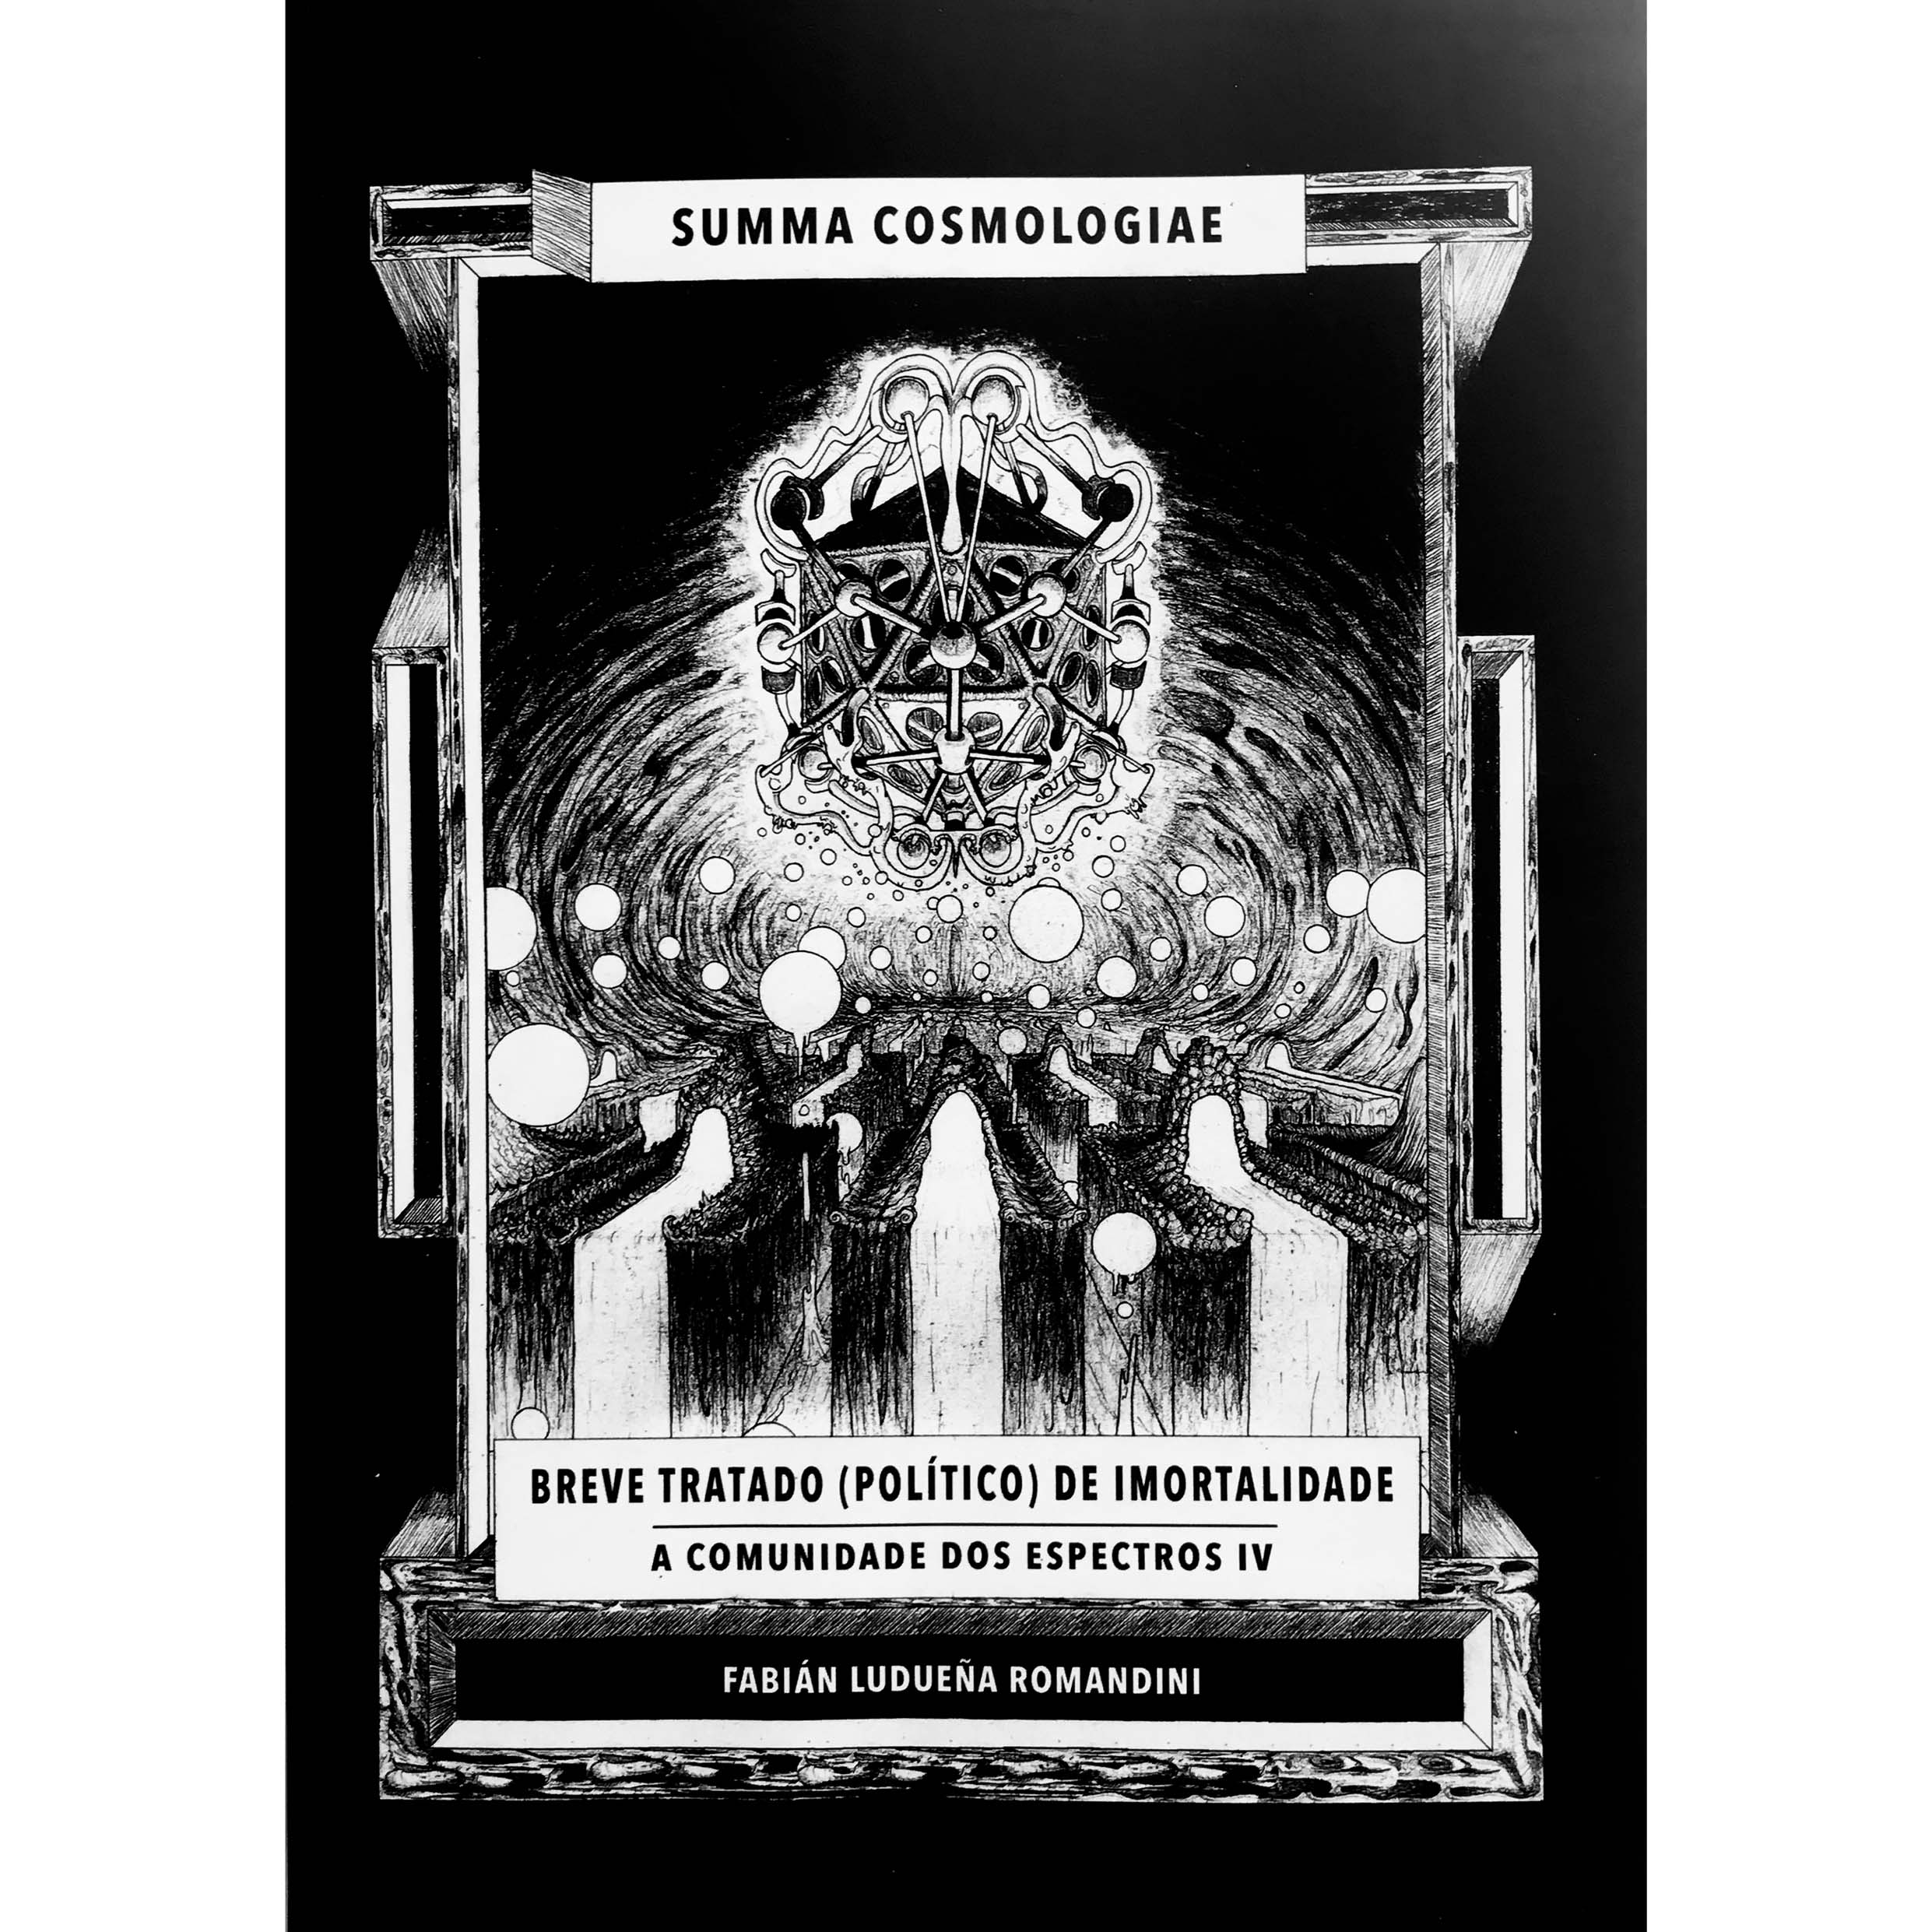
\includegraphics[width=74mm]{./CAPAS/N-1_TRATADO.jpg}
\end{center}

\hspace*{-7cm}\hrulefill\hspace*{-7cm}

\medskip

\noindent{}A filosofia é assim redirecionada para algumas das suas questões cardeais, para as quais procura delinear respostas de um novo tipo: \hlc{em que condições é a cosmologia o conhecimento que pode explicar problemas tão cruciais como a imortalidade ou a diferença sexual?}
Em que sentido se pode falar, filosoficamente, de um \textit{multiverso} numa época em que, como Friedrich Hölderlin já havia salientado, a ciência parece incapaz de satisfazer as exigências dos espíritos criativos? Os postulados teóricos são acompanhados por uma incursão nos meandros da filosofia da história de nosso \textit{éon}, caracterizado pela ascensão dos pós-humanos depois dos últimos dias da humanidade.
\vfill

\hspace*{-.4cm}\begin{minipage}[c]{1\linewidth}
\small\textbf{
\hspace*{-.1cm}Editora: n-1\\
Título: Summa Cosmologiae: Breve\\tratado (político) de imortalidade\\
Autor: Fabián Ludueña Romandini\\
ISBN: 978-65-86941-49-4\\
Páginas: 192\\
Formato: 23x16\,cm\\
Preço: R\$ 62,00\\
}
\end{minipage}

\pagebreak

\vspace*{1.5cm}

\noindent{}{\nohyphens{\LARGE{Arquitetura é uma forma de política}}}

\bigskip

\hfill{}\scalebox{.8}{ACHILLE MBEMBE}

\bigskip
\bigskip
\bigskip

\begin{multicols}{2}
\noindent{}Tomo o conceito de brutalismo de empréstimo ao pensamento
arquitetônico.\footnote{A respeito do movimento brutalista, ler
  especialmente Reyner Banham, \textit{The New Brutalism: Ethic or
  Aesthetic?} London: Architectural Press, 1966. Ver também Alexander
  Clement, \textit{Brutalism: Post"-War British Architecture.} Ramsbury:
  Crowood Press, 2011. No que se refere ao resgate do conceito no campo
  da música e em particular na música eletroacústica, ver Mo H. Zareei,
  Dugal McKinnon, Dale A. Carnegie \& Ajay Kapur, ``Sound"-based
  Brutalism: An Emergent Aesthetic'', \textit{Style and Genre in
  Electroacoustic Music} 21 (Special Issue 1), 2006: 51-60.} Em minha
mente, porém, trata"-se de uma categoria eminentemente política. Como
poderia ser de outra forma, se existe uma dimensão da própria
arquitetura que é, desde o início, política -- a política de materiais
que, inertes ou não, são por vezes considerados indestrutíveis? Por
outro lado, o que é o político senão uma apreensão de elementos de toda
ordem aos quais se tenta dar forma, se necessário pela força, um
exercício de torção e remodelação por excelência?

Além disso, a arquitetura é uma forma de política na medida em que
inevitavelmente desencadeia uma tensão -- ou, se assim preferirem, uma
distribuição do fator força entre atos de demolição e de construção --,
muitas vezes com base no que se poderia chamar de blocos elementares. A
política é, por sua vez, uma prática instrumental, um trabalho de
montagem, organização, modelagem e redistribuição, inclusive
espacialmente, de conjuntos corpóreos vivos, mas essencialmente
imateriais. E é no ponto em que a imaterialidade, a corporeidade e os
materiais se encontram que se deve situar o brutalismo.\footnote{``Corporeidade'',
  neste caso, não se refere apenas ao que há de maciço no corpo e em
  tudo o que objetivamente o compõe (a pele e suas cores, os órgãos
  tomados individualmente, os ossos que lhe conferem a estrutura, o
  sangue que circula nas veias, os nervos, o sistema piloso que o
  recobre como a vegetação, os micróbios que povoam a sua fauna, a água
  sem a qual ele sucumbiria à aridez etc.). A corporeidade também se
  refere ao modo como o corpo é objeto de percepção, ou seja, como é
  criado e recriado pelo olhar, pela sociedade, pela tecnologia, pela
  economia ou pelo poder; o modo como se posiciona em relação a tudo o
  que o cerca ou que se move e cria um mundo ao seu redor.}

Situadas ambas no ponto de articulação entre os materiais, a
corporeidade e o imaterial, a arquitetura e a política não pertencem
apenas ao mundo dos símbolos e da linguagem. Elas também são
constitutivas do mundo técnico, do mundo dos objetos e corpos e,
sobretudo, dos recortes, do que precisa ser aparado, atenuado e moldado,
forjado e erguido, em suma, verticalizado e, com isso, recolocado em
movimento. 

\vspace{\baselineskip}
{\small\fakereceipt{
\noindent{}Arquitetura e política são, portanto, uma questão de disposição adequada
de materiais e corpos, uma questão de quantidades, volumes, escalas e
medidas, de distribuição e modulação da força e da energia.}}
\vspace{\baselineskip}

Seu ponto de intervenção é a zona material como região da
matéria viva, cruzamento incandescente de múltiplas intensidades do qual
o bruto, sob a figura do fogo, do concreto, do chumbo ou do aço, é o
manancial, que já de saída dispensa as velhas oposições entre o mundo do
espírito e da alma, de um lado, e o mundo dos objetos, do outro. É esse
elemento bruto que é submetido aos processos metamórficos de estampagem
e trituração, de pilhagem, de incisão, de dissecção e, se necessário, de
mutilação.

Arquitetura e política são, portanto, uma questão de disposição adequada
de materiais e corpos, uma questão de quantidades, volumes, escalas e
medidas, de distribuição e modulação da força e da energia. Alçar o
vertical a posição privilegiada é um dos traços concretos do brutalismo,
quer se aplique a corpos ou a materiais. Mas ambas são acima de tudo uma
questão de trabalho com, contra, sobre, por cima e através de elementos.

Neste ensaio, invoco a noção de brutalismo para descrever uma época
dominada pelo \textit{páthos} da demolição e da produção, numa escala
planetária, de reservas de obscuridade. E de dejetos de todo tipo,
restos, resquícios de uma gigantesca demiurgia. Não trataremos de fazer
a sociologia ou a economia política da brutalização, muito menos de
traçar"-lhe um quadro histórico. Tampouco abordaremos a violência em
geral ou as formas de crueldade e sadismo geradas pela tirania. Tomando
como ponto de partida a extraordinária riqueza de material
socioetnográfico atualmente disponível (que é referido amplamente nas
notas), o objetivo é realizar \textit{cortes} que nos permitam desenhar um
\textit{afresco}, fazer as perguntas de maneira diferente e, acima de
tudo, dizer uma palavra sobre o que define esta época, à qual muitos
nomes foram agregados e que é dominada por três questões centrais: o
cálculo em sua forma computacional, a economia em sua forma
neurobiológica e a matéria viva à mercê de um processo de
carbonização.\footnote{Para a vertente euro"-americana desses debates,
  ler William E. Scheuerman, ``Hermann Heller and the European Crisis:
  Authoritarian Liberalism Redux?'', \textit{European Law Journal} 21 (3),
  2015; Michael A. Wilkinson, ``Authoritarian Liberalism in the European
  Constitutional Imagination: Second Time as Farce?'', \textit{European
  Law Journal} 21 (3), 2015; Wendy Brown, ``Sacrificial Citizenship:
  Neoliberalism, Human Capital, and Austerity Politics'',
  \textit{Constellations} 23 (1), 2016; Paul Stubbs e Noemi
  Lendvai"-Bainton, ``Authoritarian Neoliberalism, Radical Conservatism
  and Social Policy within the European Union: Croatia, Hungary and
  Poland'', \textit{Development and Change}, 10 dez. 2019:
  \textless{}https://doi.org/10.1111/dech.12565\textgreater{}.}

  No centro dessas três indagações está a questão da transformação dos
corpos humanos e, de maneira geral, do futuro das ``populações'' e da
mutação tecnológica das espécies, humanas ou não. Mas as lesões e
feridas causadas por esses deslocamentos não são acidentes ou meros
danos colaterais. Se de fato a humanidade se tornou uma força geológica,
então não se pode mais falar de história como tal. Toda história agora
é, por definição, geo"-história, inclusive a história do poder. Por
brutalismo, refiro"-me ao processo pelo qual o poder como força
geomórfica agora se constitui, se expressa, se reconfigura, atua e se
reproduz por \textit{fraturamento} e \textit{fissuração}. Também tenho em
mente a dimensão molecular e química desses processos. A toxicidade,
isto é, a multiplicação de substâncias químicas e resíduos perigosos,
não constitui afinal uma dimensão estrutural do presente? Essas
substâncias e resíduos (incluindo resíduos eletrônicos) não só atingem a
natureza e o meio ambiente (ar, solo, água, cadeias alimentares), mas
também os corpos assim expostos ao chumbo, ao fósforo, ao mercúrio, ao
berílio e aos agentes de refrigeração.

Por meio das técnicas políticas de fraturamento e fissuração, o poder
recria não apenas o humano, mas também outras espécies, efetivamente. O
material que ele tenta (re)moldar ou transformar em novas espécies é
tratado de maneira similar à que se utiliza quando se lida com rochas e
xistos a serem dinamitados para extrair gás e energia. Vista sob essa
luz, a função dos poderes contemporâneos é, portanto, mais do que nunca,
possibilitar a extração,\footnote{Claudia Aradau e Martina Tazzioli,
  ``Biopolitics Multiple: Migration, Extraction, Subtraction'',
  \textit{Millennium}, 19 dez. 2019:
  \textless{}\textit{https://doi.org/10.1177/0305829819889139}\textgreater{}.}
o que exige uma intensificação da repressão. Disso faz parte a
perfuração de corpos e mentes. Tendo o estado de exceção se tornado a
norma, e o estado de emergência, permanente, trata"-se de fazer pleno uso
da lei com o intuito de multiplicar os estados de não direito e de
desmantelar todas as formas de resistência.

Às lógicas de fraturamento e fissuração convém acrescentar também as do
esgotamento e da depleção. Uma vez mais, fraturamento, fissuração e
depleção não se referem apenas aos recursos, mas também aos corpos vivos
expostos ao esgotamento físico e aos mais variados tipos de riscos
biológicos, não raro invisíveis (intoxicações agudas, cânceres,
anomalias congênitas, distúrbios neurológicos, alterações hormonais).
Reduzida a uma fina camada e a uma superfície, é a totalidade da matéria
viva que está sujeita a ameaças sísmicas. A dialética da demolição e da
``criação destrutiva'', na medida em que tem por alvo os corpos, os
nervos, o sangue e o cérebro dos humanos, assim como as entranhas do
tempo e da Terra, está no cerne dos reflexos que se seguem.\footnote{Para
  outras abordagens, ver Martijn Konings, \textit{Capital and Time: For a
  New Critique of Neoliberal Reason.} Stanford: Stanford University
  Press, 2018; Adriano Cozzolino, ``Reconfiguring the State: Executive
  Powers, Emergency Legislation and Neoliberalization in Italy'',
  \textit{Globalizations} 16 (3), 2019: 336-352.} Brutalismo é o nome dado
a esse gigantesco processo de despejo e evacuação, mas também de
descarga dos recipientes e de esvaziamento das substâncias
orgânicas.\footnote{Susanne Soederberg, ``Evictions: A Global Capitalist
  Phenomenon'', \textit{Development \& Change}, 2 fev. 2018:
  \textless{}\textit{https://doi.org/10.111/dech.12383}\textgreater{}.}

Por intermédio desse nome, tentamos delinear o que se poderia chamar de
uma \textit{imagem"-pensamento}. Procuramos pintar os contornos de um
\textit{cenário matricial} ou, pelo menos, de um fundo do qual se
desprende uma miríade de situações, de histórias, de atores. Quaisquer
que sejam essas diferenças e a despeito das identidades particulares,
fraturamento e fissuração, esvaziamento e depleção obedecem, no entanto,
a um mesmo código mestre: a universalização da condição negra, o
devir"-negro de uma enorme parcela de uma humanidade atualmente
confrontada com perdas excessivas e com uma profunda síndrome de
esgotamento das suas capacidades orgânicas.\footnote{Achille Mbembe,
  \textit{Crítica da Razão Negra}. Trad. Sebastião Nascimento. São Paulo:
  n"-1, 2017.}

Essa questão das reservas de obscuridade e, consequentemente, das
figuras do tempo e das figuras do poder tem me assombrado desde pelo
menos o último quartel do século \textsc{xx}.\footnote{Id., \textit{De la
  postcolonie. Essai sur l'imagination politique dans l'Afrique
  contemporaine.} Paris: Karthala, 2000; reeditado por Paris: La
  Découverte, 2020.} Em minha reflexão, ela sempre andou de mãos dadas
com o questionamento a respeito daquilo que nos tornamos, daquilo que
poderíamos ter realizado e que poderíamos ter sido, a África, o planeta,
a humanidade e, de modo mais geral, os seres vivos.\footnote{Ibid.}
Longe de nos abrirmos para a melancolia, a questão era lançarmos as
bases para uma crítica das relações entre memória, potencialidade e
``futuridade''.

\noindent{}\textcolor{gray}{\footnotesize\slsc{\textls[-15]{Excerto de preâmbulo do livro ``Brutalismo''.}}}
\end{multicols}


\pagebreak
\pagestyle{n-1cat}

\begin{multicols}{2}
\begin{enumerate}
\raggedright\nohyphens{
\item Necropolítica \textbf{Achille Mbembe}
\item Crítica da razão negra \textbf{Achille Mbembe}
\item Testo junkie \textbf{Paul B. Preciado}
\item Pornotopia \textbf{Paul B. Preciado}
\item Teoria King Kong \textbf{Virginie Despentes, Márcia Bechara}
\item Manifesto contrassexual \textbf{Paul B. Preciado}
\item Esferas da inssureição \textbf{Suely Rolnik}
\item Corpos que importam \textbf{Judith Butler}
\item A cosmopolítica dos animais \textbf{Juliana Fausto}
\item Nietzsche e a filosofia \textbf{Gilles Deleuze}
\item Bash Back \textbf{Vários autores}
\item Diferentes modos de existência \textbf{Étienne Soriau}
\item Tempos Modernos: Arte, tempo, política \textbf{Jacques Rancière}
\item Semente de crápula \textbf{Fernand Deligny}
\item O clarão de Espinosa \textbf{Romain Rolland}
\item Povo em lágrimas, povo em armas \textbf{Georges Didi-Huberman}
\item Homo Inc.Orporated \textbf{Sam Bourcier}
\item As existências mínimas \textbf{David Lapoujade}
\item Os vagabundos eficazes \textbf{Fernand Deligny}
\item No silêncio que as palavras guardam \textbf{Lula Wanderley}
\item Fragmentos de memórias malditas \textbf{Cecília Coimbra}
\item Ética bixa \textbf{Paco Vidarte}
\item Salto no escuro \textbf{Tuca Vieira}
\item Des-Habitat \textbf{Paulo Tavares}
\item Ensaios do assombro \textbf{Peter Pál Pelbart}
\item Deleuze, os movimentos aberrantes \textbf{David Lapoujade}
\item Impressões de Michel Foucault \textbf{Roberto Machado}
\item Intoxicações poéticas da carne \textbf{Christine Greiner, Gal Oppido}
\item Pragmatismo pulsional \textbf{João Perci Schiavon}
\item Mensagens Revolucionárias \textbf{Antonin Artaud}
}
\end{enumerate}
\end{multicols}

\pagebreak